\chapter[Applications de la dérivée]{Applications de la dérivée}
\label{chapApplDer}

\compileTHEO{

Nous présentons plusieurs des applications de la dérivée d'une fonction
dans ce chapitre.  Comme nous avons mentionné dans l'avant-propos, les
applications spécifiques aux sciences de la vie sont
identifiées par le symbole  \life  alors que ceux spécifiques aux
domaines de la physique et du génie sont identifiées par le
symbole \eng.  Cette classification des applications est très
académique et arbitraire.  Il est fort possible que certaines
applications classifiées pour le génie pourrait aussi bien être utiles
pour les sciences de la vie, et vice-versa.

\section{\'Etude de courbes}

Soit $f:]a,b[\rightarrow \RR$ une fonction différentiable.
À la section~\ref{def_der}, nous avons
vu que $f'(x)$ est la pente de la tangente au graphe de $f$ au point
$(x,f(x))$. À la proposition~\ref{CDDth} de la
section~\ref{deff_der}, nous avons utilisé cette propriété pour donner des
conditions sur la dérivée $f'$ qui déterminent les intervalles de
croissance et décroissance de $f$, et les minimums et maximums locaux
de $f$.

En résumé, nous avons les résultats suivants.
\begin{enumerate}
\item La fonction $f$ est strictement croissante sur un intervalle
$]a,b[$ si $f'(x)>0$ pour tout $x$ entre $a$ et $b$.
\item La fonction $f$ est croissante sur un intervalle
$]a,b[$ si $f'(x) \geq 0$ pour tout $x$ entre $a$ et $b$.
\item La fonction $f$ est strictement décroissante sur un intervalle
$]a,b[$ si $f'(x)<0$ pour tout $x$ entre $a$ et $b$. 
\item La fonction $f$ est décroissante sur un intervalle $]a,b[$ si
$f'(x) \leq 0$ pour tout $x$ entre $a$ et $b$. 
\item La fonction $f$ a un maximum local au point $c$ de l'intervalle $]a,b[$
si $f'(x)>0$ pour $x<c$ près de $c$ et $f'(x)<0$ pour $x>c$ près de $c$. 
\item La fonction $f$ a un minimum local au point $c$ de l'intervalle $]a,b[$
si $f'(x)<0$ pour $x<c$ près de $c$ et $f'(x)>0$ pour $x>c$ près de $c$.
\end{enumerate}

Il découle de la remarque~\ref{rmk_crpt} que, si $f:]a,b[\to \RR$ est
une fonction continue qui possède un minimum ou maximum local au point
$x=c$ de l'intervalle $]a,b[$, nous avons un des deux scénarios suivants:
$f$ n'a pas de dérivée au point $x=c$ ou $f'(c) = 0$.  Pour trouver
les maximums et minimums locaux d'une fonction $f$, il faut donc
analyser les points $c$ définis ci-dessous.

\begin{focus}{\dfn} \index{Point critique}
Soit $f:]a,b[ \to \RR$ une fonction continue.
Un {\bfseries point critique} de la fonction $f$ est un point
$c \in ]a,b[$ qui {\em satisfait une des deux conditions} suivantes:
\begin{enumerate}
\item $f$ n'a pas de dérivée au point $x=c$.
\item $f'(c) = 0$.
\end{enumerate}
\end{focus}

En plus de pouvoir déterminer sur quels intervalles une fonction est
croissante ou décrois\-sante et à quels points elle a un maximum ou
minimum local, nous pouvons aussi utiliser la dérivée pour déterminer sur
quels intervalles la pente de la fonction est croissante ou
décroissante.  Ce type de comportement des fonctions porte le nom de
{\bfseries courbure}\index{Courbure} de la fonction.  Nous observons deux
types de courbure.

\begin{focus}{\dfn}
Une fonction $f:]a,b[\to \RR$ est dite {\bfseries convexe} (ou
{\bfseries concave vers le haut}) sur $]a,b[$ si
\begin{equation} \label{conconv}
f(\lambda x + (1-\lambda)y) \leq \lambda f(x) + (1-\lambda)f(y)
\end{equation}
pour tous $x$ et $y$ dans $]a,b[$ et tous $\lambda \in [0,1]$
(figure~\ref{def_convexe}).
\index{Fonction!concave vers le haut} \index{Fonction!convexe}

La fonction $f$ est dite {\bfseries concave} (ou
{\bfseries concave vers le bas}) sur $]a,b[$
si le signe $\leq$ est remplacé par $\geq$ en (\ref{conconv}).
\index{Fonction!concave vers le bas} \index{Fonction!concave}
\end{focus}

\PDFfig{6_derivees_appl/convexe_def}{Exemple d'une fonction convexe}
{Exemple d'une fonction convexe sur l'intervalle $]a,b[$.  La droite
qui relie les points $(x,f(x))$ et $(y,f(y))$ est au-dessus du
graphe de $f$.}{def_convexe}

Dans le cas où $f$ est une fonction différentiable définie sur un
intervalle $]a,b[$, nous obtenons que $f$ est convexe sur $]a,b[$ si, pour
tout $x \in ]a,b[$, nous avons que la droite tangente au graphe de la
fonction $f$ au point $(x,f(x))$ est strictement en dessous du graphe
de $f$ sauf naturellement au point $(x,f(x))$ lui-même.  À première
vue, cette dernière caractérisation des fonctions convexes n'est pas
facile à vérifier.  Cependant, le théorème suivant nous donnes un
outil pour démontrer facilement qu'une fonction est convexe ou concave
sur un intervalle.

\begin{focus}{\prp}
Soit $f:]a,b[\to \RR$ une fonction différentiable.
\begin{enumerate}
\item Si $f'$ est une fonction strictement croissante sur l'intervalle
$]a,b[$, alors $f$ est convexe sur l'intervalle $]a,b[$
(figure~\ref{CONVEXE}).
\item Si $f'$ est une fonction strictement décroissante sur
l'intervalle $]a,b[$, alors $f$ est concave sur l'intervalle $]a,b[$
(figure~\ref{CONCAVE}).
\end{enumerate}
\end{focus}

\PDFfig{6_derivees_appl/convexe}{Exemple d'une fonction convexe}
{Fonction convexe sur l'intervalle $]a,b[$.  En tout point, le droite
tangente au graphe de la fonction est en dessous du graphe de cette
fonction.  Notons que la pente de la tangente augmente lorsque $x$
augmente.}{CONVEXE}

\PDFfig{6_derivees_appl/concave}{Exemple d'une fonction concave}
{Fonction concave sur l'intervalle $]a,b[$.  
En tout point, le droite tangente au graphe de la fonction est au
dessus du graphe de cette fonction.  Notons que la pente de la
tangente diminue lorsque $x$ augmente.}{CONCAVE}

Si $f'$ est une fonction différentiable, nous pouvons utiliser sa dérivée
pour déterminer les intervalles où elle est croissante et décroissante
comme nous avons fait pour la fonction $f$.

\begin{focus}{\dfn}\index{Dérivée seconde}\index{Dérivée d'ordre supérieure}
Soit $f:]a,b[\rightarrow \RR$ une fonction différentiable telle que
$f':]a,b[\to \RR$ est elle même une fonction différentiable.  La
{\bfseries dérivée seconde de $f$} ou {\bfseries dérivée d'ordre 2 de $f$} 
est la dérivée de la fonction $f'$.  Elle est dénotée $f''$,
$\displaystyle \dydxn{f}{x}{2}$ ou $f^{(2)}$.

Si $f'':]a,b[\to \RR$ est différentiable, la
{\bfseries dérivée troisième de $f$} ou
{\bfseries la dérivée d'ordre 3 de $f$} est la dérivée de la fonction
$f''$.  Elle est dénotée $f'''$, $\displaystyle \dydxn{f}{x}{3}$ ou
$f^{(3)}$.

Par induction, nous pouvons définir la {\bfseries n$^e$ dérivée de $f$} 
ou {\bfseries dérivée d'ordre n de $f$} qui
est dénotée $f^{(n)}$ ou $\displaystyle \dydxn{f}{x}{n}$.
\end{focus}

\begin{focus}{\prp}\label{seccondDerCon}
Soit $f:]a,b[\rightarrow \RR$ une fonction qui possède une dérivée
d'ordre deux.
\begin{enumerate}
\item La fonction $f$ est convexe sur un intervalle $]a,b[$ si
$f''(x)>0$ pour tout $x$ entre $a$ et $b$.
\item La fonction $f$ est concave sur un intervalle $]a,b[$ si
$f''(x)<0$ pour tout $x$ entre $a$ et $b$.
\end{enumerate}
\end{focus}

Les points où la fonction change de convexe à concave et vice-versa
sont très utiles pour tracer le graphe d'une fonction.  Nous leur donnons
donc un nom.

\begin{focus}{\dfn} \index{Point d'inflexion} 
Un {\bfseries point d'inflexion} est un point du domaine de la
fonction où la direction de la concavité change.
\end{focus}

\begin{focus}{\prp}
Soit $f:]a,b[ \to \RR$ une fonction différentiable.  Un point $p$ est
un point d'inflexion si $f'$ a un maximum ou minimum local à $p$.
\end{focus}

\begin{rmk}
Soit $f:\RR\rightarrow \RR$ une fonction différentiable.  Nous avons vu que
$f'(p) = 0$ n'était pas suffisant et nécessaire pour obtenir un
maximum ou minimum au point $p$.  Nous avons un problème semblable avec les
points d'inflexion.

Nous n'avons pas nécessairement $f''(p)=0$ à un point d'inflexion $p$.  
La fonction dont le graphe est donné à la figure~\ref{FLPT2} a un
point d'inflexion à $x=p$ mais elle ne possède pas de dérivée d'ordre
deux (et d'ordre un) au point $p$.

Si $f:\RR\rightarrow \RR$ est une fonction qui possède des dérivées
d'ordre $2$, alors il faut avoir $f''(p) = 0$.  Malheureusement, nous ne
pouvons pas conclure que nous avons un point d'inflexion à $p$ lorsque
$f''(p)=0$.   Par exemple, la fonction $f(x) = x^4$ satisfait
$f''(0) = 0$ mais $0$ n'est pas un point d'inflexion (tracez le graphe
de $f$ pour vous en convaincre).

De plus, il n'est pas nécessaire d'avoir $f'(p)=0$ à un point
d'inflexion comme c'est le cas pour la fonction dont le graphe est
donné à la figure~\ref{FLPT}.  Un autre
exemple est fourni par le graphe du sinus qui possède des points
d'inflexion à tous les points $n\pi$ où $n$ est un entier.
\end{rmk}

\PDFfig{6_derivees_appl/flex_pt2}{Un point d'inflexion où la dérivée
seconde n'existe pas}{Le point $p$ est un point d'inflexion où $f''$
n'existe pas car $f'$ n'existe pas.}{FLPT2}

\PDFfig{6_derivees_appl/flex_pt}{Un point d'inflexion où la dérivée
première n'est pas nulle}{Le point $p$ est un point d'inflexion où
$f'(p)\neq 0$.}{FLPT}

\begin{egg}
Considérons le graphe de $f'$ donné ci-dessous.
\PDFgraph{6_derivees_appl/qual_graph}

\subQ{a} Quels sont les points critiques de $f$?

Les points critiques de $f$ sont $a$, $c$ et $e$ car
$f'(x)=0$ pour ces valeurs de $x$.

\subQ{b} La fonction $f$ a-t-elle des maximums et minimums locaux?  Si
elle en a, où sont-ils?

Le graphe de $f'$ nous donne l'information suivante sur la fonction
$f$.
\[
\begin{array}{c|c|c|c|c|c|c|c}
x & x<a & a & a<x<c & c & c<x<e & e & e<x \\
\hline
f'(x) & - & 0 & + & 0 & - & 0 & + \\
\hline
f(x) & \text{décroît} & \text{min. local} & \text{croît}
& \text{max. local} & \text{décroît} & \text{min. local}
&  \text{croît}
\end{array}
\]

Il y a un maximum local au point $x=c$ car $f'(x)$ passe de
positif à négatif lorsque $x$ varie de plus petit que $c$ à plus grand
que $c$.  Il y a un minimum local au point $x=a$ car $f'(x)$ passe de 
négatif à positif lorsque $x$ varie de plus petit que $a$ à plus grand
que $a$.  De même, il y a un minimum local au point $x=e$ car $f'(x)$ 
passe de négatif à positif lorsque $x$ varie de plus petit que $e$ à
plus grand que $e$.

\subQ{c} Quels sont les points d'inflexion de $f$?

La pente de la tangente à la courbe $y=f'(x)$ au point $x$
donne $f''(x)$.  Ainsi, $f''$ nous donne l'information suivante sur la
fonction $f$.
\[
\begin{array}{c|c|c|c|c|c}
x & x<b & b & b<x<d & d & x>d \\
\hline
f''(x) & + & 0 & - & 0 & + \\
\hline
f(x) & \text{convexe} & \text{point} & \text{concave} & \text{point} &
\text{convexe} \\
& & \text{d'inflexion} & & \text{d'inflexion} & \\
\end{array}
\]
Les points $x=b$ et $x=d$ sont des points d'inflexion car la courbure
change à ces points.
\end{egg}

Avant de décrire la procédure pour tracer le graphe d'une fonction,
nous pouvons énoncer deux méthodes pour déterminer si un point critique est
un maximum ou un minimum local.

\begin{focus}[][Test de la dérivée première]{\prp}
\index{Test de la dérivée première}
Soit $f:]a,b[ \to \RR$ une fonction continue et $c \in ]a,b[$ un
point critique de la fonction $f$.  De plus, supposons que $f$ soit
differentiable sur l'intervalle $]a,b[$ sauf peut-être au point $c$.
\begin{enumerate}
\item Si $f'(x) < 0$ pour $x < c$ et $f'(x) > 0$ pour $x>c$, alors $f$
  a un minimum local au point $c$.
\item Si $f'(x) > 0$ pour $x < c$ et $f'(x) < 0$ pour $x>c$, alors $f$
  a un maximum local au point $c$.
\end{enumerate}
\label{Test2ndder}
\end{focus}

Pour le premier cas, nous déduisons du signe de la dérivée que $f$ est
décroissante pour $x < c$ et croissante pour $x > c$.  Donc $f$ a un
minimum local à $x = c$.  Par contre, pour le deuxième cas,
nous avons que $f$ est croissante pour $x < c$ et décroissante pour $x > c$.
Donc $f$ a un maximum local à $x = c$.

\begin{focus}[][Test de la dérivée seconde]{\prp}
\index{Test de la dérivée seconde}
Soit $f:]a,b[ \to \RR$ une fonction qui possède une dérivé d'ordre
deux et $c \in ]a,b[$ un point critique de la fonction $f'$.
\begin{enumerate}
\item Si $f''(c) > 0$, alors $f$ a un minimum local au point $c$.
\item Si $f''(c) < 0$, alors $f$ a un maximum local au point $c$.
\end{enumerate}
\end{focus}

Pour le premier cas, nous déduisons du signe de la dérivée seconde que $f$
est convexe au voisinage de $c$.  Donc $f$ a un minimum local à $x = c$.
Par contre, pour le deuxième cas, nous avons que $f$ est concave au
voisinage de $c$.  Donc $f$ a un maximum local à $x = c$. 

Si nous nous fions seulement à l'énoncé des deux propositions précédentes,
nous pourrions croire que le test de la dérivée second est plus simple à
utiliser que le test de la dérivée première car l'énoncé du test de la
dérivée second est plus simple que celui du test de la dérivée
première.  Ce n'est pas un bon critère de comparaison entre les deux
tests.  Le test de la dérivée première est généralement préférable car
il faut seulement calculer la première dérivée de $f$.

Nous pouvons maintenant énoncer la procédure pour tracer le graphe d'une
fonction.

\begin{focus}{\mth}
Pour tracer le graphe d'une fonction $f$, il faut:
\begin{enumerate}
\item Trouver les points où $f$ n'est pas définie.  Ce sont les points
où il peut y avoir une asymptote verticale.
\item Trouver (si possible) les points $p$ où $f(p)=0$.  Ce sont les
points où le graphe de $f$ traverse l'axe des $x$. 
\item Trouver les points critiques de $f$.  Ce sont les points où il
peut y avoir un maximum ou un minimum local.  Pour tracer le graphe de
$f$, il est aussi utile d'évaluer $f$ à ces points (si c'est possible)
pour obtenir quelques points importants sur la courbe $y=f(x)$.
\item Trouver les points où $f''$ n'existe pas et les points $p$ où
$f''(p) = 0$ (i.e. les points critiques de $f'$).  Ce sont les points
où il peut y avoir des points d'inflexion.  Comme pour les points
critiques, pour tracer le graphe de $f$, il est aussi utile d'évaluer
$f$ à ces points (si c'est possible) pour obtenir quelques points
importants sur la courbe $y=f(x)$.
\item Après avoir ordonné les points trouvés précédemment, déterminer
le signe de $f$, $f'$ et $f''$ sur chacun des intervalles délimités
par ces points.  Le signe de $f$ détermine si $f$ est positive ou
négative. Le signe de $f'$ détermine si $f$ est strictement croissante
ou décroissante.  Le signe de $f''$ détermine si $f$ est convexe ou
concave.
\item Trouver les asymptotes horizontales (lorsque $x$ converge vers
plus ou moins l'infini) et les asymptotes verticales (lorsque $f(x)$
converge vers plus ou moins l'infini si $x$ converge vers un point qui
n'est pas dans le domaine de $f$).
\item Tracer le graphe de $f$ intervalle par intervalle en utilisant
toute l'information trouvée ci-dessus.
\end{enumerate}
\end{focus}

\begin{egg}
Traçons le graphe de $f(x) = 1/(xe^x) = x^{-1} e^{-x}$.

Nous avons
\begin{align*}
f'(x) &= -x^{-2}e^{-x} - x^{-1} e^{-x} = \left(-x^{-2} - x^{-1}\right) e^{-x}
= -x^{-2} (1 + x) e^{-x}
\intertext{et}
f''(x) &= \left(2x^{-3} + x^{-2}\right)e^{-x} -
\left(-x^{-2} - x^{-1}\right) e^{-x}
= x^{-3} \left( 2 + 2x + x^2\right) e^{-x} \; .
\end{align*}

Ainsi, la fonction $f$ n'est pas définie au point $x=0$, elle est
positive pour $x>0$ et négative pour $x<0$.

La fonction $f'$ n'est pas définie au point $x=0$ et elle est égale à
$0$ au point $x=-1$.  De plus, sauf à $x=0$ où la dérivée n'existe
pas, $f'(x)$ est négatif pour $x>-1$ et positif pour $x<-1$.  Nous avons que
$f(-1) = -e = -2.71828182845905\ldots$.

La fonction $f''$ n'est pas définie au point $x=0$ et n'est jamais
égale à $0$ car le polynôme $2 + 2x + x^2$ n'a pas de racines réelles;
dans le cas présent, $2 + 2x + x^2>0$ pour tout $x$.  Nous avons que
$f''(x)<0$ pour $x<0$ et $f''(x)>0$ pour $x>0$.

Puisque $xe^x$ est une fonction qui croît sans borne supérieure
lorsque $x$ augmente, nous avons que
\[
\lim_{x\rightarrow \infty} f(x) =
\lim_{x\rightarrow \infty} \frac{1}{xe^x} = 0 \; .
\]
La droite $y=0$ est donc une asymptote horizontale lorsque $x$ tend
vers plus l'infini.  De plus,
\[
\lim_{x\rightarrow -\infty} f(x) =
\lim_{x\rightarrow -\infty} \frac{1}{xe^x} = -\infty \; .
\]
Nous pouvons vérifier numériquement cette dernière limite à l'aide de
suites $\displaystyle \left\{x_n\right\}_{n=0}^\infty$ qui tendent
vers moins l'infini (e.g. prenez la suite où $x_n = -n$).  Nous allons voir
plus tard un résultat (i.e. la Règle de l'Hospital) qui nous
permettra facilement de calculer ce genre de limites.

Puisque $xe^x<0$ tend vers $0$ lorsque $x<0$ tend vers $0$, nous
obtenons
\[
\lim_{x\rightarrow 0^-} f(x) =
\lim_{x\rightarrow 0^-} \frac{1}{xe^x} = -\infty  \; .
\]
De même, puisque $xe^x>0$ tend vers $0$ lorsque $x>0$ tend vers $0$,
nous avons que
\[
\lim_{x\rightarrow 0^+} f(x) =
\lim_{x\rightarrow 0^+} \frac{1}{xe^x} = +\infty  \; .
\]
La droite $x=0$ (avec $y>0$) est donc une asymptote verticale lorsque
$x$ approche l'origine par la droite et la droite $x=0$ (avec $y<0$)
est une asymptote verticale lorsque $x$ approche l'origine par la
gauche.

Résumons l'information que nous venons d'obtenir dans le tableau suivant.
\[
\begin{array}{c|c|c|c|c|c|c|c}
x & -\infty & x<-1 & -1 & -1<x<0 & 0 & x>0 & +\infty \\
\hline
f(x) & -\infty & - & -e & - & \text{N.D.} & + & 0 \\
f'(x) &  & + & 0 & - & \text{N.D.} & - & \\
f''(x) &  & - & -e & - & \text{N.D.} & + & \\
\hline
& & \text{I} & \text{II} & \text{III} & \text{IV} & \text{V} & \text{VI}
\end{array}
\]
\begin{minipage}{0.9\textwidth}
\begin{multicols}{2}
\renewcommand{\labelenumi}{\Roman{enumi}:}
\begin{enumerate}
\item négative, croissante et concave
\item maximum local
\item négative, décroissante et concave
\item asymptote verticale $x=0$
\item positive, décroissante et convexe
\item asymptote horizontale $y=0$
\end{enumerate}
\end{multicols}
\end{minipage}
\vspace{1ex}

Le graphe de $f$ est donné ci-dessous.
\MATHgraph{6_derivees_appl/expx_x}{8cm}
\end{egg}

\begin{egg}
Traçons le graphe de $\displaystyle f(x) = \frac{1}{(x-1)(x-2)}$.

Nous avons
\[
f'(x) = \frac{-2x+3}{(x-1)^2(x-2)^2} \quad \text{et} \quad
f''(x) = \frac{6x^2 -18x +14}{(x-1)^3(x-2)^3} \; .
\]

La fonction $f$ n'est pas définie aux points $x=1$ et $x=2$,
elle est positive pour $x<1$ et $x>2$, et négative pour $1<x<2$.

La fonction $f'$ n'est pas définie aux points $x=1$ et $x=2$.  Elle
est égale à $0$ au point $x=3/2$.  De plus, sauf aux points $x=1$ et
$x=2$ où la dérivée n'existe pas, $f'(x)$ est négatif pour $x>3/2$ et
positif pour $x<3/2$.  Nous avons $f(3/2) = -4$.

La fonction $f''$ n'est pas définie aux points $x=1$ et $x=2$, et
n'est jamais égale à $0$ car $6x^2 -18x +14$ n'a pas de racines
réelles; en fait, $6x^2 -18x +14 > 0$ pour tout $x$.

Puisque
\[
\lim_{x\rightarrow -\infty} f(x) = 0  \; ,
\]
l'axe des $x$ est une asymptote horizontale lorsque $x$ tend vers
moins l'infini.  De même,
\[
\lim_{x\rightarrow +\infty} f(x) = 0  \; ,
\]
et l'axe des $x$ est une asymptote horizontale lorsque $x$ tend
vers plus l'infini.

De plus,
\[
\lim_{x\rightarrow 1^-} f(x) = \infty \ , \ 
\lim_{x\rightarrow 1^+} f(x) = -\infty \ , \ 
\lim_{x\rightarrow 2^-} f(x) = -\infty \quad \text{et} \quad
\lim_{x\rightarrow 2^+} f(x) = \infty \; .
\]
La droite $x=1$ (avec $y>0$) est donc une asymptote verticale lorsque
$x$ approche $1$ par la gauche, la droite $x=1$ (avec $y<0$) est une
asymptote verticale lorsque $x$ approche $1$ par la droite, la droite
$x=2$ (avec $y<0$) est une asymptote verticale lorsque $x$ approche
$2$ par la gauche, et la droite $x=2$ (avec $y>0$) est une asymptote
verticale lorsque $x$ approche $2$ par la droite.

Résumons l'information que nous venons d'obtenir dans le tableau suivant.
\[
\begin{array}{c|c|c|c|c|c|c|c|c|c}
x & -\infty & x<1 & 1 & 1<x<3/2 & 3/2 & 3/2<x<2 & 2 & x>2 & +\infty \\
\hline
f(x) & 0 & + & \text{N.D.} & - &  -4 & - & \text{N.D.} & + & 0 \\
f'(x) &  & + & \text{N.D.} & + & 0 & - & \text{N.D.} & - & \\
f''(x) &  & + & \text{N.D.} & - & - & - & \text{N.D.} & + & \\
\hline
& \text{I} & \text{II} & \text{III} & \text{IV} & \text{V} & \text{VI}
& \text{VII}& \text{VIII} & \text{IX}
\end{array}
\]

\begin{minipage}{0.9\textwidth}
\begin{multicols}{2}
\renewcommand{\labelenumi}{\Roman{enumi}:}
\begin{enumerate}
\item asymptote horizontale $y=0$
\item positive, croissante, convexe
\item asymptote verticale $x=1$
\item négative, croissante, concave
\item maximum local
\item négative, décroissante, concave
\item asymptote verticale $x=2$
\item positive, décroissante, convexe
\item asymptote horizontale $y=0$
\end{enumerate}
\vspace*{1em}
\end{multicols}
\end{minipage}
\vspace{1ex}

Le graphe de $f$ est donné ci-dessous.
\MATHgraph{6_derivees_appl/rat_poly}{8cm}
\end{egg}

\begin{egg}[\eng]
La relation entre le signe de la dérivée d'une fonction et la
croissance ou décroissance de la fonction peut être très utile pour
déterminer la convergence de certaines séries.  Déterminons si la
série
\[
\sum_{n=1}^\infty \frac{(-1)^n\sqrt{n}}{n^{2/3}+1}
\]
converge ou diverge.

Montrons que cette séries converge en montrant qu'elle satisfait
les trois conditions du test des séries alternées
(théorème~\ref{altTest}).  Cette série est de la forme
$\displaystyle \sum_{n=1}^\infty (-1)^n a_n$ avec 
\[
a_n = \frac{\sqrt{n}}{n^{2/3}+1} > 0
\]
pour tout $n$.  De plus $\displaystyle \lim_{n\rightarrow \infty} a_n = 0$
grâce au théorème des gendarmes.  En effet,
\[
0 < a_n = \frac{n^{1/2}}{n^{2/3}+1} < \frac{n^{1/2}}{n^{2/3}} =
\frac{1}{n^{1/6}}
\]
pour tout $n$ et
$\displaystyle \lim_{n\rightarrow \infty} \frac{1}{n^{1/6}} = 0$.

Finalement, pour démontrer que $a_{n+1} < a_n$ pour tout $n>6$, nous posons
\[
f(x) = \frac{x^{1/2}}{x^{2/3}+1} \; .
\]
Puisque,
\[
f'(x) = \frac{\frac{1}{2}x^{-1/2}(x^{2/3}+1) - x^{1/2}(\frac{2}{3}x^{-1/3})}
{(x^{2/3}+1)^2} =
\frac{-\frac{1}{6} x^{1/6} + \frac{1}{2} x^{-1/2}}{(x^{2/3}+1)^2} =
\frac{\frac{1}{2} x^{-1/2}(1-\frac{1}{3}x^{2/3})}{(x^{2/3}+1)^2} < 0
\]
pour $x> 3^{3/2} = 5.196\ldots$, $f$ est strictement décroissante pour
$x>3^{3/2}$ et ainsi
\[
a_{n+1} = f(n+1) < f(n) = a_n
\]
pour tout $n>5$.

Grâce au test des série alternée, la série
\[
\sum_{n=6}^\infty \frac{(-1)^n\sqrt{n}}{n^{2/3}+1}
\]
converge et il en est de même de la série
\[
\sum_{n=1}^\infty \frac{(-1)^n\sqrt{n}}{n^{2/3}+1} \; .
\]
En effet, puisque
\begin{align*}
\sum_{n=1}^k \frac{(-1)^n\sqrt{n}}{n^{2/3}+1}
&= -\frac{1}{2} + \frac{\sqrt{2}}{2^{2/3}+1} 
- \frac{\sqrt{3}}{3^{2/3}+1} + \frac{2}{4^{2/3}+1} -
\frac{\sqrt{5}}{5^{2/3}+1}
+ \sum_{n=6}^k \frac{(-1)^n\sqrt{n}}{n^{2/3}+1}
\end{align*}
pour tout $k>5$, nous avons que
\begin{align*}
\sum_{n=1}^\infty \frac{(-1)^n\sqrt{n}}{n^{2/3}+1}
&= \lim_{k\rightarrow \infty} \sum_{n=1}^k \frac{(-1)^n\sqrt{n}}{n^{2/3}+1} \\
&= -\frac{1}{2} + \frac{\sqrt{2}}{2^{2/3}+1} 
- \frac{\sqrt{3}}{3^{2/3}+1} + \frac{2}{4^{2/3}+1} -
\frac{\sqrt{5}}{5^{2/3}+1}
+ \lim_{k\rightarrow \infty} \sum_{n=6}^k
\frac{(-1)^n\sqrt{n}}{n^{2/3}+1} \\
&= -\frac{1}{2} + \frac{\sqrt{2}}{2^{2/3}+1} 
- \frac{\sqrt{3}}{3^{2/3}+1} + \frac{2}{4^{2/3}+1} -
\frac{\sqrt{5}}{5^{2/3}+1}
+\sum_{n=6}^\infty \frac{(-1)^n\sqrt{n}}{n^{2/3}+1} \; .
\end{align*}
\end{egg}

\section{Optimisation}\label{Optim1D}

\begin{focus}{\dfn}
Soit $X$ un sous-ensemble de $\RR$ et $f:X \rightarrow \RR$.  Le
{\bfseries supremum}\index{Supremum} de $f$ sur $X$ est le plus petit
nombre réel $M$ tel que $f(x) \leq M$ pour tout $x \in X$. 
L'{\bfseries infimum}\index{Infimum} de $f$ sur $X$ est le plus grand
nombre réel $m$ tel que $f(x) \geq m$ pour tout $x \in X$.
\end{focus}

Un fonction ne possède pas toujours un supremum ou un infimum.
La fonction $f(x) = 1/x$ pour $x>0$ n'a pas de supremum car $1/x$
peut-être aussi grand que nous le voulons lorsque $x$ approche l'origine.
Par contre $0$ est l'infimum de $f(x)$ pour $x>0$.  Nous avons bien que
$f(x) \geq 0$ pour tout $x>0$.  Il n'existe pas de nombre $m>0$ qui
satisfasse aussi $1/x > m$ pour tout $x>0$ car $1/x$ peut être aussi
petit que nous le voulons lorsque $x$ devient de plus en plus grand.

Nous avons défini à la définition~\ref{maxminabs} le maximum absolu et
le minimum absolu d'une fonction sur un intervalle.  Une fonction
définie sur un intervalle peut ne pas avoir de maximum absolu ou de
minimum absolu même si elle possède un supremum ou un infimum.
Par exemple, la fonction $f(x) = 1/x$ n'a pas de minimum absolu sur
l'intervalle $]0,\infty[$ car il n'existe pas de point
$c \in ]0,\infty[$ tel que $f(x) \geq f(c)$ pour tout $x \in ]0,\infty[$.   
Par contre, comme nous avons vu précédemment, la fonction $f$ a $0$
comme infimum.  $f(x)$ peut être aussi près de $0$ que l'on veut en
prenant $x$ de plus en plus grand.  Malheureusement, il n'y a pas de
valeur $x$ pour laquelle $f(x) = 0$.

Nous pouvons par contre imposer des conditions sur la fonction et son
domaine pour garantir l'existence du maximum absolu et minimum
absolu.

\begin{focus}[][Théorème des valeurs extrêmes]{\thm}
\index{Théorème des valeurs extrêmes}
Soit $f:[a,b]\to \RR$ une fonction continue sur un intervalle
{\bfseries fermé} $[a,b]$.  Alors ils existent $c_m$ et $c_M$ dans
l'intervalle $[a,b]$ tels que $f(c_m) \leq f(x) \leq f(c_M)$ pour tout
$x \in [a,b]$.  Donc, $M$ est le maximum absolu de $f$ sur
l'intervalle $[a,b]$ et $m$ est le minimum absolu $m$ de $f$ sur
l'intervalle $[a,b]$.
\end{focus}

Le théorème précédent demande que $f$ soit continue sur un intervalle
fermé $[a,b]$.  Ces contraintes imposées sur $f$ et son domaine
permettent de garantir l'existence d'un maximum absolu à au moins 
un point de l'intervalle ainsi que d'un minimum absolu à au moins 
un point de l'intervalle (figure~\ref{GLOBAL_MAX3}).

\PDFfig{6_derivees_appl/global_max3}{Une fonction avec un maximum
global}{La fonction a un maximum global au point $x=c$ car la fonction
est bien continue sur l'intervalle fermé $[a,b]$}{GLOBAL_MAX3}

Si nous considérons la fonction $f$ qui est définie sur l'intervalle
semi-ouvert $]a,b]$ et dont le graphe est donné à la
figure~\ref{GLOBAL_MAX1}, l'intervalle est ouvert au point $x=a$ et
$x=a$ est une asymptote verticale pour $f$.  La fonction $f$ n'a donc
pas de maximum absolu sur l'intervalle $]a,b]$.

\PDFfig{6_derivees_appl/global_max1}{Une fonction sans maximum global}
{La fonction n'admet pas de maximum global dans l'intervalle
semi-ouvert $]a,b]$}{GLOBAL_MAX1} 

Si nous considérons la fonction $f$ qui est définie sur l'intervalle
$[a,b]$ et dont le graphe est donné à la figure~\ref{GLOBAL_MAX2},
l'intervalle est bien fermé mais la fonction n'est pas continue au
point $x=c$.  La valeur de $f$ au point $c$ est inférieure à $M$ qui
est la limite de $f$ lorsque $x$ approche $c$.  $M$ est le supremum de
$f$ sur l'intervalle $[a,b]$ mais il n'y a pas de point $c_M$ tel que
$c_M \in [a,b]$ et $f(c_M) = M$.  En d'autres mots, $f$ n'a pas de
maximum absolu sur l'intervalle $[a,b]$.

\PDFfig{6_derivees_appl/global_max2}{Une fonction qui n'atteint pas son
maximum global}{La fonction n'a pas de maximum global dans
l'intervalle fermé $[a,b]$}{GLOBAL_MAX2}

\begin{focus}{\mth} \label{mthmaxth}
Pour trouver le maximum ou minimum absolu d'une fonction $f$ continue
sur l'intervalle fermée $[a,b]$ et dérivable sur l'intervalle ouvert
$]a,b[$, il suffit de trouver tous les points critiques de $f$ sur
l'intervalle $]a,b[$ et de comparer les valeurs de $f$ à ces points et
aux points $a$ et $b$.  La plus grande valeur est le maximum absolu et
la plus petite valeur est le minimum absolu.
\end{focus}

\begin{egg}
Le nombre de saumons qui remontent une rivière de la
Colombie-Britannique en fonction de la température $x^\circ$C de l'eau
est $S(x) = -x^3 + 3 x^2 +360 x + 5000$ saumons.  Si la température de
l'eau varie de $6^\circ$C à $20^\circ$C, pour quelle température
avons-nous le plus grand nombre de saumons qui remontent la rivière?

Puisque $S'(x) = -3x^2 + 6x + 360 = -3(x-12)(x+10)$, le seul
point critique dans l'intervalle $[6,20]$ est $12$.

Puisque $S(6) = 7052$, $S(12) = 8024$ et $S(20)=5400$ saumons, le plus
grand nombre de saumons qui remontent la rivière est $8024$ saumons
lorsque la température de l'eau est de $12^\circ$C.
\end{egg}

\begin{egg}
Déterminons les points de l'ellipse $x^2+3y^2=9$ qui sont le plus près
du point $(1,0)$?

Il faut trouver les points $(x,y)$ de l'ellipse dont la distance
euclidienne $\sqrt{(x-1)^2+y^2}$ au point $(1,0)$ est minimale.  Ceci
revient à trouver les points $(x,y)$ qui minimisent $(x-1)^2 + y^2$ et
satisfont $x^2+3y^2=9$.

De l'équation de l'ellipse, nous obtenons que $y^2 = (9-x^2)/3$ pour
$-3 \leq x \leq 3$.  Il faut donc trouver $x$ dans l'intervalle
$[-3, 3]$ qui minimise $g(x) = (x-1)^2 + (9-x^2)/3$.

Le seul point critique de $g$ est $x=3/2$ car
$g'(x) = 2(x-1) - 2x/3 = 4x/3 - 2$.  Puisque $g(-3) = 16$, $g(3)=4$ et
$g(3/2) = 5/2$, la distance minimale entre l'ellipse et le point
$(1,0)$ est $\sqrt{5/2}$ lorsque $x=3/2$.  Il y a deux points $(x,y)$ sur
l'ellipse qui sont associés à $x=3/2$; ils sont donnés par
$y^2 = (9-x^2)/2$.   Nous trouvons $(3/2, 3/2)$ et $(3/2, -3/2)$ 
\end{egg}

\begin{egg}[\life]
Un pigeon voyageur est libéré de sa cage qui se trouve sur un bateau
pour livrer un message à son propriétaire qui demeure sur le bord de
la côte.  Supposons que la côte soit linéaire.  La distance entre le
bateau et le point de la côte qui est le plus près du bateau est de
$2$ kilomètres, et la distance entre ce point et la demeure du
propriétaire est de $3$ kilomètres (figure~\ref{PIGEON}).

En raison de la baisse de pression atmosphérique au dessus de grandes
étendues d'eau, il est plus difficile pour les oiseaux de voler
au-dessus de l'eau que de voler au-dessus de la terre ferme.  Si le
pigeon dépense $40$\% plus d'énergie pour voler au-dessus de l'eau
qu'il en dépense pour voler au-dessus de la terre ferme, quel trajet
doit suivre le pigeon pour minimiser la dépense d'énergie? Doit-il se
diriger vers le point de la côte qui est le plus près du bateau et
ensuite longer la côte jusqu'à la demeure de son propriétaire?
Doit-il voler directement vers la demeure de son propriétaire?
Doit-il choisir un trajet entre ces deux extrêmes?

S'il faut une unité d'énergie par kilomètre pour voler au-dessus de la
terre ferme alors il faut $1.4$ unités d'énergie par kilomètre pour
voler au dessus de l'eau.  La quantité d'énergie dépensée par le
pigeon pour se rendre du bateau à la demeure de son propriétaire
est
\[
E(x) = 1.4 \sqrt{2^2 + x^2} + |3-x| = \frac{7}{5} \sqrt{4+x^2} + |3-x|
\]
où $x$ est la distance (en kilomètres) entre le point de la côte qui
est le plus près du bateau et le point où le pigeon atteint la
côte. Nous pouvons supposer que $0\leq x \leq 3$ car, pour des valeurs de
$x$ à l'extérieur de cet intervalle, le pigeon allongerait son trajet
inutilement.

Les points critiques de $E$ sont les solutions de
\[
E'(x) = \frac{7x}{5\sqrt{4+x^2}} - 1 = 0 \; .
\]
Le seul point critique entre $0$ et $3$ est $x = 5/\sqrt{6} = 2.04\ldots$
kilomètres.

Puisque $E(0) = 5.8$, $E(3) = 5.04777\ldots$ et
$E(5/\sqrt{6}) = 4.95959\ldots$.  L'énergie est minimale pour
$x=5/\sqrt{6}$.

Le pigeon devrait donc voler en ligne droite au-dessus de l'eau
jusqu'au point de la côte qui est à un distance de $2.04\ldots$
kilomètres du point de la côte qui est le plus près du bateau, et de
ce point voler en ligne droite jusqu'à la demeure de son
propriétaire.
\end{egg}

\PDFfig{6_derivees_appl/pigeon}{Trajet du pigeon entre le bateau et la
demeure de son propriétaire}{Trajet du pigeon entre le bateau et la
demeure de son propriétaire}{PIGEON}

\begin{egg}[\eng]
Déterminons les dimensions du triangle isocèle (deux côtés égaux)
d'aire maximale inscrit dans un cercle de rayon $r$
(figure~\ref{ISOC_TR}).

La hauteur du triangle est $h=r+x$ avec $-r \leq x \leq r$.  L'aire du
triangle est $A = h\,b/2 = (r+x)\,b/2$.  Il faut écrire $b$ en
fonction de $x$ et $r$.  Il découle du théorème de Pythagore que
$r^2 = x^2 + (b/2)^2$.  Ainsi, $b = 2 \sqrt{r^2-x^2}$.

L'aire du triangle est donc $A(x) = (r+x)\sqrt{r^2-x^2}$ pour
$-r \leq x \leq r$.  La fonction $A$ a un seul point critique entre
$-r$ et $r$ car $A'(x) = (-2x^2-x\,r +r^2)/\sqrt{r^2-x^2} = 0$ avec
$-r<x<r$ implique que $-2x^2-x\,r +r^2 = 0$.  C'est un polynôme de
degré deux en $x$ (car $r$ est une constante) dont les racines sont
\[
\frac{r \pm \sqrt{r^2+8r^2}}{-4} = \frac{r \pm 3 r}{-4} = -r \quad
\text{ou} \quad \frac{r}{2}\; .
\]
Ainsi, entre $-r$ et $r$, le seul point critique de la fonction $A$
est $x = r/2$.

Puisque $A(r) = A(-r) = 0$ et $A(r/2) = 3\sqrt{3}\, r^2/4$, l'aire
maximale est $3\sqrt{3}\, r^2/4$ pour $x=r/2$.  Ainsi, le triangle
isocèle a les dimensions suivantes: $h=r+x=3r/2$,
$b = 2 \sqrt{r^2-x^2} = \sqrt{3}\,r$ et
$a= \sqrt{h^2 + (b/2)^2} = \sqrt{3}\, r$.  En fait, nous avons un triangle
équilatéral (trois côtés égaux) car $a=b$.
\end{egg}

\PDFfig{6_derivees_appl/isoc_tr}{Un triangle isocèle inscrit dans un
cercle de rayon $r$}{Un triangle isocèle inscrit dans un cercle de
rayon $r$}{ISOC_TR}

\begin{egg}[\eng]
Nous formons un gobelet conique à partir d'un secteur de cercle de rayon
$R$ en joignant les deux rayons qui délimitent le secteur de cercle
(figure~\ref{GOBELET}). Quelle est la capacité maximale d'un tel gobelet?

Le problème est de trouver l'angle $\theta$ qui détermine le secteur
de cercle (figure~\ref{GOBELET}) pour obtenir le cône de volume
maximal.

Le volume d'un cône est donné par la formule $V=\pi\,r^2\,h/3$.  Nous
allons exprimer le volume en termes du rayon $r$ de la base du cône et
du rayon $R$.  Puisque $r^2+h^2 = R^2$, nous obtenons que
$h=\sqrt{R^2-r^2}$ pour $0\leq r \leq R$.  Donc
$V(r) = \pi\,r^2\,\sqrt{R^2-r^2}/3$. 

Le seul point critique de $V$ entre $0$ et $R$ est $r=\sqrt{2/3}\,R$.
En effet,
\[
V'(r) = \frac{2\pi\,r\sqrt{R^2-r^2}}{3} -
\frac{\pi\,r^3}{3\sqrt{R^2-r^2}}
= \frac{\pi\,r(2R^2 - 3r^2)}{3\sqrt{R^2-r^2}} \; .
\]
Donc $V'(r)=0$ avec $0<r<R$ seulement pour $r=\sqrt{2/3}\, R$.

Puisque $V(0) = V(R) = 0$ et
$V\left(\sqrt{2/3}\, R\right) = 2\pi\,R^3 / (9\sqrt{3})$,
le volume maximal du cône est $2\pi\,R^3 / (9\sqrt{3})$ pour
$r = \sqrt{2/3}\, R$.

Remarquons que la circonférence de la base du cône est la longueur de
l'arc de cercle défini par le secteur de cercle utilisé pour
construire le cône.  Donc
$\theta\, R = 2\pi\,r = 2\pi\,\sqrt{2/3}\,R$ et nous trouvons
$\theta = 2\pi\,\sqrt{2/3}$ radians.
\end{egg}

\PDFfig{6_derivees_appl/gobelet}{Un gobelet conique fait à partir d'un
secteur de cercle de rayon $R$}{Un gobelet conique fait à partir d'un
secteur de cercle de rayon $R$}{GOBELET}

Malheureusement, nous ne pouvons pas toujours utiliser la
méthode~\ref{mthmaxth} pour trouver le maximum et minimum absolu d'une
fonction.  Quand c'est le cas, il faut tracé grossièrement le graphe
de la fonction pour laquelle nous cherchons le maximum ou minimum
absolu.  C'est la situation qui se présente dans les exemples
suivants.

\begin{egg}[\life]
Cet exemple provient de \cite{A}.

Les abeilles butinent (récoltent le nectar des fleurs) dans le but de
produire du miel.  Lorsqu'une abeille butine, elle aspire le nectar
des fleurs dans son jabot.  La vitesse à laquelle elle aspire le
nectar d'une fleur (i.e. le taux instantané de changement de la
quantité de nectar dans le jabot de l'abeille) diminue avec le temps
en raison de la diminution de nectar dans la fleur, ce qui rend le
travail d'aspirer le nectar plus difficile pour l'abeille.

Dans le but de maximiser la quantité de nectar qu'elle peut récolter
durant une journée d'ouvrage, l'abeille n'aspire pas tout le nectar de
chaque fleur qu'elle visite mais quitte cette fleur pour une autre
fleur avant d'avoir aspiré tout le nectar.  L'abeille quitte une fleur
lorsque la vitesse à laquelle elle aspire le nectar est assez faible
pour justifier le voyage à une autre fleur.  Par contre, quand
l'abeille voyage d'une fleur à une autre fleur, elle ne récolte pas de
nectar.

Combien de temps l'abeille doit-elle demeurer sur une fleur pour
maximiser la quantité de nectar qu'elle peut récolter durant une
journée d'ouvrage?

Si nous supposons que les fleurs sont uniformément distribuées dans le
champ, nous pouvons assumer que le temps que prend l'abeille pour se rendre
d'une fleur à une autre fleur est constant, disons $\tau$ minutes.

Supposons que la quantité de nectar récoltée par une abeille après $t$
minutes sur une même fleur soit
\[
F(t) = \frac{\beta t}{t+\alpha}
\]
où $\beta$ est la quantité de nectar que possède une fleur et $\alpha$
est un coefficient de difficulté pour aspirer le nectar.  La quantité
$F(t)$ récoltée après $t$ minutes diminue lorsque $\alpha$ augmente
(figure~\ref{BEES1}).  Normalement, les constantes $\alpha$ et
$\beta$ varient selon l'espèce de fleurs, et parfois $\alpha$ et
$\beta$ vont varier entre deux fleurs de même espèce.  Pour simplifier
le problème, nous supposerons que toutes les fleurs sont identiques et
donc que $\alpha$ et $\beta$ ne varient pas d'une fleur à l'autre.

\MATHfig{6_derivees_appl/bees1}{8cm}{La quantité de nectar récoltée par
une abeille}{Le graphe de $F(t) = \beta t/(t+\alpha)$, la quantité de
nectar récoltée par une abeille après $t$ minutes sur une
fleur.}{BEES1}

En comptant le temps pour se rendre d'une fleur à l'autre, la vitesse
moyenne à laquelle l'abeille aspire le nectar d'une fleur sur laquelle
elle demeure pendant $t$ minutes (i.e. le taux de variation moyen de la
quantité de nectar dans le jabot de l'abeille durant les $t$ premières
minutes sur la fleur plus les $\tau$ minutes pour se rendre à la
fleur) est
\[
R(t) = \frac{F(t)}{t+\tau} \; .
\]

Si nous supposons que le nombre d'heures de travail d'une abeille dans une
journée est fixe (les abeilles sont syndiquées et elles travaillent
$8$ heures par jour), le problème mathémati\-que que l'abeille a \lgm
à résoudre\rgm\ est de trouver la valeur de $t$ pour maximiser
$R(t)$.

Puisque
\[
R(t) = \frac{\beta t}{(t+\tau)(t+\alpha)} \; .
\]
nous trouvons
\[
R'(t) = \frac{\beta(\alpha \tau - t^2)}{(t+\alpha)^2(t+\tau)^2} \; .
\]

Le point $T=\sqrt{\alpha\tau}$ est le seul point critique positif de
$R$ (vérifier cet énoncé).

Nous obtenons donc
\[
\begin{array}{c|c|c|c|c|c}
t & 0 & 0 < t < T & T & T < t < +\infty & +\infty \\
\hline
R(t) & 0 & + & \beta T/((T+\alpha)(T+\tau)) & + & 0 \\
R'(t) & \beta/(\alpha\tau) & + & 0 & - & 0 \\
\hline
 & & & \text{max. local} & & \text{asymptote} \\
 & & & & & \text{horizontale}
\end{array}
\]

Puisque $R(t)< R(T)$ pour tout $t \geq 0$ et $t\neq T$, la fonction $R$ a
donc un maximum absolu à $T= \sqrt{\alpha \tau}$ minutes
(figure~\ref{BEES3}).

\MATHfig{6_derivees_appl/bees3}{8cm}{Graphe de la vitesse moyenne à
laquelle une abeille aspire le nectar d'une fleur}{Le graphe de la
vitesse moyenne $R(t)$ à laquelle une abeille aspire le nectar d'une
fleur en fonction du temps $t$ depuis son arrivée sur la fleur}{BEES3}

Nous pouvons donner un sens biologique / physique au choix de $t$ qui
maximise $R(t)$.  Si nous dérivons $R(t) = F(t)/(t-\tau)$ sans substituer
l'expression algébrique pour $F(t)$, nous trouvons
\[
R'(t) = \frac{F'(t) (t+\tau) - F(t)}{(t+\tau)^2} \; .
\]
Ainsi, $R'(t)=0$ si et seulement si
\[
F'(t) = \frac{F(t)}{t+\tau} = R(t) \; .
\]
Une abeille arrête donc de butiner une fleur au temps $t=T$ lorsque la
vitesse (instantanée) à laquelle elle aspire le nectar égale la
vitesse moyenne $R(t)$ (figure~\ref{BEES2}).  Ce principe est appelé la
{\bfseries règle des valeurs marginales}. 
\index{Règle des valeurs marginales}

\PDFfig{6_derivees_appl/bees4}{Relation entre la vitesse moyenne et la
vitesse instantanée à laquelle une abeille aspire le nectar d'une
fleur}{La vitesse moyenne $R(t)$ à laquelle une abeille a aspiré le
nectar d'une fleur pendant les $t$ premières minutes sur la fleur plus
les $\tau$ minutes pour se rendre à la fleur est la pente de la droite
entre $(-\tau,0)$ et $(t,F(t))$.  Nous cherchons la valeur $T$ de $t$
pour que cette droite soit tangente à la courbe $y=F(t)$ au point
$t=T$.}{BEES2}
% There is also a figure bees2 produced with matlab.

Cet exemples soulève plusieurs questions.  En voici quelques-unes.
Qu'arrive-t-il au temps $t$ où $R$ atteint son maximum lorsque le
temps $\tau$ pour voyager d'une fleur à l'autre varie?  Lorsque le
niveau de difficulté $\alpha$ pour récolter le nectar augmente?
Sommes-nous en mesure de traiter le problème où $\alpha$ et $\beta$
change d'une fleur à l'autre?
\label{egg_bees}
\end{egg}

\begin{egg}[\life]
Cet exemple provient de \cite{NH} et \cite{R}

Les mâles d'une espèce de grenouille du Porto-Rico
(i.e. Eleutherodactylus coqui) protè\-gent les oeufs pondus par les
femelles.  S'ils ne protègent pas les oeufs, ceux-ci risquent d'être
détruits.  Par contre, quand les mâles protègent les oeufs, ils ne
cherchent pas de partenaires pour se reproduire et donc ne participent
pas à la reproduction de l'espèce.

La proportion $w(t)$ d'oeufs pondus qui éclosent (qui produisent une
nouvelle grenouille) en fonction du temps $t$ passé par les mâles pour
protéger les oeufs est
\[
w(t) = \frac{p(t)}{t+C}
\]
où $p(t)$ est la probabilité que les mâles passent le temps $t$ à
protéger les oeufs et $C$ est une constante qui représente le niveau
de difficulté à trouver un partenaire.

Si $\displaystyle p(t) = \frac{t}{1+t}$ et $C=3$, pour quelle valeur
de $t$ aurons-nous la plus grande proportion $w(t)$ d'oeufs pondus qui
écloront?

Nous obtenons de $\displaystyle w(t) = \frac{t}{(t+1)(t+3)}$ que
\[
\ln(w(t)) = \ln(t) - \ln(t+1) - \ln(t+3) \ .
\]
Si nous dérivons cet expression par rapport à $t$, alors
\[
\frac{w'(t)}{w(t)} = \frac{1}{t} - \frac{1}{t+1} - \frac{1}{t+3} \; .
\]
Ainsi,
\[
w'(t) = \left(\frac{ (t+1)(t+3) - t(t+3)-t(t+1) }{t(t+1)(t+3)} \right)
\left(\frac{t}{(t+1)(t+3)}\right) = \frac{ -t^2 + 3}{(t+1)^2(t+3)^2} =0
\]
pour $t=\sqrt{3}$.  Puisque $w'(t)<0$ pour $t>\sqrt{3}$ et $w'(t)>0$
pour $0\leq t < \sqrt{3}$, nous obtenons que $t=\sqrt{3}$ est le temps
qui maximise $w(t)$.

Si nous dérivons $\displaystyle w(t) = \frac{p(t)}{t+C}$ par rapport à
$t$, nous trouvons que
\[
w'(t) = \frac{p'(t)\,(t-C) - p(t)}{(t+C)^2} = 0
\]
lorsque
\[
p'(t) = \frac{p(t)}{t+C} = w(t) \; .
\]
Nous avons une {\bfseries règle des valeurs marginales}
\index{Règle des valeurs marginales} comme à l'exemple~\ref{egg_bees}
pour les abeilles.  La proportion maximale d'oeufs pondus qui
éclosent est atteinte à $t=T$ lorsque le taux de variation instantané
de la probabilité des mâles de protéger les oeufs pendant un temps $t$
est égale à la proportion d'oeufs pondus qui éclosent si les mâles
passent un temps $t$ à protéger les oeufs.
\end{egg}

\begin{egg}[\eng]
Quelles sont les dimensions du triangle isocèle d'aire minimale qui
contiendra un cercle de rayon $R$?

L'aire du triangle que nous retrouvons à la figure~\ref{EQUIL_TR} est
donnée par la formule $A= b(R+x)/2$.  Il faut exprimer $b$ en terme de
$x$ et $R$.  Remarquons que le triangle $\triangle ABC$ est semblable
au triangle $\triangle DOC$.  Donc
\[
\frac{|\overline{AB}|}{|\overline{AC}|} =
\frac{|\overline{OD}|}{|\overline{CD}|}  \; .
\]
Il découle du théorème de Pythagore que $|\overline{CD}| = \sqrt{x^2-R^2}$.
Ainsi,
\[
\frac{b/2}{R+x} = \frac{R}{\sqrt{x^2-R^2}}
\]
pour $x>R$.  Ce qui donne $b = 2\,R\,(x+R)/\sqrt{x^2-R^2}$.  L'aire du
triangle contenant le cercle de rayon $R$ est donc
\[
A(x) = \frac{R\,(x+R)^2}{\sqrt{x^2-R^2}} \; .
\]

Cherchons les points critiques de $A$.  Nous avons
\begin{align*}
A'(x) &= \frac{2\,R\,(x+R)\sqrt{x^2-R^2} -
  R\,x(x+R)^2/\sqrt{x^2-R^2}}{x^2-R^2} \\
&= \frac{2R\,(x+R)(x^2-R^2) - R\,x(x+R)^2}{(x^2-R^2)\sqrt{x^2-R^2}}
= \frac{R(x-2R)(x+R)^2}{(x^2-R^2)\sqrt{x^2-R^2}} \; .
\end{align*}
Ainsi, $A'(x)=0$ avec $x>R$ si $x=2R$.  Nous résumons l'information que
nous avons au sujet de $A$ dans le tableau suivant.
\[
\begin{array}{c|c|c|c|c|c}
x & R & R < x < 2R & 2R & x>R & \infty \\
\hline
\rule{0em}{1.1em} A(x) & +\infty & + & 3\sqrt{3}\,R^2 & + & +\infty \\
A'(x) &  & - & 0 & + & \\
\hline
 & & & \text{min. local} & & \\
\end{array}
\]

L'aire minimale du triangle contenant le cercle de rayon $R$ est
$3\sqrt{3}\,R^2$ lorsque $x=2R$. Pour $x=2R$, nous avons que
$b = 2\,R\,(2R + R)/\sqrt{(2R)^2-R^2} = 2\sqrt{3}\,R$ et 
\[
a = \sqrt{|\overline{AB}|^2 + |\overline{AC}|^2}
= \sqrt{(b/2)^2+(x+R)^2} = 2\sqrt{3}\,R \; .
\]
Nous trouvons donc un triangle équilatéral avec des côtés de longueur
$2\sqrt{3}\,R$.
\end{egg}

\PDFfig{6_derivees_appl/equil_tr}{Un cercle de rayon $R$ inscrit à
l'intérieur d'un triangle}{Un cercle de rayon $R$ inscrit à
l'intérieur d'un triangle}{EQUIL_TR}

\section{Taux liés \eng}

Nous considérons les problèmes où deux variables dépendantes du temps (ou
de tout autre paramètre) sont reliées par une relation mathématique, et
nous cherchons à déterminer le taux de variation instantané d'une variable
en fonction du taux de variation instantané de l'autre variable.
Comme les exemples suivants vont démontrer, nous avons tous les outils
nécessaires pour résoudre ce genre de problèmes.

\begin{egg}
Une vache regarde le train passer.  Si la vache est à $100$ m de la
voie ferrée et le train se déplace à $140$ km/h, à quelle vitesse
(angulaire) la vache doit-elle tourner la tête pour suivre le (devant
du) train lorsque celui-ci est à $500$ m de la vache?
\PDFgraph{6_derivees_appl/vache}

Nous allons résoudre le problème avec les kilomètres comme unités de
distance.  Nous avons
\[
\tan(\theta(t)) = \frac{x(t)}{0.1} = 10 x(t)
\]
où $\theta$ et $x$ dépendent du temps $t$.  En dérivant chaque côté de
cette équation par rapport à $t$, nous obtenons
\[
\sec^2(\theta(t)) \, \dydx{\theta}{t}(t) = 10 \dydx{x}{t}(t) \ .
\]
Donc
\[
\dydx{\theta}{t}(t) = 10 \dydx{x}{t}(t) \, \cos^2(\theta(t)) \ .
\]
Comme la vitesse du train est constante, nous avons
$\displaystyle \dydx{x}{t}(t) = 140$ km/h pour tout $t$.
Si le (devant du) train est à $y = 0.5$ km de la vache
lorsque $t=\tau$, alors
\[
\cos(\theta(\tau)) = \frac{0.1}{0.5} = 0.2 \ .
\]
Donc, lorsque le (devant du) train est à $y = 0.5$ km de la vache,
nous avons
\[
\dydx{\theta}{t}(\tau) = 10 \dydx{x}{t}(\tau) \, \cos^2(\theta(\tau)) \ .
= 10\times 140 \times 0.2^2 = 56 \ \text{radians/h} \ .
\]

Le temps $\tau$ lorsque le (devant du) train est à $y = 0.5$ km de la
vache n'est pas connu.  Pour le déterminer, il faudrait connaître la
position initiale du train.  Comme nous venons de voir, nous n'avons pas besoin
de connaître $\tau$ pour déterminer la vitesse à laquelle la vache
doit tourner la tête lorsqu'elle est à $0.5$ km du (devant du) train.
\end{egg}

\begin{egg}
Le flot dans un vaisseau sanguin est déterminé par la lois de
Poiseuille.
\[
v(t) = k( R^2(t) - r^2)
\]
où $v(t)$ est la vitesse du sang en millimètres par minute à une
distance $r$ du centre du vaisseau au temps $t$ en minutes.
\PDFgraph{6_derivees_appl/sang}
$R(t)$ est le rayon en millimètres du vaisseau sanguin au temps $t$ en
minutes et $k=375$ est une constante associée au sang.  Si le froid
fait contracter le vaisseau sanguin à la vitesse de $0.01$ mm/m,
quel est le taux de variation de la vitesse sanguin (l'accélération)
lorsque le rayon du vaisseau sanguin est de $0.08$ mm?

Nous avons que $\displaystyle \dydx{R}{t}(t) = -0.01$ mm/m pour tout $t$.
Le signe négatif indique que le vaisseau contracte.  Si nous dérivons la
lois de Poiseuille par rapport à $t$, nous obtenons
\[
\dydx{v}{t}(t) = 2k R(t) \dydx{R}{t}(t) \ .
\]
Ainsi, au temps $t = \tau$ où $R(\tau) = 0.08$ mm, nous avons
\[
\dydx{v}{t}(\tau) = 2k R(\tau) \dydx{R}{t}(\tau) 
= 2\times 375\times 0.08 \times (-0.01) = -0.6 \ \text{mm/m} \ .
\]
La vitesse du sang diminue.
\end{egg}

\begin{egg}
Un réverbère a une hauteur de $5$ m.  Une personne mesurant $1.7$ m
s'éloigne en ligne droite de ce réverbère à une vitesse de $4$ km/h.
Quelle sera la vitesse de la point de l'ombre de cette personne
lorsque la personne se trouve à $15$ m du réverbère.
\PDFgraph{6_derivees_appl/reverbere}

Nous allons résoudre le problème avec les mètres comme unités de distance.
Par similarité des triangles, nous avons
\[
\frac{y(t)}{5} = \frac{y(t)-x(t)}{1.7}
\]
Si nous résolvons pour $y(t)$, nous trouvons
\[
y(t) = \frac{5}{3.3}\; x(t) \ .
\]
Ainsi, si nous dérivons par rapport à $t$, nous obtenons
\[
\dydx{y}{t}(t) = \frac{5}{3.3} \; \dydx{x}{t}(t) \ .
\]
Puisque $\displaystyle \dydx{x}{t}(t) = 4000$ m/h pour tout $t$, nous avons
\[
\dydx{y}{t}(t) = \frac{5}{3.3} \times 4000 = 6060.\overline{60}
\ \text{m/h} \ .
\]
La pointe de l'ombre se déplace donc à une vitesse constante de
$6.0\overline{60}$ km/h.  Cette réponse est indépendante de la
position de la personne.
\end{egg}

\section{Dérivées implicites \eng}

Il n'y a pas de nouveau concepts a introduire pour expliquer la
dérivée implicite.  La dérivée implicite est une façon
différente d'aborder certains problèmes avec les outils que nous
avons développés jusqu'à présent.

\begin{egg}
Quelle est la pente de la tangente au cercle unité au point
$(1/2, \sqrt{3}/2)$ (figure \ref{implCircle})?

1$^{er}$ méthode: Pour la partie supérieure du cercle unité, nous avons
$y = \sqrt{1-x^2}$ avec $-1 \leq x \leq 1$.  Ainsi,
\[
\dydx{y}{x} = \dfdx{(1-x^2)^{1/2}}{x} = -x (1-x^2)^{-1/2}
\]
et
\[
\dydx{y}{x}\left(\frac{1}{2}\right)
= -\left(\frac{1}{2}\right) \left(1-\left(\frac{1}{2}\right)^2\right)^{-1/2}
= - \frac{1}{\sqrt{3}}
\]

2$^e$ méthode:  Nous pouvons calculer $\displaystyle \dydx{y}{x}$ en un
point sans avoir à exprimer explicitement $y$ en fonction de $x$.
Il suffit de dérivée par rapport à $x$ de chaque côté de
l'équation $x^2 + y^2 = 1$ en tenant bien compte du fait que $y$ est
une fonction de $x$.  Nous avons
\[
\dfdx{(x^2+y^2)}{x} = \dfdx{(1)}{x}
\Rightarrow 2x + 2y \dydx{y}{x} = 0 \\
\Rightarrow \dydx{y}{x} = - \frac{x}{y}
\]
Au point $(x,y) = (1/2, \sqrt{3}/2)$, nous obtenons
\[
\dydx{y}{x}\left(\frac{1}{2}\right) = -\left(\frac{1}{2}\right)
\left( \frac{\sqrt{3}}{2} \right)^{-1} = - \frac{1}{\sqrt{3}}
\]

La deuxième méthode est valide pour la partie
supérieure et la partie inférieure du cercle unité.
\end{egg}

\PDFfig{6_derivees_appl/implicit_circle}{Droite tangente au cercle
unité}{Droite tangente au cercle unité au point
$(1/2,\sqrt{3}/2)$.}{implCircle} 

\begin{egg}
Trouvons l'équation de la droite tangente à l'ellipse
$\displaystyle \frac{x^2}{3} + \frac{y^2}{6} = 1$ au point $(1,2)$.

Pour obtenir la pente de la droite tangente à la courbe
\[
\frac{x^2}{3} + \frac{y^2}{6} = 1 \; ,
\]
il suffit de dériver des deux côtés de l'égalité précédente en gardant
en tête que $y$ est une fonction de $x$.  Nous obtenons
\[
\frac{2}{3}\, x + \frac{1}{3} \, y \,\dydx{y}{x} = 0 \; .
\]
Ainsi,
\[
\dydx{y}{x} = \frac{-2x}{y} \; .
\]
La pente de la tangente à l'ellipse au point $(x,y) = (1,2)$ est donc
\[
\dydx{y}{x}(1) = \frac{-2\times 1}{2} = -1 \; .
\]
L'équation de la droite tangente (sous la forme point-pente) est
\[
(y-2) = -(x-1) \; .
\]
\end{egg}

\begin{egg}
Quelle est l'équation de la droite tangente à la courbe
$(x+y)^3 + x e^y = 2$ au point $(1,0)$ sur cette courbe?

Comme nous ne pouvons pas isoler $y$ en fonction de $x$, nous
procédons donc de la façon suivante.  Nous dérivons par rapport à $x$
chaque côté de l'équation $(x+y)^3 + x e^y = 2$, en tenant compte du
fait que $y$ est une fonction de $x$, pour obtenir
\begin{align*}
\dfdx{((x+y)^3 + x e^y)}{x} = \dfdx{(2)}{x}
& \Rightarrow 3(x+y)^2\left(1+\dydx{y}{x}\right)
+ e^y + xe^y \dydx{y}{x} = 0 \\
& \Rightarrow \left( 3(x+y)^2 + xe^y\right) \dydx{y}{x}
= -3(x+y)^2 - e^y \\
& \Rightarrow \dydx{y}{x}
= \frac{-3(x+y)^2 - e^y}{3(x+y)^2 + xe^y}
\end{align*}
Ainsi, au point $(x,y) = (1,0)$, nous obtenons
\[
\dydx{y}{x}(1) = \frac{-3 - 1}{3 + 1} = -1 \ .
\]
L'équation de la droite tangente dans la forme point-pente est
$\displaystyle y -1 = -1 (x-1)$.  Ce qui donne $y = -x + 1$
dans la forme standard.   Nous retrouvons à la
figure~\ref{implicit_der} le dessin de la courbe ainsi que sa tangente
au point $(1,0)$.
\end{egg}

\MATHfig{6_derivees_appl/implicit_der}{8cm}{Courbe décrite par
$(x+y)^3 + x e^y = 2$}{Une partie de la courbe décrite par $(x+y)^3 +
x e^y = 2$ ainsi que la droite tangente à cette courbe au point
$(1,0)$ sur la courbe.}{implicit_der}

\begin{rmk}
Dans les trois exemples précédent, nous avons considéré des équations
en $x$ et $y$.  Il faut noter que la méthode de dérivée implicite pour
calculer la dérivée de $y$ en fonction de $x$ échoue lorsque que nous
ne pouvons pas (en théorie) exprimer $y$ en fonction de $x$.  Pour le
cercle unité que l'on retrouve à la figure~\ref{implCircle}, cela se
produit aux points $(-1,0)$ et $(1,0)$.  Pour la courbe que nous
retrouvons à la figure~\ref{implicit_der}, cela ce produit au point
$A$.  Dans tous ces cas, la pente de la droite tangente à la courbe
est verticale.  Il faut alors considérer $x$ en fonction de $y$ si
cela est possible.
\end{rmk}

\section{Approximation locale des fonctions} \label{approx_local}

Une conséquence du théorème de la moyenne, théorème~\ref{MVT}, est que
pour chaque valeur $x$ près de $c$, nous pouvons trouver une valeur
$\xi = \xi(c,x)$ entre $c$ et $x$ telle que
\[
f(x) = f(c) + f'(\xi)(x-c) \; .
\]
Le théorème affirme l'existence de la valeur $\xi$ mais ne donne pas
de formule pour la trouver.

En dépit de sa simplicité, le théorème de la moyenne nous permettra de trouver
des fonctions polynomiales de la forme
\[
p_k(x)=a_0 + a_1(x-c) + a_2(x-c)^2 + \ldots + a_k(x-c)^k
\]
qui donneront de très bonnes approximations de $f(x)$ pour $x$ près de
$c$.

Définissons la fonction constante
\[
p_0(x) = f(c)  \quad \text{pour} \quad x \in \RR \;.
\]
Il découle de la continuité de $f$ au point $c$ que
$p_0(x) \approx f(x)$ pour $x$ très près de $c$.  Ainsi, $p_0$ est
une fonction constante qui fournie une approximation de $f(x)$ pour
$x$ très près de $c$. 

Nous avons déjà introduit à la section~\ref{def_der} une meilleure méthode
pour estimer la valeur d'une fonction près d'un point.  Si $f$ est une
fonction différentiable au point $c$, nous pouvons définir la fonction
\[
p_1(x) \equiv f(c) + f'(c)(x-c)  \quad \text{pour} \quad x \in \RR \; .
\]
Nous avons que $p_1(x) \approx f(x)$ pour $x$ suffisamment près de $c$.  La
fonction polynomiale $p_1$ est une {\bfseries approximation linéaire}
\index{Approximation linéaire}
de $f$ pour $x$ près de $c$ (figure~\ref{DER19}).  Nous estimons
la valeur de $f(x)$ au point $x=b$ près de $c$ par la valeur
de $p_1(b)$.  Le point $(x,y) = (b,p_1(b))$ est sur la droite
tangente $y = f(c) + f'(c)(x-c)$ à la courbe $y=f(x)$ au point
$x=c$.

\begin{egg}
Estimons la valeur de la racine cubique de $8.02$ (sans utiliser de
calculatrice).

Le problème peut être reformulé de la façon suivante.  Estimons la
valeur de $f(x) = x^{1/3}$ au point $x=8.02$.  Puisque
$f'(x) = 1/(3 x^{2/3})$, nous avons
\[
f(x) \approx p_1(x) = f(8) + f'(8) (x-8) = 2 + \frac{1}{12} (x - 8)
\]
pour $x$ près de $8$.  Ainsi,
$f(8.02) \approx p_1(8.02) = 2 + (1/12)(8.02-8) = 2.001\overline{6}$.
La valeur exacte de $\sqrt[3]{8.02}$ est $2.00166528\ldots$\  Notre
approximation est très bonne.
\end{egg}

La fonction polynomiale $p_1$ satisfait les deux relations suivantes:
$p_1(c) = f(c)$ et $p_1'(c) = f'(c)$.

Serait-il possible de choisir les coefficients $A$, $B$ et $C$ de la
fonction polynomiale
\[
p_2(x) = A + B(x-c) + C(x-c)^2
\]
de degré $2$ de telle sorte que
\[
p_2(c) = f(c) \quad , \quad p_2'(c) = f'(c) \quad \text{et} \quad
p_2''(c) = f''(c)
\]
soient satisfaits?  Ainsi, la courbe $y=p_2(x)$ aurait la même pente
et la même courbure que $f$ au point $c$.  Nous serions alors en droit de
croire que la courbe $y=p_2(x)$ fournit une meilleure approximation du
graphe de $f$ que la droite $y=p_1(x)$ pour $x$ très près de $c$.

Puisque
\begin{align*}
p_2(c) = f(c) &\ \Rightarrow\ A = f(c) \; , \\
p_2'(c) = f'(c) &\ \Rightarrow\ B = f'(c)
\intertext{et}
p_2''(c) = f''(c) &\ \Rightarrow\ 2C = f''(c) \; ,
\end{align*}
nous obtenons
\[
p_2(x) = f(c) + f'(c) (x-c) + \frac{1}{2}f''(c) (x-c)^2 \; .
\]

Nous avons vu à la proposition~\ref{der_approx_ft} que
$p_1(x) = f(c) + f'(c)(x-c)$ donne une bonne approximation de $f(x)$
pour $x$ très près de $c$.  Pouvons-nous en dire autant de $p_2(x)$?  Si
oui, est-ce que $p_2(x)$ donne une meilleure approximation de $f(x)$
que $p_1(x)$ pour $x$ très près de $c$?  Les réponses à ces questions
sont données par le théorème suivant qui lui-même est une
généralisation (et découle) du théorème de la moyenne, théorème~\ref{MVT}.

\begin{focus}[][Théorème de Taylor]{\thm}
\index{Théorème de Taylor}
Soit $f$ une fonction continue sur l'intervalle $[a,b]$ et $(k+1)$ fois
différentiables sur $]a,b[$ où $k\geq 0$.  Quel que soit $x$ et $c$ dans
l'intervalle $]a,b[$, il existe $\xi = \xi(k,c,x)$ entre $x$ et $c$ tel que
\[
f(x) = p_k(x) + r_k(x)
\]
où
\begin{align*}
&p_k(x) = \sum_{n=0}^k \frac{1}{n!} f^{(n)}(c) (x-c)^n \\
&= f(c) + f'(c) (x-c) + \frac{1}{2!} f''(c) (x-c)^2
+ \frac{1}{3!} f^{(3)}(c) (x-c)^3 + \ldots \\
& \qquad + \frac{1}{k!} f^{(k)}(c) (x-c)^k
\intertext{et}
&r_k(x) = \frac{1}{(k+1)!} f^{(k+1)}(\xi) (x-c)^{k+1} \; .
\end{align*}
Le polynôme $p_k$ est appelé le {\bfseries polynôme de Taylor de degré
  $k$ de $f$ pour $x$ près de $c$}\index{Polynôme de Taylor} et $r_k$
est {\bfseries l'erreur de troncature}.
\label{theoTaylor}
\end{focus}

Au théorème précédent, nous insistons sur le fait que $\xi$ dépend de
l'ordre $k$ du polynôme de Taylor, de $c$ et de $x$; d'où la notation
$\xi = \xi(k, x, c)$.  Donc $\xi$ varie si $k$, $c$ et $x$ changent.

$p_1$ est une
{\bfseries approximation linéaire}\index{Approximation linéaire} de
$f$ pour $x$ près de $c$ alors que $p_2$ est une
{\bfseries approximation quadratique}\index{Approximation quadratique}
de $f$ pour $x$ près de $c$.

\begin{egg}
Quel est le polynôme de Taylor de degré $3$ de $f(x) = e^{2(x-1)}$
pour $x$ près de $1$?   Utilisez ce polynôme pour estimer $f(1.01)$ et
sa formule pour l'erreur de 
troncature pour estimer l'erreur $|f(1.01) - p_3(1.01)|$.

Puisque $f(x) = e^{2(x-1)}$, $f'(x) = 2 e^{2(x-1)}$,
$f''(x) = 2^2 e^{2(x-1)}$ et $f'''(x) = 2^3 e^{2(x-1)}$, nous obtenons
\begin{align*}
p_3(x) &= f(1) + f'(1) (x-1) + \frac{1}{2!} f''(1) (x-1)^2
+ \frac{1}{3!} f'''(1) (x-1)^3 \\
&= 1 + 2(x-1) + 2(x-1)^2 + \frac{4}{3} (x-1)^3 \; .
\end{align*}
Ainsi,
\[
f(1.01) \approx p_3(1.01) = 1 + 2\times 10^{-2}
+ 2 \times 10^{-4}  + 1.\overline{3} \times 10^{-6} =
1.020201\overline{3} \; .
\]

Puisque $f^{(4)}(x) = 2^4 e^{2(x-1)}$, la formule pour l'erreur de
troncature est
\[
r_3(x) = \frac{2^4}{4!}\, e^{2(\xi-1)} (x-1)^4
\]
où $\xi$ est un nombre entre $1$ et $x$ que nous ne connaissons pas.  Pour
$x=1.01$, nous avons que $\xi$ est inférieur à $1.01$.  Ainsi,
\begin{equation}\label{errTruncExp}
| r_3(1.01) | \leq \frac{2^4 e^{0.02}}{4!}\, (1.01-1)^4 =
\frac{2e^{0.02}}{3} \, 10^{-8} < 0.68014 \times 10^{-8} \; .
\end{equation}
Donc $f(1.01) \approx 1.020201\overline{3}$ avec une erreur d'au plus
$0.68014 \times 10^{-8}$.

En fait la valeur exacte de $f(1.01) = 2^{0.02}$ est
$1.0202013400267558102\ldots$\  Donc $p_3(1.01)$ est une très bonne
approximation de $f(1.01)$.  De plus, nous avons
$|f(1.01) - p_3(1.01)| = 0.669\ldots \times 10^{-8}$.
La formule en (\ref{errTruncExp}) nous donne une très bonne
approximation de l'erreur.
\end{egg}

\begin{egg}
Trouvons les polynômes de Taylor de degré $1$, $2$, $3$, $4$ et
$5$ de $f(x) = \sin(x)$ pour $x$ près de l'origine, et traçons sur
un même système de coordonnées le graphe de chacun de ces polynômes
ainsi que celui de $f$.  Que pouvons-nous conclure de cette figure?

Puisque
\begin{align*}
f(x) &= \sin(x)\ , \quad f'(x) = \cos(x) \ ,\quad f''(x) = -\sin(x) \ ,
\quad f^{(3)}(x) = -\cos(x) \ ,\\
f^{(4)}(x) &= \sin(x) = f(x) \quad \text{et} \quad
f^{(5)}(x) = \cos(x) = f'(x) \;,
\end{align*}
nous obtenons 
\begin{align*}
p_1(x) &= f(0) + f'(0) (x-0) = x \; , \\
p_2(x) &= f(0) + f'(0) (x-0) + \frac{1}{2!} f''(0)(x-0)^2 = x \; , \\
p_3(x) &= f(0) + f'(0) (x-0) + \frac{1}{2!} f''(0)(x-0)^2 
+ \frac{1}{3!} f^{(3)}(0) (x-0)^3 = x - \frac{x^3}{3!} \; , \\
p_4(x) &= f(0) + f'(0) (x-0) + \frac{1}{2!} f''(0)(x-0)^2 
+ \frac{1}{3!} f^{(3)}(0) (x-0)^3 + \frac{1}{4!} f^{(4)}(0) (x-0)^4\\
&= x - \frac{x^3}{3!}
\intertext{et}
p_5(x) &= f(0) + f'(0) (x-0) + \frac{1}{2!} f''(0)(x-0)^2 
+ \frac{1}{3!} f^{(3)}(0) (x-0)^3 + \frac{1}{4!} f^{(4)}(0) (x-0)^4 \\
&\qquad + \frac{1}{5!} f^{(5)}(0) (x-0)^5 = x - \frac{x^3}{3!} +
\frac{x^5}{5!} \; .
\end{align*}

Remarquons que $p_{2n} = p_{2n-1}$ pour tout $n\geq 1$ car
$f^{(2n)}(x) = (-1)^n \sin(x)$ et donc $f^{(2n)}(0) = 0$ pour tout
$n\geq 1$. 

À la figure~\ref{APPROX2}, nous retrouvons sur un même système de
coordonnées le graphe de chacun des polynômes de Taylor $p_1$, $p_2$,
$p_3$, $p_4$ et $p_5$, ainsi que le graphe de $f$.  Nous en déduisons
que l'approximation de $\sin(x)$ fournie par $p_k(x)$ pour $x$ près de
l'origine est de plus en plus bonne lorsque l'ordre $k$ du polynôme de
Taylor $p_k(x)$ de $\sin(x)$ près de l'origine augmente.

Puisque $f^{(2n)}(x) = (-1)^n \sin(x)$ et
$f^{(2n-1)}(x) = (-1)^{n+1} \cos(x)$
pour tout $n\geq 1$, nous avons que $\left|f^{(n)}(x)\right|\leq 1$ pour
tout $x \in \RR$ et tout entier positif $n$.  Nous trouvons la borne
suivante pour l'erreur de troncature.
\[
|r_k(x)| = \frac{1}{(k+1)!}\, |f^{(k+1)}(\xi)| |x|^{k+1}
\leq \frac{1}{(k+1)!} \, |x|^{k+1} \quad \text{pour} \quad  x \in \RR \; .
\]
Pour $x$ près de l'origine, l'erreur sera donc petite.
\end{egg}

\MATHfig{6_derivees_appl/approx2}{8cm}{Les polynômes de Taylor de
$\sin(x)$ de degré inférieur à $6$ pour $x$ près de l'origine}{Graphes
des polynômes de Taylor de $\sin(x)$ de degré inférieur à $6$ pour $x$
près de l'origine.  Le graphe de $\sin(x)$ est aussi inclus pour
comparaison.}{APPROX2}

\begin{egg}[\eng]
Cherchons un (petit) entier $k$ tel que $p_k(0.01)$ soit une
approximation de $\sin(0.01)$ avec une erreur de troncature inférieure
à $10^{-8}$, où $p_k$ est le polynôme de Taylor de degré $k$ de
$\sin(x)$ près de l'origine.  Nous voulons aussi la valeur de cette
approximation.

Il faut trouver un petit entier $k$ tel que
\[
\left| \sin(0.01) - p_k(0.01) \right| = \left|r_k(0.01)\right| <
10^{-8} \; .
\]
Nous avons montré à l'exemple précédent que
\[
|r_k(x)| \leq \frac{1}{(k+1)!} \, |x|^{k+1} \quad \text{pour}
\quad  x \in \RR \; .
\]
Donc
\[
|r_k(0.01)| \leq \frac{1}{(k+1)!} \, 0.01^{k+1} \; .
\]
Nous choisissons le plus petit entier $k$ tel que
\[
\frac{1}{(k+1)!} \, 0.01^{k+1} < 10^{-8}
\]
soit satisfaite.  Pour $k=2$, nous avons que
\[
|r_2(0.01)| \leq \frac{1}{3!} \, 0.01^3
= 0.1\overline{6} \times 10^{-6} \not< 10^{-8} \; .
\]
Par contre, pour $k=3$, nous avons que
\[
|r_3(0.01)| \leq \frac{1}{4!} \, 0.01^4
= 0.41\overline{6} \times 10^{-9} < 10^{-8} \; .
\]
Donc $k=3$ est le degré cherché.  L'approximation est donnée par
\[
\sin(0.01) \approx p_3(0.01) = 0.01 - \frac{0.01^3}{3!} \approx
0.0099998333 \; .
\]
La valeur exacte est $\sin(0.01) = 0.009999833334\ldots$.  Nous
obtenons plus de précision qu'il a été demandé.  Cela est
généralement du au fait que notre borne supérieure sur l'erreur de
troncature est une grossière sur-estimation de la valeur réel de
l'erreur de troncature.
\end{egg}

\begin{egg}[\eng]
Cherchons le degré d'un polynôme de Taylor de
$f(x) = \sin\left(x/3\right)$ près de l'origine qui donnera toujours
une approximation de $f$ avec une erreur de troncature inférieure à
$10^{-3}$ quel que soit le point $x\in ]-4,4[$ considéré.

Pour déterminer le degré d'un tel polynôme de Taylor, il faut trouver
$k$ tel que
\[
\left| r_k(x) \right|
= \left| \frac{1}{(k+1)!} f^{(k+1)}(\xi) \, x^{k+1} \right| < 10^{-3}
\]
pour $|x|<4$ où $\xi = \xi(k,x,0)$ est une nombre entre $0$ et $x$.
Or
\begin{align*}
f'(x) &= \frac{1}{3} \, \cos\left(\frac{x}{3}\right) \quad , \quad
f''(x) = - \frac{1}{3^2} \, \sin\left(\frac{x}{3}\right) \quad , \quad
f^{(3)}(x) = -\frac{1}{3^3} \, \cos\left(\frac{x}{3}\right) \quad ,\\
f^{(4)}(x) &= \frac{1}{3^4} \, \sin\left(\frac{x}{3}\right)
= \frac{1}{3^4} \, f(x) \quad , \quad \ldots
\end{align*}
Par induction, nous obtenons
\[
\left| f^{(n)}(x) \right| \leq \frac{1}{3^n} \quad \text{pour} \quad
x \in \RR \quad \text{et} \quad n=0,1,2,3,\ldots
\]
Ainsi,
\[
\left| r_k(x) \right|
\leq \frac{1}{3^{k+1} (k+1)!} \, |x|^{k+1}
< \frac{4^{k+1}}{3^{k+1} \, (k+1)!}
\]
pour $|x|<4$.  Puisque
\[
\left| r_6(x) \right| < \frac{4^7}{3^7 \, 7!} \approx 0.0014864 \not<
10^{-3} \quad \text{pour} \quad |x|<4
\]
et
\[
\left| r_7(x) \right| < \frac{4^8}{3^8 \, 8!} \approx 0.0002477 < 10^{-3}
 \quad \text{pour} \quad |x|<4 \; ,
\]
nous choisissons $k=7$.  Pour satisfaire la précision demandée dans la
question, nous utilisons le polynôme de Taylor de degré $7$ qui
comprend quatre termes; c'est-à-dire,
\[
f(x) = \sin\left(\frac{x}{3}\right) \approx p_7(x) =
\frac{1}{3}\,x - \frac{1}{3^3\,3!}\, x^3 + \frac{1}{3^5\, 5!}\, x^5
- \frac{1}{3^7\,7!} \, x^7 \quad \text{pour} \quad |x|<4 \; .
\]
Nous avons donc que
\[
\left| f(x) - p_7(x) \right| < 10^{-3} \quad \text{pour} \quad |x|<4 \; .
\]

Ce genre d'approximation qui est valable pour tout $x$ dans un
ensemble donné $X$ est appelée {\em approximation uniforme} sur $X$.
Dans le cas présent $X= \{ x : |x|<4\}$.
\end{egg}

Soit $p_1$ et $p_2$ les polynômes de Taylor d'ordre $1$ et $2$
respectivement d'une fonction $f$.  Nous parlons ici de polynômes de
Taylor près d'un point $c$.  Sans être une démonstration rigoureuse,
le raisonnement qui suit supporte l'idée que le polynôme de Taylor
$p_2$ fournie généralement une meilleure approximation de $f$ près du
point $c$ que le polynôme de Taylor $p_1$.  Les polynômes $p_1$ et
$p_2$ satisfont
\begin{align*}
f(x) &= p_1(x) + \frac{1}{2} f''(\xi(1,c,x)) (x-c)^2 \\
f(x) &= p_2(x) + \frac{1}{6} f^{(3)}(\xi(2,c,x)) (x-c)^3
\end{align*}
où $\xi(1,c,x)$ et $\xi(2,c,x)$ sont des nombres entre $x$ et $c$.  Si nous
supposons que $f''(\xi(1,c,x)) \approx f''(c)$ et
$f^{(3)}(\xi(2,c,x)) \approx f^{(3)}(c)$ pour $x$ près de $c$, nous
obtenons que l'erreur pour l'approximation linéaire $p_1(x)$ de $f(x)$
est proportionnel à $(x-c)^2$ et celle pour l'approximation
quadratique $p_2(x)$ de $f(x)$ est proportionnel à $(x-c)^3$.  Puisque
$(x-c)^3$ approche $0$ plus rapidement que $(x-c)^2$ lorsque $x$
approche $c$, nous avons que $p_2(x)$ donne une meilleure approximation de
$f(x)$ que $p_1(x)$ pour $x$ très près de $c$.

\begin{rmk}[\eng]
L'idée d'augmenter l'ordre du polynôme de Taylor pour améliorer notre
approximation d'une fonction comme nous l'avons fait dans les exemples
précédents est {\em généralement} vrai quel que soit la fonction $f$
qui possède des dérivées d'ordre suffisamment grand.  C'est-à-dire
que, {\em généralement}, plus l'ordre $k$ du polynôme de Taylor de $f$
près du point $c$ est grand, meilleure sera l'approximation de $f(x)$
fournies par $p_k(x)$ pour $x$ très près de $c$.

Nous insistons sur le mot {\em généralement} utilisé au paragraphe
précédent ainsi que sur la contrainte que $x$ doit être très près de
l'origine.  Il y a des exceptions.  Par exemple, la fonction
\[
f(x) = \begin{cases}
e^{-1/x^2} & \quad \text{pour} \quad x>0 \\
0 & \quad \text{pour} \quad x \leq 0
\end{cases}
\]
possède des dérivées de toute ordre au point $x=0$ et $f^{(k)}(0)=0$
pour tout $k>0$.  Les polynômes de Taylor $p_k$ de $f$ près de
l'origine satisfont donc $p_k(x) = 0$ pour tout $x$ quel que soit l'ordre
$k$ du polynôme.  Ainsi, $p_k(x) < f(x)$ pour tout $x>0$ et augmenter
l'ordre du polynôme de Taylor ne donne pas de meilleures
approximations de $f(x)$ pour $x$ près de l'origine.

De plus, dans certain cas, l'intervalle $I$ contenant $c$ sur lequel
le polynôme de Taylor $p_k$ de degré $k$ de $f$ près de $c$ donne une
bonne approximation de $f$ devient de plus en plus petit lorsque $k$
augmente.  À la \lgm limite\rgm, lorsque $k$ devient de plus en plus
grand, l'intervalle $I$ \flqq tend\frqq\ vers l'ensemble $\{c\}$ qui
contient seulement le point $c$.
\end{rmk}


\subsection{Calcul de limites \eng}

Nous pouvons utiliser les polynômes de Taylor pour évaluer les limites de
la forme $\displaystyle \lim_{n\rightarrow a} \frac{f(x)}{g(x)}$ où
$\displaystyle \lim_{n\rightarrow a} f(x) = 0$ et
$\displaystyle \lim_{n\rightarrow a} g(x) = 0$.

\begin{egg}
Calculons les limites suivantes.
\begin{center}
\begin{tabular}{*{1}{l@{\hspace{1em}}l@{\hspace{5em}}}l@{\hspace{1em}}l}
\subQ{a} & $\displaystyle \lim_{x\rightarrow 0} \frac{x-\sin(x)}{x^2}$ &
\subQ{b} & $\displaystyle \lim_{x\rightarrow 0} \frac{1-\cos(2x)}{1+x-e^x}$
\end{tabular}
\end{center}

\subQ{a} Le polynôme de Taylor de degré trois de $\sin(x)$ à l'origine
est
\[
\sin(x) = x - \frac{x^3}{3!} + r_3(x)
\]
où
\[
\left| r_3(x) \right| = \left| \frac{1}{4!} f^{(4)}(\xi)\, x^4 \right|
= \left| \frac{1}{4!} \sin(\xi)\, x^4 \right| \leq \frac{1}{4!} |x|^4
\]
avec $\xi$ entre $0$ et $x$.  Ainsi,
\[
\frac{x-\sin(x)}{x^2} = \frac{x}{3!} - \frac{r_3(x)}{x^2} \; .
\]
Puisque
\[
\frac{x}{3!} \rightarrow 0 \qquad \text{et} \qquad
0 \leq \left| \frac{r_3(x)}{x^2} \right| \leq \frac{1}{4!} |x|^2 \rightarrow 0
\]
lorsque $x\rightarrow 0$, nous obtenons
\[
\frac{x-\sin(x)}{x^2} = \frac{x}{3!} - \frac{r_3(x)}{x^2}
\rightarrow 0 \quad \text{lorsque} \quad x\rightarrow 0 \; .
\]

\subQ{b} Le polynôme de Taylor de degré deux de $\cos(2x)$ à l'origine
est
\[
\cos(2x) = 1 - 2x^2 + r_2(x)
\]
où
\[
r_2(x) = \frac{1}{3!} f^{(3)}(\xi)\, x^3 = \frac{8}{3!} \, \sin(\xi)\, x^3
\]
avec $\xi$ entre $0$ et $x$.  De plus, le polynôme de Taylor de degré
deux de $e^x$ à l'origine est
\[
e^x = 1 + x + \frac{x^2}{2!} + \hat{r}_2(x)
\]
où
\[
\hat{r}_2(x) = \frac{1}{3!} g^{(3)}(\hat{\xi})\, x^3 = \frac{1}{3!} \,
e^{\hat{\xi}}\,x^3
\]
avec $\hat{\xi}$ entre $0$ et $x$.  Donc
\[
\frac{1-\cos(2x)}{1+x-e^x} = \frac{\displaystyle 2\,x^2 - r_2(2x)}
{\displaystyle -\frac{x^2}{2!} - \hat{r}_2(x)}
= \frac{\displaystyle 2 - \frac{r_2(2x)}{x^2}}
{\displaystyle -\frac{1}{2} - \frac{\hat{r}_2(x)}{x^2}} \; .
\]
Puisque
\[
0 \leq \left| \frac{r_2(2x)}{x^2} \right|
\leq \frac{8}{3!} \, |x| \rightarrow 0  \qquad \text{et} \qquad
0 \leq \left| \frac{\hat{r}_2(x)}{x^2} \right| \leq
\frac{1}{3!} \,e^x\,|x| \rightarrow 0
\]
lorsque $x\rightarrow 0$, nous obtenons
\[
\frac{1-\cos(2x)}{1+x-e^x}
= \frac{\displaystyle 2 - \frac{r_2(2x)}{x^2}}
{\displaystyle -\frac{1}{2} - \frac{\hat{r}_2(x)}{x^2}}
\rightarrow \frac{2}{\displaystyle -\frac{1}{2}} = -4 \quad
\text{lorsque} \quad x \rightarrow 0 \; .
\]
\end{egg}

\section{Comportement asymptotique \life \eng}\label{asympt_comp}

Lorsque que nous étudions l'interaction entre deux espèces animales, une
espèce étant les prédateurs et l'autre les proies, nous cherchons souvent
à déterminer s'il se créera dans le futur un équilibre entre le nombre
de prédateurs et le nombre de proies.  Mathématiquement, il faut
évaluer une limite de la forme
\begin{equation} \label{rappop}
\lim_{t\rightarrow \infty} \frac{f(t)}{g(t)}
\end{equation}
où $f(t)$ est le nombre de prédateurs et $g(t)$ est le nombre de
proies au temps $t$.  Si $f(t)$ et $g(t)$ tendent vers les nombres
réels $A\neq 0$ et $B\neq 0$ respectivement lorsque $t$ tend vers
l'infini, alors l'analyse du comportement à long terme des deux
populations est simple car la valeur de la limite (\ref{rappop}) est
$A/B$.  Pour $t$ très grand, nous avons $f(t) \approx (A/B) g(t)$; le nombre
de prédateurs est presque proportionnel au nombre de proies avec $A/B$
comme constante de proportionnalité.

Bien souvent, l'analyse devient plus délicate car $f(t)$ et $g(t)$
tendent vers $0$ ou $f(t)$ et $g(t)$ tendent vers plus l'infini
lorsque $t$ tend vers plus l'infini.  C'est le genre de situations que
nous allons présentement analyser.

\begin{focus}{\dfn} \index{Comportement asymptotique à l'infini}
Soit $f$ et $g$ deux fonctions telles que
\[
\lim_{x\rightarrow \infty} f(x) = +\infty \quad \text{et} \quad
\lim_{x\rightarrow \infty} g(x) = +\infty \; .
\]
Si
\[
\lim_{x \rightarrow \infty} \frac{f(x)}{g(x)} = 0 \; ,
\]
nous disons que $f(x)$ {\bfseries croît plus lentement} que $g(x)$ et que
$g(x)$ {\bfseries croît plus rapidement} que $f(x)$ lorsque $x$ tend
vers l'infini.

S'il existe un nombre réel positif $L$ tel que
\[
\lim_{x \rightarrow \infty} \frac{f(x)}{g(x)} = L \; ,
\]
nous disons que $f(x)$ et $g(x)$ ont
{\bfseries asymptotiquement le même type de croissance} lorsque $x$
tend vers l'infini.
\label{DAasymptinfty}
\end{focus}

La définition précédente n'est pas limitée au cas où $x$ tend vers
$\infty$.  Nous obtenons la définition suivante.

\begin{focus}{\dfn}
Une limite de la forme
\[
\lim_{x \rightarrow a} \frac{f(x)}{g(x)}
\]
où
\[
\lim_{x\rightarrow a} f(x) = +\infty \quad \text{et} \quad
\lim_{x\rightarrow a} g(x) = +\infty
\]
est appelée une limite du {\bfseries type $\infty/\infty$}.  la
variable $a$ peut être un nombre réel ou $\pm \infty$.
\end{focus}

\begin{egg}
Soit $f(x) = \ln(x)$ et $g(x)=x^{1/5}$.  Nous avons
\[
\lim_{x\rightarrow \infty} \ln(x) = +\infty \quad \text{et} \quad
\lim_{x\rightarrow \infty} x^{1/5} = +\infty \; .
\]
Donc
\[
\lim_{x \rightarrow \infty} \frac{f(x)}{g(x)}
\]
est une limite du type $\infty/\infty$.  Laquelle des deux fonctions
croît le plus rapidement?

Si nous traçons les graphes de $\ln(x)$ et $x^{1/5}$ sur un même système
de coordonnées (figure~\ref{COMPAR1}), il semble que $\ln(x)$
croît plus rapidement que $x^{1/5}$.  Mais, est-ce vrai?

Le tableau suivant donne la valeur de $\ln(x)/x^{1/5}$ évaluée à
certains des termes de la suite
$\displaystyle \left\{ x_n \right\}_{n=0}^\infty$ où
$x_n = 10^n$ pour $n=0$, $1$, $2$, \ldots\  La suite
$\displaystyle \left\{ x_n \right\}_{n=0}^\infty$ tend vers plus
l'infini.
\[
\begin{array}{l|c|c|c|c|c|}
x & 10^6 & 10^7 & 10^8 & 10^9 & 10^{10} \\
\hline
\rule[-0.2ex]{0em}{1.2em} \ln(x)/x^{1/5} & 0.8716997\ldots &
0.6416729\ldots & 0.4627065\ldots & 0.3284416\ldots & 0.2302585\ldots
\end{array}
\]
\[
\ldots \quad
\begin{array}{|c|c|c|c|c}
\qquad \ldots \qquad & 10^{13} & \qquad \ldots \qquad & 10^{17} &
\qquad \ldots \qquad \\
\hline
\ldots & 0.0751898\ldots & \ldots & 0.0155834\ldots & \ldots
\end{array}
\]
La suite
$\displaystyle \left\{ \frac{\ln(x_n)}{x_n^{1/5}} \right\}_{n=0}^\infty$
semble bien tendre vers $0$.  Nous pourrions montrer que c'est le cas
pour toute suite
$\displaystyle \left\{ x_n \right\}_{n=0}^\infty$ qui tend vers plus
l'infini.  Donc
\[
\lim_{x\rightarrow \infty} \frac{\ln(x)}{x^{1/5}} = 0
\]
et nous concluons que $x^{1/5}$ croît plus rapidement que $\ln(x)$.  Ce
n'est pas ce que le graphe de $\ln(x)$ et $x^{1/5}$ entre $1$ et
$1000$ semblait suggérer.
\label{egg_hosp1}
\end{egg}

\MATHfig{6_derivees_appl/compar1}{8cm}{Les graphes de $\ln(x)$ et de
$x^{1/5}$}{Les graphes de $\ln(x)$ et de $x^{1/5}$.  Lequel croît le
plus rapidement?}{COMPAR1}

\begin{rmk}
Dans l'exemple précédent, nous avons choisit les fonctions $f$ et $g$ (i.e.
$f(x) = \ln(x)$ et $g(x)=x^{1/5}$) de telle sorte que les graphes de
$f$ et $g$ entre $0$ et $5000$ indiquent que $f$ croît plus rapidement
que $g$ alors qu'en réalité c'est $g$ qui croit plus rapidement que
$f$.  Il serait possible de construire des fonctions $f$ et $g$ telles
que les graphes de $f$ et $g$ à l'intérieur des limites de calcul d'un
ordinateur indiquent que $f$ croît plus rapidement que $g$ alors qu'en
réalité c'est $g$ qui croît plus rapidement que $f$.  Les ordinateurs
ont des limites que la théorie n'a pas.
\end{rmk}

Noter que nous sommes libre de choisir le rapport $f/g$ ou $g/f$ pour
déterminer la fonction qui croît le plus rapidement et celle qui croît
le plus lentement.  Puisque
\[
\lim_{x \rightarrow \infty} \frac{f(x)}{g(x)} = \infty
\]
si et seulement si
\[
\lim_{x \rightarrow \infty} \frac{g(x)}{f(x)} = 0
\]
lorsque
\[
\lim_{x \rightarrow \infty} f(x) = +\infty \quad \text{et} \quad
\lim_{x \rightarrow \infty} g(x) = +\infty \; ,
\]
nous avons $f(x)$ qui croît plus rapidement que $g(x)$ et $g(x)$ qui croît
plus lentement que $f(x)$ lorsque $x$ tend vers l'infini si
\[
\lim_{x \rightarrow \infty} \frac{f(x)}{g(x)} = \infty \; .
\]

\begin{focus}{\dfn} \index{Comportement asymptotique à l'origi\-ne}
Soit $f$ et $g$ deux fonctions telles que
\[
\lim_{x \rightarrow \infty} f(x) = 0 \quad \text{et} \quad
\lim_{x \rightarrow \infty} g(x) = 0 \; .
\]
Si
\[
\lim_{x \rightarrow \infty} \frac{f(x)}{g(x)} = 0 \; ,
\]
nous disons que $f(x)$
{\bfseries converge (ou tend) vers l'origine plus rapidement}
que $g(x)$ et que $g(x)$
{\bfseries converge (ou tend) vers l'origine plus lentement}
que $f(x)$ lorsque $x$ converge vers l'infini.

S'il existe un nombre réel non nul $L$ tel que
\[
\lim_{x \rightarrow \infty} \frac{f(x)}{g(x)} = L \; ,
\]
nous disons que $f(x)$ et $g(x)$ ont {\bfseries asymptotiquement le même
type de convergence vers l'origine} lorsque $x$ converge vers
l'infini.
\end{focus}

Comme pour la définition~\ref{DAasymptinfty}, La définition précédente
n'est pas limitée au cas où $x$ tend vers $\infty$.  Nous obtenons la
définition suivante.

\begin{focus}{\dfn}
Une limite de la forme
\[
\lim_{x \rightarrow a} \frac{f(x)}{g(x)}
\]
où
\[
\lim_{x\rightarrow a} f(x) = 0 \quad \text{et} \quad
\lim_{x\rightarrow a} g(x) = 0
\]
est appelée une limite du {\bfseries type $0/0$}.  La variable $a$
peut être un nombre réel ou $\pm \infty$.
\end{focus}

\begin{egg}
Soit $f(x) = e^{-x}$ et $g(x)= 10/x^5$.  Nous avons
\[
\lim_{x\rightarrow \infty} e^{-x} = 0 \quad \text{et} \quad
\lim_{x\rightarrow \infty} \frac{10}{x^5} = 0 \; .
\]
Donc
\[
\lim_{x \rightarrow \infty} \frac{f(x)}{g(x)}
\]
est une limite du type $0/0$.  Laquelle des deux fonctions tend le
plus rapidement vers $0$? 

Si nous traçons le graphe de $e^{-x}$ et de $10/x^5$ pour
$3\leq x \leq 10$ sur un même système de coordonnées
(figure~\ref{COMPAR2}), il semble que $10/x^5$ tend vers $0$ plus
rapidement que $e^{-x}$.  Par contre, le graphe de ces deux fonctions
pour $30\leq x \leq 40$ (figure~\ref{COMPAR2}) montre que c'est
en fait $e^{-x}$ qui tend vers $0$ plus rapidement que $10/x^{-5}$.

Le tableau suivant donne la valeur de $e^{-x}/(10/x^5)$ évaluée à
certains des termes de la suite
$\displaystyle \left\{ x_n \right\}_{n=0}^\infty$ où
$x_n = 10n$ pour $n=1$, $2$, $3$, \ldots\  Cette suite tend vers plus
l'infini.
\[
\begin{array}{l|c|c|c|c|}
x & 10 & 20 & 30 & \ldots \\
\hline
\rule[-0.2ex]{0em}{1.2em} e^{-x}/(10/x^5) & 0.453999\ldots &
6.595691\ldots \times 10^{-4} &
2.273902\ldots \times e^{-7} & \qquad \ldots \qquad
\end{array}
\]
\[
\ldots \quad
\begin{array}{|c|c}
100 & \qquad \ldots \qquad \\
\hline
3.720075\ldots \times 10^{-35} & \ldots 
\end{array}
\]
La suite
$\displaystyle \left\{ \frac{e^{-x_n}}{10/x_n^5} \right\}_{n=0}^\infty$
semble tendre très rapidement vers $0$.  Nous pourrions montrer que c'est
le cas pour toute suite
$\displaystyle \left\{ x_n \right\}_{n=0}^\infty$ qui
tend vers l'infini.  Donc
\[
\lim_{x\rightarrow \infty} \frac{e^{-x}}{10/x^5} = 0
\]
et nous concluons que $e^{-x}$ tend vers $0$ plus rapidement que $10/x^5$.
\label{egg_hosp2}
\end{egg}

\MATHfigD{6_derivees_appl/compar2}{8cm}{6_derivees_appl/compar3}{8cm}
{Les graphes de $e^{-x}$ et de $10/x^5$ pour $3\leq x \leq 10$ et pour
$30\leq x \leq 40$}{Les graphes de $e^{-x}$ et de $10/x^5$ pour
$3\leq x \leq 10$ (à gauche) et pour $30\leq x \leq 40$ (à
droite))}{COMPAR2}

\begin{egg}
Considérons les fonctions $f(x) = x^5$ et $g(x) = e^x - 1$. Nous avons
\[
\lim_{x\rightarrow 0} f(x) = 0 \qquad \text{et} \qquad
\lim_{x\rightarrow 0} g(x) = 0 \; .
\]
Donc
\begin{equation} \label{lim_00}
\lim_{x \rightarrow 0} \frac{f(x)}{g(x)}
\end{equation}
est une limite du type $0/0$.

Le graphe de $e^x - 1$ et de $x^5$ pour $-2\leq x \leq 2$ que nous
retrouvons à la figure~\ref{COMPAR4} semble indiquer que $x^5$ tend vers
$0$ légèrement plus rapidement que $e^x-1$ lorsque $x$ tend vers $0$.
Est-ce vrai?

Pour répondre à cette question, il nous faut donc calculer la limite
(\ref{lim_00}).   Le tableau suivant donne la valeur de $x^5/(e^x-1)$
évaluée à certains des termes de la suite 
$\displaystyle \left\{ x_n \right\}_{n=0}^\infty$ où $x_n = 1/n^2$
pour $n=1$, $2$, $3$, \ldots\  Cette suite tend vers l'origine.
\[
\begin{array}{l|c|c|c|c|c}
x & 1 & 1/4 & 1/9 & 1/25 & \ldots \\
\hline
\rule[-0.2ex]{0em}{1.2em} x^5/(e^x-1) & 0.58197\ldots & 0.00343\ldots &
1.44105\ldots\times 10^{-4} & 2.50914\ldots \times 10^{-6} & \ldots
\end{array}
\]
La suite
$\displaystyle \left\{ \frac{x_n^5}{e^{x_n}-1} \right\}_{n=0}^\infty$
semble tendre vers $0$.  Nous pourrions montrer que c'est le cas pour
toute suite $\displaystyle \left\{ x_n \right\}_{n=0}^\infty$ qui tend
vers l'origine (même si certains des termes de la suite
$\displaystyle \left\{ x_n \right\}_{n=0}^\infty$ sont négatifs).
Donc
\[
\lim_{x\rightarrow 0} \frac{x^5}{e^x-1} = 0
\]
et nous concluons que $x^5$ tend effectivement plus rapidement vers $0$
que $e^x-1$ lorsque $x$ tend vers $0$.
\label{egg_hosp3}
\end{egg}

\MATHfig{6_derivees_appl/compar4}{8cm}{Les graphes de $e^x-1$ et de
$x^5$ pour $-2\leq x \leq 2$}{Les graphes de $e^x-1$ et de $x^5$ pour
$-2\leq x \leq 2$}{COMPAR4}

Dans tous les exemples précédents, nous avons dû calculer
numériquement des limites du type $0/0$ ou $\infty/\infty$ pour
pouvoir comparer la \lgm vitesse\rgm\ de convergence de deux
fonctions.  Dans le but d'éviter le calcul numérique de limite du type
$\infty/\infty$ ou $0/0$, nous pouvons utiliser le résultat suivant.

\begin{focus}[][Règle de l'Hospital]{\thm} \index{Règle de l'Hospital}
Soit $f$ et $g$ deux fonctions différentiables sur
l'intervalle $]a,b[$.  De plus, supposons que $g'(x) \neq 0$ pour tout
$x\in ]a.b[$.  Si
\[
\lim_{x\rightarrow a^+} \frac{f'(x)}{g'(x)} = A \in \RR \; ,
\]
et
\[
\lim_{x\rightarrow a^+} f(x) = \lim_{x\rightarrow a^+} g(x) = 0
\quad \text{ou} \quad
\lim_{x\rightarrow a^+} g(x) = \pm \infty \; ,
\]
alors
\[
\lim_{x\rightarrow a^+} \frac{f(x)}{g(x)} = A
\]
Le théorème est aussi vrai si nous remplaçons $x\rightarrow a^+$ par
$x\rightarrow b^-$ ou par $x \to c \in ]a,b[$.  De plus, le théorème
reste valide pour $a=+\infty$ et $b=-\infty$.
\end{focus}

\begin{rmk}
Pour calculer les limites du type
$\displaystyle \lim_{x\rightarrow c} \frac{f(x)}{g(x)}$ avec
$\displaystyle \lim_{x\rightarrow c} f(x) = \lim_{x\rightarrow c} g(x) = 0$
ou $\displaystyle \lim_{x\rightarrow c} g(x) = \pm \infty$, il faut
souvent calculer
$\displaystyle \lim_{x\rightarrow c^+} \frac{f(x)}{g(x)}$
et $\displaystyle \lim_{x\rightarrow c^-} \frac{f(x)}{g(x)}$.  Si
c'est deux limites sont égales, alors
\[
\lim_{x\rightarrow c} \frac{f(x)}{g(x)} =
\lim_{x\rightarrow c^-} \frac{f(x)}{g(x)} =
\lim_{x\rightarrow c^+} \frac{f(x)}{g(x)} \; .
\]
\end{rmk}

Sans être une démonstration rigoureuse de la Règle de l'Hospital, le
raisonnement suivant peut quand même motiver cette règle.  Supposons
que $f(c)=g(c)=0$, $f$ et $g$ sont différentiables en $x=c$ (donc $f$
et $g$ sont continue en $x=c$), $f'$ et $g'$ sont continue
en $x=c$, et $g'(c)\neq 0$.  L'approximation linéaire de $f$ et $g$
près de $c$ nous permet d'écrire
\[
f(x) \approx f(c) + f'(c)(x-b) = f'(c) (x-c) \quad \text{et} \quad
g(x) \approx g(c) + g'(c)(x-b) = g'(c) (x-c)
\]
pour $x$ très près de $c$.  Ainsi,
\[
\frac{f(x)}{g(x)} \approx \frac{f'(c)}{g'(c)}
\]
pour $x$ très près de $c$.  Il est donc plausible que
\[
\lim_{x\rightarrow c} \frac{f(x)}{g(x)} = \frac{f'(c)}{g'(c)}
= \lim_{x\rightarrow c} \frac{f'(x)}{g'(x)} \; .
\]

Pour démontrer la Règle de l'Hospital, nous aurons besoin du lemme suivant.

\begin{focus}[\theory][Théorème de la moyenne de Cauchy]{\lmm}
\index{Théorème de la moyenne de Cauchy}
Si $f$ et $g$ sont deux fonctions continues sur l'intervalle $[a,b]$
et différentiables sur l'intervalle $]a,b[$, et si de plus
$g'(x)\neq 0$ pour tout $x\in]a,b[$, alors il existe $\xi = \xi(a,b)$
entre $a$ et $b$ tel que
\[
\frac{f'(\xi)}{g'(\xi)} = \frac{f(b)-f(a)}{g(b)-g(a)} \; .
\]
\end{focus}

\begin{proof}[\theory]
Ce lemme est une conséquence du théorème de la moyenne.  Posons
\[
h(x) = f(x) - f(a) - \frac{f(b)-f(a)}{g(b)-g(a)}
\left(g(x)-g(a)\right)
\]
pour $x\in[a,b]$.  Notons que $g(a)\neq g(b)$ car $g'(x)\neq 0$ pour
tout $x\in]a,b[$, alors la fonction $g$ est soit strictement
croissante ou décroissante.

La fonction $h$ est continue sur l'intervalle $[a,b]$ et
différentiable sur l'intervalle $]a,b[$ car c'est le cas pour $f$ et
$g$.  Puisque $h(a) = h(b) = 0$, il découle du théorème des valeurs
moyenne qu'il existe $\xi\in ]a,b[$ tel que $h'(\xi)=0$.
C'est-à-dire,
\[
f'(\xi) - \frac{f(b)-f(a)}{g(b)-g(a)} \, g'(\xi) = 0 \; .
\]
D'où
\[
\frac{f'(\xi)}{g'(\xi)} = \frac{f(b)-f(a)}{g(b)-g(a)} \; .
\]
Notons que $g'(\xi) \neq 0$ car $g'(x)\neq 0$ pour tout $x\in]a,b[$.
\end{proof}

\begin{proof}[\theory][Règle de l'Hospital]
Nous démontrons la Règle de l'Hospital seulement dans le cas où
\begin{equation}\label{HospAss}
\lim_{x\rightarrow a^+} f(x) = 0 \quad \text{et} \quad
\lim_{x\rightarrow a^+} g(x) = 0 \; .
\end{equation}
La démonstration dans les autres cas est semblable.

Soit $\epsilon>0$, nous cherchons $\delta >0$ tel que
\[
\left| \frac{f(x)}{g(x)} - A \right| < \epsilon
\]
si $|x-a| < \delta$ et $x\in ]a,b[$.  Puisque
\[
\lim_{x\rightarrow a^+} \frac{f'(x)}{g'(x)} = A \in \RR \; ,
\]
il existe $\delta >0$ tel que
\[
\left| \frac{f'(x)}{g'(x)} - A \right| < \epsilon
\]
si $|x-a|< \delta$ et $x\in ]a,b[$.  Posons
\[
F(x) = \begin{cases} f(x) & \quad \text{si} \quad x > a \\
0 & \quad \text{si}\quad  x=a
\end{cases}
\]
et
\[
G(x) = \begin{cases} g(x) & \quad \text{si} \quad x > a \\
0 & \quad \text{si}\quad  x=a
\end{cases} \; .
\]
Il découle de (\ref{HospAss}) que $F$ et $G$ sont deux fonctions
continues sur l'intervalle $[a,b[$.  De plus, $F$ et $G$ sont
différentiable sur $]a,b[$ et $G'(x) = g'(x) \neq 0$ pour tout
$x\in ]a,b[$.  Nous pouvons donc utiliser le théorème de la moyenne de
Cauchy sur $[a,x]$ où $a<x<b$ pour trouver $\xi$ entre $x$ et $a$ tel
que
\[
\frac{F'(\xi)}{G'(\xi)} = \frac{F(x)-F(a)}{G(x)-G(a)} =
\frac{F(x)}{G(x)} \; ,
\]
en d'autres mots
\[
\frac{f'(\xi)}{g'(\xi)} = \frac{f(x)}{g(x)} \; .
\]
Si $|x-a| < \delta$ et $x\in ]a,b[$ alors $|\xi-a| < \delta$ car $\xi$
est entre $a$ et $x$.  Donc
\[
\left| \frac{f(x)}{g(x)} - A \right| =
\left| \frac{f'(\xi)}{g'(\xi)} - A \right| < \epsilon
\]
si $|x-a| < \delta$ et $x \in ]a,b[$.
\end{proof}

\begin{egg}
Pour $f(x) = \ln(x)$ et $g(x)= x^{1/5}$ de l'exemple~\ref{egg_hosp1},
puisque
\[
\lim_{x\rightarrow \infty} g(x) = \lim_{x\rightarrow \infty} x^{1/5}
= \infty \; ,
\]
nous pouvons utiliser la Règle de l'Hospital.  Nous avons $f'(x) = 1/x$ et
$g'(x) = 1/(5x^{4/5})$.  Ainsi,
\[
\lim_{x\rightarrow \infty} \frac{f(x)}{g(x)}
= \lim_{x\rightarrow \infty} \frac{f'(x)}{g'(x)}
= \lim_{x\rightarrow \infty} \frac{1/x}{1/(5x^{4/5})}
=  \lim_{x\rightarrow \infty} \frac{5}{x^{1/5}} = 0 \; .
\]
\end{egg}

\begin{egg}
À l'exemple~\ref{egg_hosp3}, nous avons calculer la limite
\[
\lim_{x\rightarrow 0} \frac{f(x)}{g(x)}
\]
où $f(x) = x^5$ et $g(x) = e^x - 1$.  Puisque
\[
\lim_{x\rightarrow 0} f(x) = \lim_{x\rightarrow 0} x^5 = 0 \quad \text{et}
\quad  \lim_{x\rightarrow 0} g(x) = \lim_{x\rightarrow 0} (e^x - 1) = 0 \; ,
\]
nous pouvons utiliser la Règle de l'Hospital.  Nous avons $f'(x) = 5x^4$ et
$g'(x) = e^x$.  Ainsi,
\[
\lim_{x\rightarrow 0} \frac{f(x)}{g(x)}
= \lim_{x\rightarrow 0} \frac{f'(x)}{g'(x)}
= \lim_{x\rightarrow 0} \frac{5x^4}{e^x} = \frac{0}{1} = 0 \ .
\]
\end{egg}

\begin{egg}
À l'exemple~\ref{egg_hosp2}, nous avons $f(x) = e^{-x}$ et
$g(x)= 10x^{-5}$.  Remarquons que
\[
\frac{f(x)}{g(x)} = \frac{e^{-x}}{10\,x^{-5}} = \frac{x^5}{10\,e^x} \;.
\]
Si nous posons $F(x) = x^5$ et $G(x)=10\,e^x$, alors
\[
\lim_{x\rightarrow \infty} \frac{f(x)}{g(x)}
= \lim_{x\rightarrow \infty} \frac{F(x)}{G(x)}
\; .
\]
C'est cette dernière limite que nous évaluerons.  Puisque
\[
\lim_{x\rightarrow \infty} F(x) = \lim_{x\rightarrow \infty} x^5 = \infty
\quad \text{et} \quad
\lim_{x\rightarrow \infty} G(x) = \lim_{x\rightarrow \infty} 10\,e^x = \infty \; ,
\]
nous pouvons utiliser la Règle de l'Hospital.  Nous avons $F'(x) = 5\,x^4$ et
$G'(x) = 10\,e^x$.  Ainsi,
\[
\lim_{x\rightarrow \infty} \frac{F(x)}{G(x)}
= \lim_{x\rightarrow \infty} \frac{F\,'(x)}{G\,'(x)}
= \lim_{x\rightarrow \infty} \frac{5\,x^4}{10\,e^x} \; .
\]
Nous avons encore une limite du type $\infty/\infty$.  Nous pouvons maintenant
utiliser la Règle de l'Hospital avec $F'$ et $G'$ pour obtenir
\[
\lim_{x\rightarrow \infty} \frac{F\,'(x)}{G\,'(x)}
= \lim_{x\rightarrow \infty} \frac{F\,''(x)}{G\,''(x)}
= \lim_{x\rightarrow \infty} \frac{20\,x^3}{10\,e^x} \; .
\]
Nous obtenons encore une limite du type $\infty/\infty$ que nous
pouvons évaluer à l'aide de la Règle de l'Hospital.  Nous pouvons
répéter cette procédure jusqu'à ce que nous ayons une limite qui ne
satisfasse plus la Règle de l'Hospital et que nous pouvons évaluer
facilement.  Ainsi,
\begin{align*}
\lim_{x\rightarrow \infty} \frac{F(x)}{G(x)}
&= \lim_{x\rightarrow \infty} \frac{x^5}{10\,e^x}
= \lim_{x\rightarrow \infty} \frac{5\,x^4}{10\,e^x}
= \lim_{x\rightarrow \infty} \frac{20\,x^3}{10\,e^x} \\
&= \lim_{x\rightarrow \infty} \frac{60\,x^2}{10\,e^x}
= \lim_{x\rightarrow \infty} \frac{120\,x}{10\,e^x}
= \lim_{x\rightarrow \infty} \frac{120}{10\,e^x} = 0 \; .
\end{align*}
Sauf pour la dernière limite, toutes les autres limites de
l'expression précédente sont du type $\infty/\infty$.  Nous avons donc
démontré que
\[
\lim_{x\rightarrow \infty} \frac{f(x)}{g(x)}
= \lim_{x\rightarrow \infty} \frac{F(x)}{G(x)} = 0 \; .
\]
\end{egg}

\begin{egg}
Montrons que $e^{\alpha x}$ avec $\alpha>0$ domine (i.e. croît plus
rapidement que) $x^3$ lorsque $x$ tend vers plus l'infini.

Nous avons que
\[
\lim_{x\rightarrow \infty} \frac{x^3}{e^{\alpha x}}
= \lim_{x\rightarrow \infty}\; \frac{3\,x^2}{\alpha\,e^{\alpha x}}
= \lim_{x\rightarrow \infty}\; \frac{6\,x}{\alpha^2\,e^{\alpha x}}
= \lim_{x\rightarrow \infty}\; \frac{6}{\alpha^3\,e^{\alpha x}} = 0
\]
car $\alpha>0$.  Chacune des égalités est une conséquence de la Règle
de l'Hospital.  Dans le premier cas,
$\displaystyle \lim_{x\to \infty} x^3 = \lim_{x\to \infty} e^{\alpha x}
= \infty$, dans le deuxième cas 
$\displaystyle \lim_{x\to \infty} 3x^2 = \lim_{x\to \infty} \alpha e^{\alpha x}
= \infty$, et dans le troisième cas
$\displaystyle \lim_{x\to \infty} 6x = \lim_{x\to \infty} \alpha^2 e^{\alpha x}
= \infty$.
\end{egg}

\begin{rmk}[\theory]
En fait, nous pouvons montrer que $e^{\alpha x}$ avec $\alpha>0$ tend
vers plus l'infini plus rapidement que $x^\beta$ lorsque $x$ tend
vers plus l'infini quel que soit $\beta>0$.  En effet,
\[
\frac{x^\beta}{e^{\alpha x}} = \frac{e^{\beta\ln(x)}}{ e^{\alpha x}}
= e^{\beta\ln(x)-\alpha x} = e^{\beta \left( \ln(x)/x - \alpha\right) x}
\; .
\]
Or, nous pouvons montré (le cas $\sigma=1$ et $\epsilon = \alpha/2$ de la
remarque~\ref{bound_ln} qui suit) que pour $x$ assez grand
$\ln(x)/x - \alpha/2 < 0$.  Ainsi, pour $x$ assez grand,
\[
\beta \left( \ln(x)/x - \alpha\right)x
= \beta \left( \ln(x)/x - \alpha/2 - \alpha/2\right) x
< \beta \left( - \alpha/2 \right) x =- \beta \alpha x/2 \; .
\]
Il en découle que
\[
0\leq \frac{x^\beta}{e^{\alpha x}} = e^{\beta \left( \ln(x)/x - \alpha\right) x}
\leq e^{- \beta \alpha x/2 }
\]
pour $x$ suffisamment grand.  Puisque
\[
\lim_{x\rightarrow \infty} e^{-\beta \alpha x/2 } = 0
\]
car $-\beta \alpha <0$, nous avons
\[
\lim_{x\rightarrow \infty} \frac{x^\beta}{e^{\alpha x}} = 0
\]
grâce au théorème des gendarmes.
\end{rmk}

\begin{rmk}[\theory]
Montrons que $x^\sigma$ avec $\sigma>0$ quelconque domine $\ln(x)$ lorsque
$x$ tend vers plus l'infini. 

Grâce à la Règle de l'Hospital, nous avons que
\[
\lim_{x\rightarrow \infty} \frac{\ln(x)}{x^\sigma} =
\lim_{x\rightarrow \infty} \frac{1/x}{\sigma\,x^{\sigma-1}} =
\lim_{x\rightarrow \infty} \frac{1}{\sigma\,x^\sigma} = 0
\]
car $\sigma>0$.  La définition~\ref{epM_def_of_lim_at_inf} nous permet
de dire que quel que soit $\epsilon>0$ petit, nous pouvons toujours trouver
un nombre $M>0$ assez grand tel que $\ln(x)/x^\sigma < \epsilon$ pour
$x>M$.  Plus $\epsilon$ sera petit, plus $M$ devra être grand.
\label{bound_ln}
\end{rmk}

\begin{egg}[\eng]
Évaluons la limite suivante si elle existe.
\[
\lim_{x\rightarrow 0}\frac{\sin(x)-x}{x^2}
\]

Nous avons a une limite du type $0/0$ pour laquelle nous pouvons
utiliser la Règle de l'Hospital.
\[
  \lim_{x\rightarrow 0} \frac{\sin(x)-x}{x^2}
  = \lim_{x\rightarrow 0} \frac{\cos(x)-1}{2x} \ .
\]
Nous obtenons une limite du type $0/0$ pour laquelle nous pouvons encore
utiliser la Règle de l'Hospital.
\[
  \lim_{x\rightarrow 0} \frac{\cos(x)-1}{2x}
= \lim_{x\rightarrow 0} \frac{-\sin(x)}{2}  = -\sin(0) = 0 \ .
\]
Donc $\displaystyle \lim_{x\rightarrow 0}\frac{\sin(x)-x}{x^2} = 0$.
\end{egg}

\begin{egg}[\eng]
Il n'y a pas seulement que les limites du type $0/0$ ou
$\infty/\infty$ que nous puissions traiter avec la Règle de
l'Hospital. Calculons la limite
\[
\lim_{x\rightarrow 0^+} (\sin(x))^{\tan(x)} \; .
\]

Nous obtenons une limite du type $0^0$.  Avec quelques opérations
algébriques, nous pouvons amener le problème à une limite du type
$\infty/\infty$.  Puisque
\[
(\sin(x))^{\tan(x)} = e^{\ln\left((\sin(x))^{\tan(x)}\right)}
= e^{\tan(x) \ln(\sin(x))}
\]
et la fonction exponentielle est une fonction continue, nous avons
\[
\lim_{x\rightarrow 0^+} (\sin(x))^{\tan(x)}
= e^{\lim_{x\rightarrow 0^+} \tan(x) \ln(\sin(x))} \; .
\]
Il suffit donc de calculer
\[
\lim_{x\rightarrow 0^+} \tan(x) \ln(\sin(x)) \; .
\]
Ce n'est pas encore une limite du type $\infty/\infty$ mais plutôt une
limite du type $0\cdot \infty$.  Cependant,
\[
\lim_{x\rightarrow 0^+} \tan(x) \ln(\sin(x)) = 
\lim_{x\rightarrow 0^+} \frac{\ln(\sin(x))}{\cot(x)}
\]
et cette dernière limite est du type $\infty/\infty$.  Si nous utilisons
la Règle de l'Hospital, nous obtenons
\begin{align*}
\lim_{x\rightarrow 0^+} \tan(x) \ln(\sin(x)) &= 
\lim_{x\rightarrow 0^+} \frac{\ln(\sin(x))}{\cot(x)} =
\lim_{x\rightarrow 0^+} \left(\frac{\cos(x)}{\sin(x)}\right) \bigg/
\left( - \csc^2(x)\right) \\
&= - \lim_{x\rightarrow 0^+} \cos(x)\sin(x)
= -\cos(0)\sin(0) = 0 \; .
\end{align*}
Ainsi,
\[
\lim_{x\rightarrow 0^+} (\sin(x))^{\tan(x)}
= e^{\lim_{x\rightarrow 0^+} \tan(x) \ln(\sin(x))} = e^0 = 1 \; .
\]
\end{egg}

\begin{egg}[\eng]
Calculons la limite
\[
\lim_{x\rightarrow (\pi/2)^-} \left( \sec(x) - \tan(x)\right) \; .
\]

Nous obtenons une limite du type $\infty - \infty$.  Avec quelques
opérations algébriques, nous pouvons amener le problème à une limite du
type $0/0$ pour laquelle nous pourrons utiliser la Règle de l'Hospital.
\begin{align*}
\lim_{x\rightarrow (\pi/2)^-} \left( \sec(x) - \tan(x)\right)
&= \lim_{x\rightarrow (\pi/2)^-}
\left( \frac{1}{\cos(x)} - \frac{\sin(x)}{\cos(x)}\right)
= \lim_{x\rightarrow (\pi/2)^-}
\left( \frac{1-\sin(x)}{\cos(x)} \right) \\
&= \lim_{x\rightarrow (\pi/2)^-}\frac{\cos(x)}{\sin(x)}
= \frac{0}{1} = 0 \; ,
\end{align*}
où la troisième limite est une limite du type $0/0$ pour laquelle nous
pouvons utiliser la Règle de l'Hospital.
\end{egg}

\begin{egg}[\eng]
Évaluons les limites suivantes si elles existent.
\begin{center}
\begin{tabular}{*{1}{l@{\hspace{1em}}l@{\hspace{7em}}}l@{\hspace{1em}}l}
\subQ{a} & $\displaystyle \lim_{x\rightarrow \infty} \frac{\ln(e^x+x)}{x}$ &
\subQ{b} & $\displaystyle \lim_{x\rightarrow \infty} (e^x+x)^{1/x}$
\end{tabular}
\end{center}

\subQ{a} Nous avons
\[
\lim_{x\rightarrow \infty} \frac{\ln(e^x+x)}{x} =
\lim_{x\rightarrow \infty} \frac{e^x + 1}{e^x+x} =
\lim_{x\rightarrow \infty} \frac{e^x}{e^x+1} =
\lim_{x\rightarrow \infty} \frac{e^x}{e^x} = 1
\]
où chaque égalité (sauf la dernière) est une conséquence de la Règle
de l'Hospital pour une limite du type $\infty/\infty$.

\subQ{b} Nous avons
\[
  (e^x+x)^{1/x} = e^{\ln((e^x+x)^{1/x})} = e^{\ln(e^x+x)/x} \ .
\]
Donc
\[
\lim_{x\rightarrow \infty} (e^x+x)^{1/x} =
e^{\lim_{x\rightarrow \infty} \ln(e^x+x)/x} = e^1 = e
\]
grâce à notre résultat en (a).
\end{egg}

\begin{egg}[\eng]
Évaluons la limite suivante si elle existe.
\[
  \lim_{x\rightarrow 1^-} (x-1)\tan\left(\frac{\pi x}{2}\right)
\]

Nous avons une limite du type $0\cdot \infty$.  Par contre
\[
(x-1)\tan\left(\frac{\pi x}{2}\right) =
\left(\frac{(x-1)}{\cos(\pi x/2)}\right)
\sin\left(\frac{\pi x}{2}\right)
\]
où
\[
  \lim_{x\to 1^-} \sin\left(\frac{\pi x}{2}\right) =
  \sin\left(\frac{\pi}{2}\right) = 1
\]
car $\displaystyle \sin\left(\frac{\pi x}{2}\right)$ est une fonction
continue.  Comme
$\displaystyle \lim_{x\to 1^-} \frac{(x-1)}{\cos(\pi x/2)}$
est une limite du type $0/0$, nous pouvons utiliser la Règle de
l'Hospital pour obtenir
\begin{align*}
\lim_{x\rightarrow 1^-} (x-1)\tan\left(\frac{\pi x}{2}\right)
&= \left(\lim_{x\rightarrow 1^-}
\frac{(x-1)}{\cos(\pi x/2)} \right)
\left( \lim_{x\to 1^-} \sin\left(\frac{\pi x}{2}\right) \right)\\
&= \lim_{x\rightarrow 1^-} \frac{1}{-(\pi/2) \sin(\pi x/2)}
= \frac{1}{-(\pi/2) \sin(\pi/2)}
= - \frac{2}{\pi} \; .
\end{align*}
\end{egg}

\begin{egg}[\eng]
Montrons que
\begin{equation} \label{derapplexp}
\lim_{x\rightarrow \infty} x\ln\left(1+\frac{a}{x}\right) = a
\end{equation}
pour $a>0$.  Nous allons utiliser ce résultat pour montrer que
\[
\lim_{x\rightarrow \infty} \left( 1 + \frac{a}{x}\right)^x = e^a \; .
\]

(\ref{derapplexp}) n'est pas une limite du type $\infty/\infty$ ou
$0/0$.  Nous ne pouvons donc pas utiliser la Règle de l'Hospital
directement.  Par contre,
\[
\lim_{x\rightarrow \infty} x\ln\left(1+\frac{a}{x}\right)
= \lim_{x\rightarrow \infty}
\frac{\displaystyle \ln\left(1+\frac{a}{x}\right)}{(1/x)} \; .
\]
Cette dernière limite est du type $0/0$.  Nous obtenons
\begin{align*}
\lim_{x\rightarrow \infty} x\ln\left(1+\frac{a}{x}\right)
&= \lim_{x\rightarrow \infty}
\frac{\displaystyle\ln\left(1+\frac{a}{x}\right)}{(1/x)}
= \lim_{x\rightarrow \infty} \frac{\displaystyle \left(1+\frac{a}{x}\right)^{-1}
\left(-\frac{a}{x^2}\right)}{\displaystyle \left(-\frac{1}{x^2}\right)} \\
&= \lim_{x\rightarrow \infty} a\left(1+\frac{a}{x}\right)^{-1}
= a\left(1+\lim_{x\rightarrow \infty} \frac{a}{x}\right)^{-1} = a
\end{align*}
car $\displaystyle \lim_{x\to \infty} \frac{a}{x} = 0$.  La second
égalité est une conséquence de la Règle de l'Hospital.

Puisque $x \mapsto e^x$ et $x\mapsto \ln(x)$ sont des fonctions
continues, nous avons
\begin{align*}
\lim_{x\rightarrow \infty} \left(1+\frac{a}{x}\right)^x &
= \lim_{x\rightarrow \infty} e^{\left( \ln\left(1+\frac{a}{x}\right)^x\right)}
= \lim_{x\rightarrow \infty} e^{\left(x\ln\left(1+\frac{a}{x}\right)\right)} \\
&= e^{\lim_{x\rightarrow \infty} x\ln\left(1+\frac{a}{x}\right)}
= e^a \ .
\end{align*}

Remarquons que (\ref{derapplexp}) est aussi vrai pour $a<0$ si nous
assumons que la limite est pour $x>|a|$. Finalement,
(\ref{derapplexp}) est évidemment satisfait si $a=0$.
\end{egg}

\begin{egg}[\eng]
Montrons que la séries alternée
$\displaystyle \sum_{n=1}^\infty (-1)^n\;\frac{\ln(n)}{n}$ converge.

Nous avons une série alternée de la forme
$\displaystyle \sum_{n=1}^\infty (-1)^n a_n$ où $a_n = \ln(n)/n$.  Nous
démontrons que cette série satisfait les trois hypothèses du test des
séries alternées, théorème~\ref{altTest}.
\begin{enumerate}
\item Nous avons $a_n>0$ pour $n\geq 2$ et $a_1 = 0$ (nous pouvons donc ignorer
le premier terme de la séries).
\item Grâce à la Règle de l'Hospital, nous avons que
\[
\lim_{x\rightarrow \infty} \frac{\ln(x)}{x}
= \lim_{x\rightarrow \infty} \frac{1/x}{1}
= \lim_{x\rightarrow \infty} \frac{1}{x} = 0 \; .
\]
Donc
\[
\lim_{n\rightarrow \infty} a_n = \lim_{n\rightarrow \infty} \frac{\ln(n)}{n}
= 0 \; .
\]
\item Puisque que la dérivée de $f(x) = \ln(x)/x$ satisfait
$f'(x) = (1-\ln(x))/x^2 < 0$ pour $x>e$, la fonction $f$ est une fonction
décroissante pour $x>e$ et donc que
\[
a_{n+1} = \frac{\ln(n+1)}{n+1} = f(n+1) \leq f(n) = \frac{\ln(n)}{n} =
a_n
\]
pour tout $n\geq 3$.
\end{enumerate}
Nous pouvons donc conclure du test des séries alternées que la séries
$\displaystyle \sum_{n=3}^\infty (-1)^n \frac{\ln(n)}{n}$ converge.
Puisque
\[
\sum_{n=1}^k (-1)^n \frac{\ln(n)}{n}
= 0 + \frac{\ln(2)}{2} + \sum_{n=3}^k (-1)^n \frac{\ln(n)}{n}
\]
pour tout $k>2$, nous avons que la série
$\displaystyle \sum_{n=1}^\infty (-1)^n \frac{\ln(n)}{n}$ converge.  En effet,
\begin{align*}
\sum_{n=1}^\infty (-1)^n \frac{\ln(n)}{n}
&= \lim_{n\rightarrow \infty} \sum_{k=1}^n (-1)^k \frac{\ln(k)}{k}
= 0 + \frac{\ln(2)}{2}
+ \lim_{n\rightarrow \infty} \sum_{k=3}^n (-1)^k \frac{\ln(k)}{k} \\
&= 0 + \frac{\ln(2)}{2}
+ \sum_{n=3}^\infty (-1)^n \frac{\ln(n)}{n} \; .
\end{align*}
\label{deriveAlt}
\end{egg}

% \begin{egg}[\eng]
% Déterminer si la série $\displaystyle \sum_{n=1}^\infty\frac{\ln(n)}{2^n}$ 
% converge.
% % The ratio test, it converges
% \end{egg}

\section{Méthode de Newton \life \eng}\label{MethNewtonSect}

\begin{egg}[\life]
Supposons qu'à l'exemple~\ref{egg_bees} la quantité de nectar récoltée
par une abeille après $t$ minutes sur une même fleur soit
$F(t) = \beta (1-e^{-t/\alpha})$ où $\beta$ est la quantité de nectar
que possède une fleur et $\alpha>0$ est un coefficient de difficulté
pour aspirer le nectar.

Nous avons montré que la solution $T$ de l'équation
\[
F'(T) = \frac{F(T)}{T+\tau}
\]
donnait le temps $T$ en minutes que l'abeille devait rester sur une
fleur pour maximiser la quantité de nectar qu'elle peut récolter
durant une journée d'ouvrage.

Donc $T$ est la solution de
\[
\frac{\beta}{\alpha}\, e^{-t/\alpha} =
 \frac{\beta(1-e^{-t/\alpha})}{t+\tau} \; .
\]
Quelques manipulations algébriques montrent que cette dernière
équation est équivalente à
\[
\alpha + \tau + t = \alpha\, e^{t/\alpha} \; .
\]
Si nous supposons que $\alpha=3$, $\beta=2$ et $\tau=1$, la valeur $T$ qui
maximise la récolte de nectar pour une journée est la solution de
l'équation
\[
4 + t = 3 e^{t/3} \; .
\]
Il est malheureusement impossible d'isoler $t$.  Comment peut-on
trouver $T$?
\label{newt_bees}
\end{egg}

L'exemple précédent nous amène à considérer les méthodes numériques
pour estimer les solutions d'équations de la forme
\begin{equation} \label{newt_equ}
f(x)  = 0
\end{equation}
où $f$ est une fonction à valeurs réelles dont le domaine est un
intervalle de la droite réelle.  Une solution de (\ref{newt_equ}) est
appelée une {\bfseries racine} ou un {\bfseries zéro} de $f$.
\index{Racine d'une fonction} \index{Zéro d'une fonction}

Nous présentons qu'une seule méthode numérique pour estimer les
racines d'une équation de la forme (\ref{newt_equ}).  Cette méthode
est connue sous le nom de {\bfseries méthode de Newton}.  Cette
méthode permet de construire une suite de nombres
$\displaystyle \left\{ x_n \right\}_{n=0}^\infty$ qui converge vers une
racine de $f$.

\begin{focus}[][Méthodes de Newton]{\mth} \index{Méthode de Newton}
\begin{enumerate}
\item Choisissez une valeur $x_0$ près de la racine $p$ de $f$ que vous
voulez estimer.
\item Connaissant $x_n$, le terme suivant $x_{n+1}$ est donné par la
formule
\begin{equation} \label{newt_form}
x_{n+1}=x_n-\frac{f(x_n)}{f'(x_n)}
\end{equation}
si $f'(x_n)\neq 0$.  Si $f'(x_n)=0$, il faut choisir une nouvelle valeur pour
$x_0$ et reprendre en (1).
\item Répétez (2) jusqu'à ce que vous ayez une approximation $x_n$ de
la racine $p$ qui satisfait la précision désirée.
\end{enumerate}
\end{focus}

Justifions graphiquement la méthode de Newton.  Supposons que
$x_n$ soit une approximation d'une racine $p$ de $f$ qui provient de
la méthode de Newton.  Alors $x_{n+1}$ est l'abscisse du point
d'intersection de la droite tangente à la courbe $y=f(x)$ au point
$(x_n,f(x_n))$ avec l'axe des $x$ (figure~\ref{NEWT}).
L'équation de cette droite tangente est $y=f(x_n)+f'(x_n)\,(x-x_n)$.
Ainsi, $x_{n+1}$ est la solution de $0 = f(x_n)+f'(x_n)\,(x-x_n)$.  Si
$f'(x_n)\not=0$, nous trouvons
\[
x_{n+1} = x_n-\frac{f(x_n)}{f'(x_n)} \; .
\]

\PDFfig{6_derivees_appl/newton}{La méthode de Newton produit une suite
qui tend vers une racine d'une fonction}{La suite
$\displaystyle \left\{x_n\right\}_{n=0}^\infty$ est produite avec la
méthode de Newton et tend vers une racine $p$ de la fonction
$f$}{NEWT}

\begin{focus}[\theory]{\thm}
Soit $f:\RR\rightarrow \RR$ une fonction dont la deuxième
dérivée est une fonction continue.  Si $p$ est une racine de $f$
telle que $f'(p) \neq 0$, alors il existe $\delta > 0$ tel que la
suite $\displaystyle \left\{x_n\right\}_{n=0}^\infty$ produite par la
méthode de Newton converge vers $p$ si la distance entre $p$ et $x_0$
est plus petite que $\delta$; c'est-à-dire, si $|x_0-p|<\delta$.
\end{focus}

\begin{rmk}[\theory]
En d'autres mots, le théorème dit que si $f'(p)\neq 0$ et si $x_0$ est
suffisamment près de $p$, alors la suite
$\displaystyle \left\{x_n\right\}_{n=0}^\infty$ produite avec la
méthode de Newton tend vers $p$.

La méthode de Newton est une méthode du point fixe (voir
la section~\ref{Sect_SDD} sur les systèmes dynamiques discrets) de la
forme $x_{n+1}=g(x_n)$ pour $n=0$, $1$, $3$, \ldots\  où
$g(x)= x - f(x)/f'(x)$.  Si $p$ est un point fixe de $g$,
alors $p = p - f(p)/f'(p)$ et nous obtenons $f(p) = 0$.
\end{rmk}

\begin{egg}
Trouvons une approximation de $\sqrt{2}$ avec la méthode de Newton.
Nous allons arrêter lorsque la différence entre deux termes consécutifs de la
suite produite par la méthode de Newton est plus petite que
$10^{-4}$.

Le but est de trouver la racine positive de la fonction $f(x) = x^2 - 2$.
Nous avons
\[
x_{n+1} = x_n - \frac{f(x_n)}{f'(x_n)}
= x_n - \frac{x_n^2-2}{2 x_n}
= \frac{x_n^2+2}{2 x_n} \quad , \quad n=0,1,2,3,\ldots
\]
Nous donnons dans le tableau suivant les premiers termes de la suite
produite par la méthode de Newton avec $x_0=2$.
\[
\begin{array}{|c|c|c|}
\hline
n & x_n & \approx |x_{n-1}-x_n| \\ \hline
0 & 2 & \\ \hline
1 & 1.5 & 0.5 \\ \hline
2 & 1.416667\ldots & 0.083333 \\ \hline
3 & 1.414216\ldots & 0.002451 \\ \hline
4 & 1.414214\ldots & 0.000002 \\ \hline
\end{array}
\]
Nous arrêtons à $x_4$ car $|x_4-x_3| \approx 0.000002 < 10^{-4}$.
Nous pouvons donc dire que $\sqrt{2} \approx x_4 = 1.414214$.  La
valeur exacte de $\sqrt{2}$ est $1.41421356237310\ldots$
\end{egg}

\begin{egg}
Utilisons $6$ itérations de la méthode de Newton pour estimer une des
racines du polynôme $g(x) = -10 + 4 x^2 + x^3$.

Nous avons
\[
x_{n+1} = x_n - \frac{g(x_n)}{g'(x_n)}
= x_n - \frac{-10 + 4 x_n^2 + x_n^3}{8 x_n + 3 x_n^2}
= \frac{2 \left( 5 + 2 x_n^2 + x_n^3 \right)}{8 x_n + 3 x_n^2}
\quad , \quad n=0,1,2,3,\ldots
\]
Nous retrouvons dans le tableau suivant les $6$ premières itérations de la
méthode de Newton avec $x_0 = 1.5$.
\[
\begin{array}{|c|c|c|}
\hline
n & x_n & \approx |x_{n-1}-x_n| \\ \hline
0 & 1.5 & \\ \hline
1 & 1.3733333333333\ldots & 0.126667 \\ \hline
2 & 1.3652620148746\ldots & 0.00807132 \\ \hline
3 & 1.3652300139161\ldots & 0.00003200 \\ \hline
4 & 1.3652300134141\ldots & 5.0205\times 10^{-10} \\ \hline
5 & 1.3652300134141\ldots & 2.22045\times 10^{-16} \\ \hline
6 & 1.3652300134141\ldots & 2.22045\times 10^{-16} \\ \hline
\end{array}
\]
Une des racines de $g$ est donc approximativement 
$1.3652300134141$.

Comme le polynôme $g$ n'a qu'une seule racine réelle (le lecteur est
invité à tracer le graphe de $g$ ou à factoriser le polynôme $g(x)$
pour démontrer cela), nous avons en fait trouver une approximation de cette
racine.  Tout autre choix pour $x_0$ va donner une approximation de
cette racine mais un bon choix pour $x_0$ peut grandement réduire le
nombre d'itérations nécessaires pour obtenir une bonne approximation.
\end{egg}

\begin{egg}[\eng]
Utilisons la méthode de Newton pour estimer l'inverse
multiplicatif d'un nombre $a$.  Ce n'est naturellement pas une façon
efficace de trouver l'inverse d'un nombre mais cela permet d'illustrer
la méthode de Newton. L'inverse multiplicatif de $a$ est la racine de
$f(x) = a - 1/x$.  Si nous utilisons la Méthode de Newton pour estimer
cette racine, nous trouvons
\[
x_{n+1} = x_n - \frac{f(x_n)}{f'(x_n)}
= x_n - \frac{a - 1/x_n}{1/x_n^2} = 2x_n - a x_n^2 \quad , \quad
n=0,1,2,3,\ldots
\]
Nous pouvons utiliser cette formule pour estimer l'inverse multiplicatif de
$a = 13478$.  Nous avons
\[
x_{n+1} = 2 x_n - 13478\, x_n^2 \quad , \quad n=0,1,2,3,\ldots
\]
Le tableau suivant donne les premiers termes de la suite
$\displaystyle \left\{x_n\right\}_{n=0}^\infty$ produite à l'aide de la
méthode de Newton avec $x_0 = 0.0001$.
\[
\begin{array}{c|c}
\hline
n & x_n \\ \hline
0 & 0.0001 \\ \hline
1 & 0.00006522 \\ \hline
2 & 0.00007310932686\ldots \\ \hline
3 & 0.00007417909852\ldots  \\ \hline
4 & 0.00007419498098\ldots \\ \hline
5 & 0.00007419498445\ldots \\ \hline
\end{array}
\]
Nous obtenons que $1/13478 \approx 0.7419498445 \times 10^{-4}$.  L'inverse
multiplicatif de $13478$ est\\
$0.741949844190533\ldots \times 10^{-4}$. 
\end{egg}

\begin{egg}[\life]
Utilisons la méthode de Newton pour compléter
l'exemple~\ref{newt_bees}.

Il faut trouver une valeur de $t$ pour laquelle l'équation
\begin{equation} \label{bees_case}
4 + t = 3 e^{t/3}
\end{equation}
sera satisfaite.  La première question à se poser est \lgm existe-t-il
une telle valeur de $t$?\rgm\  L'intersection de la droite $y= 4+ t$
et de la courbe $y = 3 e^{t/3}$ que nous avons tracées à la
figure~\ref{NEWT_E} confirme qu'il existe en fait une valeur positive
$T$ de $t$ pour laquelle (\ref{bees_case}) est satisfaite.

Considérons la fonction $f(t) = 3\,e^{t/3} - t - 4$.  Si $t$ satisfait
$f(t)=0$ alors $t$ satisfait (\ref{bees_case}).  Nous choisissons une valeur
$t_0$ près de $T$.  Soit $t_0 = 2$.  La
formule pour la méthode de Newton est
\[
t_{n+1} = t_n - \frac{f(t_n)}{f'(t_n)}
= t_n - \frac{3\,e^{t_n/3} - t_n - 4}{e^{t_n/3} - 1}
= \frac{(t_n - 3)e^{t_n/3}+4}{e^{t_n/3}-1} \quad , \quad
n=0,1,2,3,\ldots 
\]
Nous donnons dans le tableau suivant les premiers termes de la série
$\displaystyle \left\{t_n\right\}_{n=0}^\infty$ générée par la méthode
de Newton.
\[
\begin{array}{|c|c|c|}
\hline
n & t_n & \approx |t_{n-1}-t_n| \\ \hline
0 & 2 & \\ \hline
1 & 2.16544501942917\ldots & 0.165445 \\ \hline
2 & 2.15689134808212\ldots & 0.00855367 \\ \hline
3 & 2.15686752051758\ldots & 2.382756\times 10^{-5} \\ \hline
4 & 2.15686752033303\ldots & 1.845497\times 10^{-10} \\ \hline
5 & 2.15686752033302\ldots & 1.0\times 10^{-14} \\ \hline
\end{array}
\]
L'abeille doit donc demeurer approximativement $2.1569$ minutes sur
une fleur pour maximiser la quantité de nectar qu'elle peut récolter
durant une journée d'ouvrage.
\end{egg}

\MATHfig{6_derivees_appl/newt_e}{8cm}{L'intersection de la courbe
$y=3\,e^{t/3}$ avec la droite $y=t+4$}{La courbe $y=3\,e^{t/3}$ et la
droite $y=t+4$ se coupent en un seul point $t = T>0$ près de $t=2$.}{NEWT_E}

Il y a deux problèmes majeurs qui peuvent faire échouer la méthode de
Newton.

\subsubsection{Problème 1}

Il faut faire un bon choix pour $x_0$.  Si
la fonction $f$ a plusieurs racines, il peut s'avérer difficile de
trouver $x_0$ pour obtenir une suite
$\displaystyle \left\{x_n\right\}_{n=0}^\infty$ générée par la 
méthode de Newton qui tend vers la racine $p$ que nous cherchons.  Il
faut choisir $x_0$ assez près de cette racine $p$.  Mais comment
pouvons-nous choisir $x_0$ près de $p$ si nous ne connaissons pas $p$?  Le
Théorème des valeurs intermédiaires, théorème~\ref{TVI}, nous fournit
une méthode pour choisir $x_0$.

Si nous avons $f(a) < 0 < f(b)$ ou $f(b) < 0 < f(a)$, alors le
théorème~\ref{TVI} avec $m=0$ nous confirme qu'il existe une racine de
$f$ entre $a$ et $b$.  L'algorithme suivant, connu sous le nom de
{\bfseries méthode de bissection}, nous permet de trouver un
intervalle aussi petit que nous voulons et qui contient une racine de
$f$.  Si nous prenons $x_0$ dans un tel intervalle, la méthode de Newton a
de bonnes chances de nous donner une suite
$\displaystyle \left\{x_n\right\}_{n=0}^\infty$ qui tend vers la
racine dans ce petit intervalle.

\begin{focus}[][Méthode de bissection]{\mth} \index{Méthode de bissection}
Soit $f$ une fonction continue sur l'intervalle $[a,b]$ et
$f(a) f(b) < 0$;  c'est-à-dire que $f(a)$ et $f(b)$ sont de signe
opposé.
\begin{enumerate}
\item Prenez $a_0=a$ et $b_0=b$.
\item Étant donné $a_n$ et $b_n$, posez $m = (a_n+b_n)/2$.  Le point
$m$ est le point milieu de l'intervalle $[a_n,b_n]$.
\item Si $f(m)=0$ alors $m$ est une racine de $f$ et vous pouvez arrêter.
\label{bisect_lbl2}
\item Si $f(m)f(a_n) < 0$, posez $a_{n+1}=a_n$ et $b_{n+1}=m$.
Autrement, posez $a_{n+1}=m$ et $b_{n+1}=b_n$.\label{bisect_lbl1}
\item Répétez (2), (3) et (4) pour obtenir une suite d'intervalles
emboîtés
\[
[a_0,b_0] \supset [a_1, b_1] \supset [a_2, b_2] \supset \ldots
\]
qui contiennent une racine de $f$.
\end{enumerate}
\end{focus}

L'item~\ref{bisect_lbl1} mérite une attention toute particulière.  Par
construction, nous avons toujours\\
$f(a_n)\,f(b_n)<0$.  $f(a_n)$ et
$f(b_n)$ sont donc de signe opposé.  Ce qui implique que la fonction $f$
change de signe dans l'intervalle $[a_n,b_n]$.  De plus, $f(m) \neq 0$
suite à l'item~\ref{bisect_lbl2}.  Donc, soit que $f(a_n)$ et $f(m)$
sont de même signe (et donc $f(b_n)$ et $f(m)$ sont de signe opposé)
ou $f(a_n)$ et $f(m)$ sont de signe opposé (et donc $f(b_n)$ et $f(m)$
sont de même signe).

Si $f(a_n)$ et $f(m)$ sont de signe opposé (i.e. $f(a_n)f(m)<0$), alors
il découle du théorème des valeurs intermédiaires que $f$ a une racine dans
l'intervalle $[a_n,m]$.  L'intervalle $[a_n,m]$ devient l'intervalle
$[a_{n+1},b_{n+1}]$ qui suit.

Si $f(b_n)$ et $f(m)$ sont de signe opposé (i.e. $f(a_n)f(m)>0$ car
$f(a_n)$ et $f(m)$ sont alors de même signe), alors il découle du
théorème des valeurs intermédiaires que $f$ a une racine dans l'intervalle
$[m,b_n]$.  L'intervalle $[m,b_n]$ devient l'intervalle
$[a_{n+1},b_{n+1}]$ qui suit.

\begin{egg}
Pour trouver une solution positive de l'équation $e^x = x + 4$, nous
posons $f(x) = e^x -x -4$.  Puisque $f(0) = -3<0$ et
$f(3) = 13.08\ldots>0$, il y a une racine de $f$ entre $0$ et $3$.  nous
pouvons utiliser la méthode de bissection pour trouver un petit
intervalle contenant cette racine.

Nous résumons dans le tableau suivant les calculs nécessaires pour la
méthode de bissection.
\[
\begin{array}{|c|c|c|c|c|c|}
\hline
n & a_n & b_n & m & f(a_n) & f(m) \\ \hline
0 & 0 & 3 & 1.5 & -3 & -1.018310\ldots \\ \hline
1 & 1.5 & 3 & 2.25 & -1.018310\ldots & 3.237735\ldots \\ \hline
2 & 1.5 & 2.25 & 1.875 & -1.018310\ldots & 0.645819\ldots \\ \hline
3 & 1.5 & 1.875 & 1.6875 & -1.018310\ldots & -0.281551\ldots \\ \hline
4 & 1.6875 & 1.875 & \ldots & \ldots & \ldots \\ \hline
\end{array}
\]
Ainsi, il y a une racine de $f$ entre $1.6875$ et $1.875$.  Les
chances sont donc bonnes pour que la méthode de Newton produise une
suite qui converge vers cette racine si nous prenons $x_0$ pour la
méthode de Newton entre $1.6875$ et $1.875$.

Puisque $f'(x) = e^x -1$, la formule pour la méthode de Newton est
\[
x_{n+1} = x_n - \frac{f(x_n)}{f'(x_n)}
= x_n - \frac{e^{x_n} - x_n -4}{e^{x_n} - 1}
= \frac{(x_n-1)e^{x_n} +4}{e^{x_n}-1} \quad , \quad n=0,1,2,\ldots
\]
Avec $x_0 = 1.7$, nous obtenons la suite suivante.
\[
\begin{array}{|c|c|c|}
\hline
n & x_n & \approx |x_{n-1}-x_n| \\ \hline
0 & 1.7 & \\ \hline
1 & 1.75052643414869\ldots & 0.0505264 \\ \hline
2 & 1.74903273782687\ldots & 0.0014936 \\ \hline
3 & 1.74903138601381\ldots & 1.3518130\times 10^{-6} \\ \hline
4 & 1.74903138601270\ldots & 1.1100009\times 10^{-12} \\ \hline
\end{array}
\]
Une solution positive de l'équation $e^x = x + 4$ est
approximativement $1.7490313860127$.

En fait, il n'y a qu'une seule solution positive car
$f'(x) = e^x-1 >0$ pour $x>0$.  Donc $f$ est une fonction croissante avec
$f(x)>0$ pour $x > 1.7490313860\ldots$ et $f(x)<0$ pour
$0<x<1.7490313860\ldots$.
\end{egg}

\subsubsection{Problème 2}

L'autre problème qui peut faire échouer la méthode
de Newton est si $f'(x_n)$ est très près de zéro.  Si $f'(x_n)$ est
très près de zéro, alors la droite $y = f(x_n) + f'(x_n)(x-x_n)$ est
presque horizontale. Ainsi, $x_{n+1}$ qui est l'abscisse du point
d'intersection de cette droite avec l'axe des $x$ peut être très grand
ou très petit, et donc très loin de la racine de $f$ que nous cherchons
à estimer.  Si $f'(x_n)$ devient très près de zéro dans la méthode de
Newton, il faut arrêter et recommencer avec une autre valeur de $x_0$.
Il est parfois impossible d'éviter ce problème.  Il faut alors avoir
recours à une autre méthode numérique pour estimer les racines.

\section{Syst\`emes dynamiques discrets \life}\label{Sect_SDD}

\begin{egg}
Une population de bactéries dans un milieu donné a un taux de
croissance de $10$\% par heure. Si $p_0$ est le nombre de bactéries
par cm$^3$ (en moyenne) initialement , alors $p_1 = 1.1 p_0$ est le
nombre de bactéries une heure plus tard, $p_2 = 1.1 p_1$ est le nombre
de bactéries par cm$^3$ deux heures plus tard, $p_3 = 1.1 p_2$ est le
nombre de bactéries par cm$^3$ trois heures plus tard, etc.  La relation
\[
p_{n+1} = 1.1 p_n \quad , \quad n=0,1,2,3,\ldots
\]
définit un {\em système dynamique discret} qui nous permet de calculer
le nombre de bactéries par cm$^3$ à toutes les heures à partir du
nombre de bactéries par cm$^3$ initialement présent.  Si initialement
nous avons $p_0 = 10^7$ bactéries par cm$^3$, alors nous aurons
$p_1 = 1.1 p_0 = 1.1 \times 10^7$ bactéries par cm$^3$ après une
heure, nous aurons $p_2 = 1.1 p_1 = 1.1^2 p_0 =1.1^2 \times 10^7$
bactéries par cm$^3$ après deux heures, et ainsi de suite.

Nous obtenons que $p_n = 1.1^n p_0 = 1.1^n \times 10^7$ bactéries par
cm$^3$.  Ainsi, après $10$ heures, nous aurons
$p_{10} = 1.1^{10}\times 10^7$ bactéries par cm$^3$ si initialement
nous avions $p_0 = 10^7$ bactéries par cm$^3$.  Nous avons que $p_n$ tend vers
plus l'infini lorsque $n$ augmente; c'est-à-dire que le nombre de
bactéries croît sans borne supérieure.
\label{sdd_egg1}
\end{egg}

\begin{focus}{\dfn}
Soit $f$ une fonction de $\RR$ dans $\RR$.  Une équation de la forme
\begin{equation} \label{sdddef}
p_{n+1} = f(p_n) \quad , \quad n=0, 1, 2, \ldots
\end{equation}
est appelée un {\bfseries système dynamique discret}.
\index{Système dynamique discret}  La valeur donnée à $p_0$ est la
{\bfseries condition initiale}.
\index{Système dynamique discret!condition initiale}  La fonction $f$
est appelée la {\bfseries fonction itérative} ou
{\bfseries fonction génératrice} du système dynamique
discret.\index{Système dynamique discret!fonction itérative}
\index{Système dynamique discret!fonction génératrice}

Une {\bfseries solution} du système dynamique discret (\ref{sdddef})
qui satisfait la condition initiale $p_0$ est une fonction
$g:\NN \rightarrow \RR$ telle que $p_n = g(n)$ pour $n\in \NN$
satisfait (\ref{sdddef}) et $g(0) = p_0$.
\index{Système dynamique discret!solution}
\end{focus}

\begin{rmk}
Les systèmes dynamiques discrets sont très fréquents en biologie.  Ils
sont utilisés pour décrire mathématiquement le comportement de
quantités qui sont mesurées à une fréquence régulière.  Pour étudier
le comportement des systèmes dynamiques discrets, nous aurons besoin du
calcul différentiel et intégral.

Inversement, les systèmes dynamiques discrets sont très utiles pour
résoudre numéri\-que\-ment les problèmes de calcul différentiel et
intégral.  Les systèmes dynamiques discrets sont utilisés pour
résoudre des équations quand aucune méthode exacte de résolution
n'existe (c'est se que nous avons fait avec la méthode de Newton),
pour résoudre des {\em équations différentielles} pour lesquelles les
méthodes algébriques d'intégration échouent (c'est ce que nous allons
faire avec la méthode d'Euler que nous présenterons
lors de l'étude des équations différentielles), etc.
\end{rmk}

\begin{egg}
À l'exemple précédent, la fonction itérative du système dynamique
discret
\[
p_{n+1} = 1.1 p_n \quad , \quad n=0,1,2,3,\ldots
\]
est $f(x) = 1.1x$ et la solution de ce système avec la condition
initiale $p_0$ est
\[
p_n = 1.1^n p_0 \quad , \quad n=0,1,2,3,\ldots 
\]
Le graphe de cette solution avec $p_0 = 10^7$ est donné à la
figure~\ref{solsdd}.
\end{egg}

\MATHfig{6_derivees_appl/solgraph}{8cm}{Graphe de la solution d'un
système dynamique discret linéaire}{Graphe de la solution $p_n=1.1^n p_0$
avec $p_0 = 10^7$ du système dynamique discret $p_{n+1} = 1.1 p_n$
pour $n=0$, $1$, $2$, $3$, \ldots\ Les points que nous retrouvons
dans le système de coordonnées sont les points $(n, p_n)$ pour $n=0$,
$1$, $2$, $3$, \ldots}{solsdd}

\begin{egg}
Reprenons notre exemple d'une population de bactéries dans un milieu
donné. Supposons maintenant que le taux de croissance soit de $-20$\%
par heure.  Si $p_0$ est le nombre de bactéries par cm$^3$
initialement, alors $p_1 = 0.8 p_0$ est le nombre de bactéries par
cm$^3$ une heure plus tard, $p_2 = 0.8 p_1$ est le nombre de bactéries
par cm$^3$ deux heures plus tard, $p_3 = 0.8 p_2$ est le nombre de
bactéries par cm$^3$ trois heures plus tard, etc.  L'équation 
\[
p_{n+1} = 0.8 p_n \quad , \quad n=0,1,2,3,\ldots
\]
définit un système dynamique discret qui nous permet de calculer le
nombre de bactéries par cm$^3$ à toutes les heures à partir du nombre
de bactéries initialement présent.  Si initialement nous avons $p_0 = 10^7$
bactéries par cm$^3$, alors nous aurons $p_1 = 0.8 p_0 = 0.8 \times 10^7$
bactéries par cm$^3$ après une heure, nous aurons
$p_2 = 0.8 p_1 = 0.8^2 p_0 = 0.8^2 \times 10^7$ bactéries par cm$^3$
après deux heures, et ainsi de suite.

La solution est donc $p_n = 0.8^n p_0 = 0.8^n \times 10^7$ bactéries
par cm$^3$.  Après $10$ heures, nous aurons
$p_{10} = 0.8^{10}\times 10^7 = 1.073742\times 10^6$
bactéries par cm$^3$ si initialement nous avions $p_0 = 10^7$ bactéries
par cm$^3$.  Après $24$ heures, nous aurons
$p_{24} = 0.8^{24}\times 10^7 = 47,224$ bactéries par cm$^3$.  Nous avons
que $p_n$ tend vers $0$ lorsque $n$ augmente.  Le graphe de
la solution avec la condition initiale $p_0 = 10^7$ bactéries par
cm$^3$ est donné à la figure~\ref{solsdd2}.
\label{sdd_egg2}
\end{egg}

\MATHfig{6_derivees_appl/solgraph2}{8cm}{Graphe d'une solution qui tend
vers le point d'équilibre d'un système dynamique discret
linéaire}{Graphe de la solution $p_n=0.8^n p_0$ avec $p_0 = 10^7$ du
système dynamique discret $p_{n+1} = 0.8 p_n$ pour $n=0$, $1$, $2$,
$3$, \ldots\  Les points tracés dans le système de
coordonnées sont les points $(n, p_n)$ pour $n=0$, $1$, $2$, $3$,
\ldots}{solsdd2}

\begin{egg}
Comme à l'exemple précédent, soit $p_n$ le nombre de bactéries par
cm$^3$ $n$ heures après le début d'une expérience,.  De plus,
supposons que la population de bactéries est décrite par le système
dynamique discret
\[
p_{n+1} = 0.8 p_n \quad , \quad n=0, 1, 2, \ldots
\]
Combien d'heures au minimum faut-il pour que le nombre de bactéries
par cm$^3$ soit réduit d'au moins la moitié?

La solution du système dynamique discret $p_{n+1} = 0.8 p_n$ est
$p_n = 0.8^n p_0$ pour $n=0$, $1$, $2$, \ldots\  Il faut trouver la plus
petite valeur de $n$ telle que $p_n \leq p_0/2$.  Considérons
\[
 0.8^n p_0 \leq \frac{p_0}{2}  \; .
\]
Si nous divisons par $p_0$ des deux côtés de l'égalité précédente, nous
obtenons
\begin{align*}
  0.8^n \leq 2^{-1} &\Rightarrow n \ln(0.8) = \ln(0.8^n) \leq \ln(2^{-1})
= - \ln(2) \\
&\Rightarrow n \geq -\frac{\ln(2)}{\ln(0.8)} =
-\frac{\ln(2)}{\ln\left(\frac{4}{5}\right)} =
-\frac{\ln(2)}{\ln(4)-\ln(5)} = 3.106283\ldots
\end{align*}
Après trois heures nous aurons un peu plus $p_0/2$ bactéries par cm$^3$ et
après quatre heures nous en aurons moins que $p_0/2$.  Nous prenons
donc $n=4$ heures.  Remarquons que la réponse est indépendante du
nombre initial de bactéries.

Pouvons-nous dire qu'après $3.106\ldots$ heures la population de bactéries
par cm$^3$ est exactement la moitié du nombre initial de bactéries
par cm$^3$?  En général non, puisque $p_n = 0.8^n p_0$ pour $n=0$,
$1$, $2$, \ldots\ est la solution d'un système dynamique discret, il
n'y a rien qui dit que $0.8^t p_0$ pour $t\in \RR$ décrit le
comportement de la population entre deux échantillons.  Nous étudierons
au chapitre~\ref{chap_equ_diff} l'équation différentielle qui
adressera le même problème de population en temps continu. 
La solution de cet équation sera de la forme $p_0 e^{rt}$
pour $t\in \RR$ où $p_0$ est le nombre initial d'individus et $r$ est
le taux de croissance relatif.
\end{egg}

Nous sommes intéressé au comportement de la suite
$\displaystyle \left\{p_n\right\}_{n=0}^\infty$ lorsque $n$ devient de
plus en plus grand.  Est-ce que $p_n$ tend vers une valeur quelconque
lorsque $n$ tend vers plus l'infini?  Est-ce que $p_n$ croît sans
borne supérieure comme c'est le cas pour notre population de bactéries
de l'exemple~\ref{sdd_egg1}?

\begin{focus}{\dfn} \index{Système dynamique discret!orbite d'une solution}
Soit
\[
p_{n+1}= f(p_n) \quad \text{pour} \quad n=0, 1, 2, \ldots
\]
un système dynamique discret.  L'{\bfseries orbite} (positive) de
$p_0$ est la suite $\displaystyle \left\{ p_n \right\}_{n=0}^\infty$
où $p_1 = f(p_0)$, $p_2 = f(p_1)$, $p_3 = f(p_2)$, \ldots
\end{focus}

\begin{rmk}
Considérons un système dynamique discret
\[
p_{n+1} = f(p_n) \quad , \quad n=0, 1, 2, \ldots
\]
Si la condition initiale $p_0$ est donnée, alors
\begin{align*}
p_1 &= f(p_0) \; , \\
p_2 &= f(p_1) = f(f(p_0)) = (f\circ f)(p_0) \; , \\
p_3 &= f(p_2) = f(f(f(p_0))) = (f\circ f\circ f)(p_0) \; , \\
& \vdots
\end{align*}
Nous disons que $p_1$ est obtenue de $p_0$ par une {\bfseries itération} de
$f$, $p_2$ est obtenue de $p_0$ par deux {\bfseries itérations} de
$f$, etc.

Dans certains livres, ils utilisent la notation $f^2$ pour désigner
$f\circ f$, $f^3$ pour désigner $f\circ f \circ f$, etc.  C'est une
autre tradition mathématique qui peut conduire à confusion.  Que veut
dire $f^2(p_0)$?  Est-ce $f(f(p_0))$ ou $(f(p_0))^2$?  Seul le
contexte peut le dire. Nous n'utiliserons pas $f^2$, $f^3$,
\ldots\ pour désigner la composition de fonctions mais le produit de
fonctions comme nous avons toujours fait.
\end{rmk}

Comment pouvons-nous représenter graphiquement les orbites du système
dynamique
\[
p_{n+1} = f(p_n) \quad , \quad n=0, 1, 2, 3, \ldots
\]
Deux méthodes sont fréquemment utilisées.

\subsubsection{Portrait de phases}

La première méthode est de tracer le {\bfseries portrait de phase} du
système. \index{Système dynamique discret!portrait de phase} Par
exemple, à la figure~\ref{LINEAR1}, nous avons tracé le portrait de
phase du système dynamique discret $p_{n+1} = f(p_n) = 0.8 p_n$ pour $n=0$,
$1$, $2$, $3$, \ldots\ de l'exemple~\ref{sdd_egg1}.  Les flèches sont
interprétées de la façon suivante.  Pour toute condition initiale
$p_0> 0$, l'orbite $\displaystyle \left\{ p_n \right\}_{n=0}^\infty$
de $p_0$ tend vers $0$ lorsque $n$ devient de plus en plus grand.  Nous
pourrions aussi vérifier que, pour toute condition initiale $p_0<0$,
l'orbite $\displaystyle \left\{ p_n \right\}_{n=0}^\infty$ de $p_0$
tend aussi vers $0$ lorsque $n$ augmente.  Mais, naturellement, quelle
interprétation biologique pouvons-nous donner à un nombre négatif de
bactéries?

\PDFfig{6_derivees_appl/linear1}{Portrait de phase du système
dynamique discret $p_{n+1} = 0.8 p_n$}{Portrait de phase du système
dynamique discret $p_{n+1} = f(p_n) = 0.8 p_n$ pour $n=0$, $1$, $2$,
$3$,\ldots}{LINEAR1}

\subsubsection{Graphe en forme de toile d'araignée}

La deuxième méthode consiste à tracer le
{\bfseries graphe en forme de toile d'araignée} d'une orbite du
système dynamique discret
\[
p_{n+1} = f(p_n) \quad , \quad n=0, 1, 2, 3, \ldots
\]
\index{Système dynamique discret!graphe en forme de toile d'araignée}
Ce graphe donne plus d'information sur la façon dont les orbites
convergent (si elles convergent).  Nous retrouvons à la
figure~\ref{LINEAR2} le graphe en forme de toile d'araignée pour le
système dynamique discret
\[
p_{n+1} = f(p_n) = 0.8 p_n \quad \text{pour} \quad n=0, 1, 2, 3, \ldots
\]
de l'exemple précédent pour la condition initiale $p_0 = 10^7$.

Pour tracer un tel graphe, nous commençons au point $(p_0,0) = (10^7,0)$
correspondant à la condition initiale.
\begin{enumerate}
\item Nous traçons une droite verticale à partir de $(p_0,0)$ qui coupe le
graphe de $y= f(x) = 0.8x$ au point $(p_0, p_1)$ où $p_1=0.8 p_0$. 
\item À partir de $(p_0,p_1)$, nous traçons une droite horizontale qui
coupe la droite $y=x$ au point $(p_1,p_1)$.
\item À partir de $(p_1,p_1)$, nous traçons une droite verticale qui coupe
le graphe de $y= f(x) = 0.8 x$ au point $(p_1,p_2)$ où $p_2=0.8 p_1$.
\item À partir de $(p_1,p_2)$, nous traçons une droite horizontale qui
coupe la droite $y=x$ au point $(p_2,p_2)$.
\item À partir de $(p_2,p_2)$, nous traçons une droite verticale qui coupe
le graphe de $y= f(x) = 0.8 x$ au point $(p_2,p_3)$ où $p_3=0.8 p_2$.
\item Ainsi de suite.
\end{enumerate}

Les points $(p_n,p_n)$ sur la droite $y=x$ peuvent être identifiés aux
points $(p_n,0)$ et décrivent donc une orbite du système dynamique
discret.

\PDFfig{6_derivees_appl/linear2}{Graphe en forme de toile
d'araignée pour le système dynamique discret $p_{n+1} = 0.8 p_n$}
{Graphe en forme de toile d'araignée pour le système dynamique
discret $p_{n+1} = 0.8 p_n$ pour $n=0$, $1$, $2$, $3$,\ldots\ avec la
condition initiale $p_0 =10^7$}{LINEAR2}

\begin{egg}
Soit $p_n$ le nombre d'unités de mille bactéries par cm$^3$ qui se
trouvent dans un milieu $n$ heures après le début d'une expérience.
Nous observons que $p_n$ satisfait le système dynamique discret
\[
p_{n+1} = 0.8p_n + 3 \quad , \quad n=0, 1, 2, \ldots
\]
En plus d'un taux de croissance de $-20$\%, il y a $3,000$ bactéries
par cm$^3$ de plus par heure qui proviennent de l'extérieur du
milieu.  Le milieu expérimental est contaminé.

La fonction itérative pour ce système dynamique discret est
$f(x) =0.8x + 3$. 

Les premières valeurs de $p_n$ sont
\begin{align*}
p_1 &= 0.8 p_0 + 3 \, ,\\
p_2 &= 0.8 p_1 + 3 = 0.8 (0.8 p_0 + 3) + 3 = 0.8^2 p_0 + 0.8 \times 3 + 3 \;, \\
p_3 &= 0.8 p_2 + 3 = 0.8 (0.8^2 p_0 + 0.8\times 3 + 3) + 3
= 0.8^3 p_0 + 0.8^2 \times 3 + 0.8 \times 3 + 3 \; , \\
p_4 &= 0.8 p_3 + 3 = 0.8 (0.8^3 p_0 + 0.8^2 \times 3 +0.8\times 3 + 3) + 3 \\
& \hspace{5.3em} = 0.8^4 p_0 + 0.8^3 \times 3 + 0.8^2 \times 3
+ 0.8 \times 3 + 3 \; ,\\ 
& \vdots
\end{align*}
Par induction, nous trouvons
\begin{align*}
p_n &= 0.8^n p_0 + 3 \sum_{k=0}^{n-1} 0.8^k 
= 0.8^n p_0 + 3 \left( \frac{1-0.8^n}{1-0.8}\right) \\
&= 0.8^n (p_0 - 15) + 15 \; .
\end{align*}
Puisque $0.8^n$ approche $0$ lorsque $n$ devient de plus en plus
grand, nous avons que $p_n$ approche $15$ lorsque $n$ devient de plus en
plus grand.

Au tableau~\ref{HS_LOG10}, nous avons calculé deux orbites, une avec la
condition initiale $p_0 = 3$ et l'autre avec la condition initiale
$p_0 = 25$.  Les deux orbites tendent vers $15$.

\begin{table}
{\scriptsize
\begin{center}
\begin{tabular}{c|l}
\cline{1-2}
$n$ & $p_n$ \\
\cline{1-2}
$0$ & $3$ \\ 
$1$ & $5.4$ \\ 
$2$ & $7.32$ \\ 
$3$ & $8.856$ \\ 
$4$ & $10.0848$ \\ 
$5$ & $11.06784$ \\ 
$6$ & $11.854272$ \\ 
$7$ & $12.4834176$ \\ 
$\vdots$ & $\vdots$ \\ 
$18$ & $14.78382721789\ldots$ \\ 
$19$ & $14.82706177431\ldots$ \\ 
$20$ & $14.86164941945\ldots$ \\ 
$21$ & $14.88931953556\ldots$ \\ 
$22$ & $14.91145562845\ldots$ \\ 
$23$ & $14.92916450276\ldots$ \\ 
$24$ & $14.94333160221\ldots$ \\ 
\cline{1-2}
\end{tabular}
\qquad \qquad 
\begin{tabular}{c|l}
\cline{1-2}
  $n$   &  $p_n$  \\ 
\cline{1-2}
$0$ & $25$ \\ 
$1$ & $23$ \\ 
$2$ & $21.4$ \\ 
$3$ & $20.12$ \\ 
$4$ & $19.096$ \\ 
$5$ & $18.2768$ \\ 
$6$ & $17.62144$ \\ 
$7$ & $17.097152$ \\ 
$\vdots $ & $\vdots$ \\
$18$ & $15.18014398509\ldots$ \\ 
$19$ & $15.14411518808\ldots$ \\ 
$20$ & $15.11529215046\ldots$ \\ 
$21$ & $15.09223372037\ldots$ \\ 
$22$ & $15.07378697629\ldots$ \\ 
$23$ & $15.05902958104\ldots$ \\ 
$24$ & $15.04722366483\ldots$ \\ 
\cline{1-2}
\end{tabular}
\end{center}
}
\caption[Calcul de deux orbites du système dynamique discret
linéaire $p_{n+1} = 0.8p_n + 3$.]{Deux orbites du système dynamique discret
$p_{n+1} = 0.8 p_n + 3$.  Dans le tableau de gauche, la condition
initiale est $p_0=3$ alors que dans le tableau de droite, la condition
initiale est $p_0 = 25$.  Ne pas oublier que $p_n$ est le nombre
d'unités de mille bactéries par cm$^3$ en moyenne.  Nous ne pouvons
donc pas simplement ignorer les chiffres décimaux après le troisième chiffre.
\label{HS_LOG10}}
\end{table}

Le graphe de la solution $p_n = 0.8^n (p_0 - 15) + 15$ du système
dynamique discret avec $p_0=3$ est donné à la figure~\ref{solsdd3}.

\MATHfig{6_derivees_appl/solgraph3}{8cm}{Graphe d'une solution
convergeant vers un point d'équilibre non nul d'un système dynamique
discret}{Graphe de la solution $p_n=0.8^n (p_0-15)+15$ du système
dynamique discret $p_{n+1} = 0.8 p_n +3$ pour $n=0$, $1$, $2$,
$3$,\ldots\ dont la condition initiale est $p_0 = 3$.  Les points que
nous retrouvons dans le système de coordonnées sont les points
$(n,p_n)$ pour $n=0$, $1$, $2$, $3$, 
\ldots}{solsdd3}

Le graphe en forme de toile d'araignée est donné à la
figure~\ref{HS_LOG11}.  Il confirme que toutes les orbites tendent
vers $15$.

\PDFfig{6_derivees_appl/affine5}{Graphe en forme de toile
d'araignée pour le système dynamique discret $p_{n+1} = 0.8 p_n + 3$}
{Le graphe en forme de toile d'araignée pour le système dynamique
discret $p_{n+1} = 0.8 p_n + 3$ pour $n=0$, $1$, $2$,\ldots}{HS_LOG11}

Remarquons que l'orbite $\displaystyle \left\{ p_n \right\}_{i=0}^\infty$
de $p_0=15$ pour le système dynamique discret
\[
p_{n+1} = 0.8 p_n + 3 \quad , \quad n=0, 1, 2, \ldots
\]
est donnée par $p_n = 15$ pour tout $n$.  Le point $p=15$ est
invariant pour la fonction itérative $y= f(x) = 0.8x + 3$
du système dynamique discret
\[
p_{n+1} = 0.8 p_n + 3 \quad , \quad n=0, 1, 2, \ldots
\]
C'est-à-dire, $f(15) = 15$.  Les points qui satisfont cette propriété
sont très importants et nous leur donnons un nom.
\label{sol_lin_discr}
\end{egg}

\begin{focus}{\dfn}\index{Système dynamique discret!point d'équilibre}
\index{Système dynamique discret!point fixe}
\index{Système dynamique discret!état d'équilibre}
Soit $f$ une fonction de $\RR$ dans $\RR$.  Un point $p$ tel que
$f(p) = p$ est appelé un {\bfseries point fixe}, un
{\bfseries point d'équilibre} ou un {\bfseries état d'équilibre} du
système dynamique discret
\[
p_{n+1} = f(p_n) \quad , \quad n=0, 1, 2, \ldots
\]
\end{focus}

Les points d'équilibre d'un système dynamique discret
\[
p_{n+1} = f(p_n) \quad \text{pour} \quad n=0, 1, 2, \ldots
\]
sont les solutions de $x=f(x)$; ce sont donc les points d'intersection
de la droite $y=x$ avec le graphe de la fonction itérative $f$ du
système dynamique discret (figure~\ref{HS_LOG11}).

\begin{egg}
À l'exemple~\ref{sol_lin_discr}, nous pouvons montrer que pour toute
condition initiale $p_0$, l'orbite
$\displaystyle \left\{ p_n\right\}_{n=0}^\infty$ du 
système dynamique discret
\[
p_{n+1}=0.8 p_n +3 \quad \text{pour} \quad n=0, 1, 2, \ldots
\]
tend vers $15$.  C'est-à-dire que le point d'équilibre $p=15$ possède
la propriété ci-dessous.
\end{egg}

\begin{focus}{\dfn}
Soit $f$ une fonction de $\RR$ dans $\RR$.  Un point d'équilibre $p$ du
système dynamique discret
\[
p_{n+1} = f(p_n) \quad \text{pour} \quad n=0, 1, 2, \ldots
\]
est {\bfseries asymptotiquement stable}\footnotemark\ si, quelle que soit la
condition initiale $p_0$ près de $p$, l'orbite
$\displaystyle \left\{ p_n\right\}_{n=0}^\infty$ tend vers $p$.
\index{Système dynamique discret!point d'équilibre!asymptotique stabilité}

Un point d'équilibre $p$ du système dynamique discret est
{\bfseries instable} si, pour toute condition initial $p_0$ assez près
de $p$, l'orbite $\displaystyle \left\{ p_n\right\}_{n=0}^\infty$
\lgm s'éloigne\rgm\ de $p$.
\index{Système dynamique discret!point d'équilibre!instable}
\end{focus}
\footnotetext{La définition de stabilité asymptotique que nous donnons
n'est pas exactement la définition de stabilité asymptotique que
nous retrouvons dans les ouvrages spécialisés sur ce sujet mais elle
sera suffisante pour les problèmes que nous étudierons.}

\begin{rmk}
Par la suite, nous substituerons à l'occasion l'expression
\lgm asymptotiquement stable\rgm\ par le mot \lgm stable\rgm\
seulement.  Cela simplifie l'écriture mais entre en conflit
avec la littérature spécialisée sur le sujet des systèmes dynamiques.
En effet, dans la littérature spécialisée, nous disons qu'un point
d'équilibre $p$ est stable si les orbites
$\displaystyle \left\{ p_n\right\}_{n=0}^\infty$ avec la condition
initiale $p_0$ suffisamment près de $p$ \lgm ne s'éloignent pas\rgm\
de $p$.  Il est possible que ces orbites n'approchent pas $p$ mais
seulement demeurent dans le voisinage de $p$.  
\end{rmk}

Considérons un système dynamique discret
\[
p_{n+1}=f(p_n) \quad \text{pour} \quad n=0, 1, 2, \ldots
\]
où la fonction itérative $f$ est une fonction affine
\[
y = f(x) = \alpha x + \beta \; .
\]
L'existence d'un point fixe $p$ pour ce système dynamique discret nous
fourni une autre méthode pour trouver la solution du système dynamique
discret.

Puisque $f(p) = p$, nous avons
\[
p_{n+1} - p = f(p_n) - f(p) = (\alpha p_n + \beta) - (\alpha p + \beta)
= \alpha(p_n - p)
\]
pour $n=0$, $1$, $2$, \ldots\  Ainsi,
\begin{align*}
p_1-p &= \alpha (p_0-p) \; , \\
p_2-p &= \alpha (p_1-p) = \alpha^2 (p_0-p) \; , \\
p_3-p &= \alpha (p_2-p) = \alpha^3 (p_0-p) \; , \\
\vdots \qquad & \qquad \vdots \\
p_n-p &= \alpha^n (p_0-p) \;, \\
\vdots \qquad & \qquad \vdots
\end{align*}
Nous obtenons donc le résultat suivant.

\begin{focus}{\prp}
La {\bfseries solution générale}\index{Système dynamique
discret!solution générale} du système dynamique discret  
\[
p_{n+1}= \alpha p_n + \beta  \quad \text{pour} \quad n=0, 1, 2, \ldots
\]
est $p_n = \alpha^n (p_0-p) + p$ pour $n=0$, $1$, $2$, \ldots, où $p$ est le
point d'équilibre du système.  Si le système dynamique discret n'a pas de
point d'équilibre (i.e. $\alpha =1$), la solution est $p_n = p_0 + n \beta$
pour $n=0$, $1$, $2$, \ldots
\end{focus}

\begin{egg}
Puisque $p=15$ est un point fixe du système dynamique discret
\[
p_{n+1} = 0.8p_n + 3 \quad \text{pour} \quad n=0, 1, 2, \ldots
\]
la solution générale est $p_n = 0.8^n (p_0-15) + 15$ pour $n=0$, $1$,
$2$, \ldots\ comme nous avons trouvée précédemment.
\end{egg}

\begin{egg}
Supposons que le nombre de bactéries dans un milieu donné satisfasse un
système dynamique discret de la forme
$\displaystyle p_{n+1} = \alpha p_n + \beta$ et que
le nombre initial de bactéries est de $2,500$ bactéries par cm$^3$.
Si le nombre de bactéries après une heure est de $2,750$ bactéries par
cm$^3$ et qu'il est de $3,125$ bactéries par cm$^3$ après deux heures,
déterminons $\alpha$ et $\beta$.  Trouvons les points d'équilibre du
système dynamique discret que vous avez obtenu s'il y en a et
déterminons leur stabilité. Finalement, donnons la solution
générale.

Nous cherchons un système dynamique discret de la forme
\[
p_{n+1} = \alpha p_n + \beta \quad , \quad n = 0, 1 , 2, 3, \ldots
\]
Nous déduisons le système d'équations linéaires suivant pour $\alpha$
et $\beta$ à partir de $p_0=2,500$, $p_1=2,750$ et $p_2=3,125$.
\begin{align*}
p_1 = \alpha p_0 + \beta &\Rightarrow \quad 2,750 = \alpha 2,500 + \beta \\
p_2 = \alpha p_1 + \beta &\Rightarrow \quad 3,125 = \alpha 2,750 + \beta
\end{align*}
Si nous soustrayons la première équation de la deuxième équation, nous
trouvons
\[
\alpha = \frac{3,125 - 2,750}{2,750 - 2,500} = 1.5 \; .
\]
Si nous remplaçons $\alpha$ par $1.5$ dans la première équation, nous
trouvons
\[
\beta = 2,750 - 1.5 \times 2,500 = -1,000 \; .
\]
Le système dynamique discret cherché est donc
\[
p_{n+1} = 1.5 p_n - 1,000 \quad , \quad n=0, 1, 2, \ldots
\]

Les points d'équilibre $p$ sont les solutions de $p=1.5 p - 1,000$.
Nous trouvons $p=2,000$ bactéries par cm$^3$.  La solution générale est
$p_n = 1.5^n(p_0 - 2,000) + 2,000$ pour $n=0$, $1$, $2$, $3$,
\ldots\ Dans le cas présent, $p_0 = 2,500$ bactéries par cm$^3$.
La solution particulière est donc $p_n = 500\times 1.5^n + 2,000$.  Du
point de vue mathématique et biologique, il y a un point fixe qui est
instable (vérifier avec un graphe en forme de toile d'araignée).
Indépendemment de la condition initiale $p_0 > 2,000$, la population
va croître sans borne supérieure.  Pour $p_0 <2,000$, nous pouvons
considérer que la population de bactéries va disparaître.
\end{egg}

\subsection{\'Equation logistique}

Dans les exemples précédents, nous avons supposé que les populations de
bactéries étaient décrites par un système dynamique discret de la
forme
\begin{equation} \label{sdd_modelL}
p_{n+1} = f(p_n) = r p_n  \quad \text{pour} \quad n=0,1,2,\ldots
\end{equation}
où $r$ était le taux de croissance relative de la population (on
ignore les systèmes de la forme $p_{n+1} = r p_n + q$ qui peuvent être
considérés comme des perturbations du systèmes de la forme
$p_{n+1} = r p_n$).  Nous avons vu que $p_n = r^n p_0$ et donc que le nombre
de bactéries tend vers plus l'infini si $r>1$ et vers $0$ si $0<r<1$.
Cela n'est naturellement pas toujours réaliste.

Modifions le système dynamique discret en (\ref{sdd_modelL}) pour
mieux décrire la croissance du nombre de bactéries.  Pour ce faire,
supposons qu'un milieu borné puisse supporter au plus $M$ bactéries
(une limite imposée par la quantité de nourriture présente, l'espace
occupé, ...).  Le taux de croissance doit donc diminuer avec le temps
pour garder le nombre de bactéries en deçà de $M$.

Considérons le système dynamique discret
\begin{equation}\label{nn_logistic}
p_{n+1} = r\;p_n\left( 1 - \frac{p_n}{M}\right) \quad \text{pour} \quad
n=0,1,2,\ldots
\end{equation}
où le facteur $\displaystyle \left( 1 - \frac{p_n}{M}\right)$ devient
de plus en plus petit lorsque le nombre de bactérie $p_n < M$ approche
le nombre maximal de bactéries $M$ que le milieu peut supporter.

Dans la littérature, ce n'est pas le nombre total de bactéries
dans le milieu qui est considéré mais la fraction $p_n/M$ représentant
le nombre de bactéries présent par rapport au nombre maximal de
bactéries que le milieu peut supporter.  Si nous divisons les deux
côtés de (\ref{nn_logistic}) par $M$, nous obtenons
\[
\frac{p_{n+1}}{M} = r\;\frac{p_n}{M}\left( 1 - \frac{p_n}{M}\right)
\quad , \quad n=0,1,2,\ldots
\]
Si nous posons $x_n = p_n/M$ pour tout $n$, nous obtenons l'équation
suivante.

\begin{focus}{\dfn} \index{Équation logistique}
L'{\bfseries équation logistique} est le
système dynamique discret de la forme
\begin{equation}\label{logistic}
x_{n+1} = r\;x_n ( 1-x_n) \quad , \quad n=0, 1, 2, \ldots
\end{equation}
\label{defOfLogEqu}
\end{focus}

Pour l'équation logistique, la fonction itérative est
$f(x) = r x(1-x)$.

Nous donnons aux tableaux~\ref{HS_LOGISTIC1} plusieurs valeurs de $x_n$
lorsque $r=1.1$.  La fraction initiale de bactéries est $x_0 = 0.4$
pour le tableau de gauche et $x_0 = 0.9$ pour le tableau de droite.

\begin{table}
{\scriptsize
\begin{center}
\begin{tabular}{c|c}
\cline{1-2}
  $n$   &  $x_n$  \\ 
\cline{1-2}
$0$ & $0.40000000000\ldots$ \\ 
$1$ & $0.26400000000\ldots$ \\ 
$2$ & $0.21373440000\ldots$ \\ 
$3$ & $0.18485720688\ldots$ \\ 
$4$ & $0.16575352194\ldots$ \\ 
$5$ & $0.15210722110\ldots$ \\ 
$6$ & $0.14186767582\ldots$ \\ 
$7$ & $0.13391536222\ldots$ \\ 
$\vdots$ & $\vdots$ \\
$49$ & $0.09124508294\ldots$ \\ 
$50$ & $0.09121135955\ldots$ \\ 
$\vdots$ & $\vdots$ \\
$199$ & $0.090909090955\ldots$ \\
$200$ & $0.090909090950\ldots$ \\
$\vdots$ & $\vdots$ \\
$1999$ & $0.09090909091\ldots$ \\
$2000$ & $0.09090909091\ldots$ \\
$\vdots$ & $\vdots$ \\
\cline{1-2}
\end{tabular}
\qquad\qquad
\begin{tabular}{c|c}
\cline{1-2}
  $n$   &  $x_n$  \\ 
\cline{1-2}
$0$ & $0.90000000000\ldots$ \\ 
$1$ & $0.09900000000\ldots$ \\ 
$2$ & $0.09811890000\ldots$ \\ 
$3$ & $0.09734073961\ldots$ \\ 
$4$ & $0.09665207202\ldots$ \\ 
$5$ & $0.09604149390\ldots$ \\ 
$6$ & $0.09549927788\ldots$ \\ 
$7$ & $0.09501708239\ldots$ \\ 
$\vdots$ & $\vdots$ \\
$49$ & $0.09095594351\ldots$ \\ 
$50$ & $0.09095125583\ldots$ \\ 
$\vdots$ & $\vdots$ \\
$99$ & $0.09090933224\ldots$ \\ 
$100$ & $0.09090930811\ldots$ \\ 
$\vdots$ & $\vdots$ \\
$1999$ & $0.09090909091\ldots$ \\ 
$2000$ & $0.09090909091\ldots$ \\ 
$\vdots$ & $\vdots$ \\
\cline{1-2}
\end{tabular}
\end{center}
}
\caption[Calcul de deux orbites pour l'équation logistique
$x_{n+1} = 1.1 x_n ( 1-x_n)$.]{Deux orbites de l'équation logistique
où $r=1.1$.  Dans le tableau de gauche, la condition initiale est
$x_0 = 0.4$ alors que dans le tableau de droite, la condition
initiale est $x_0 = 0.9$.
\label{HS_LOGISTIC1}} 
\end{table}

Dans les deux cas, la fraction de la population maximale tend
lentement vers $0.\overline{09} = 1/11$.  Pour l'équation logistique
$x_{n+1} = f(x_n)$ où $f(x) = r\,x (1-x)$ avec $r=1.1$, le point
$p = 1/11$ est un point d'équilibre car $f(p) = p$.    Ainsi,
si la fraction de la population maximale est $1/11$, cette fraction
sera encore $1/11$ après une heure, deux heures, etc.  La fraction de
la population maximale ne changera pas. La population a atteint un
état d'équilibre. 

La population de bactéries ne disparaît pas mais approche un état
d'équilibre de $1/11$ de la population maximale que le milieu peut
supporter.  Nous pourrions choisir d'autres valeurs initiales pour $x_0$
mais, dans tous les cas, la suite
$\displaystyle \left\{x_n\right\}_{n=0}^\infty$ tendra vers l'état
d'équilibre $1/11$ qui représente la fraction de la population
maximale que le milieu peut supporter.

Comment pouvons-nous expliquer ce phénomène?  Qu'arrivera-t-il si nous
changeons la valeur du paramètre $r$ représentant le taux de
croissance relative sans contraintes du milieu?

Avant de répondre à ces questions, et à bien d'autres qui seront
soulevées plus loin, il est utile de revoir les deux façons que nous
avons de représenter les orbites d'un système dynamique discret.

\subsubsection{Portrait de phases}

Pour décrire le comportement du système dynamique discret
\[
x_{n+1} = f(x_n) = 1.1 x_n (1-x_n) \quad \text{pour} \quad n=0,1,2,3,\ldots
\]
nous utilisons le portrait de phase donné à la
figure~\ref{HS_LOGISTIC2}.  Les flèches sont interprétées de la façon
suivante.  Pour une condition initiale $x_0$ entre $0$ et
$p = 1/11$, l'orbite $\displaystyle \left\{x_n\right\}_{n=0}^\infty$
tend vers $p$.  De même, pour une condition initiale
$x_0$ entre $p=1/11$ et $1$, l'orbite
$\displaystyle \left\{x_n\right\}_{n=0}^\infty$ tend aussi vers $p$.

\PDFfig{6_derivees_appl/hs_logistic2}{Portrait de phase du système
dynamique discret $x_{n+1} = 1.1 x_n(1-x_n)$}{Portrait de phase du
système dynamique discret $x_{n+1} = f(x_n) = 1.1
x_n(1-x_n)$.}{HS_LOGISTIC2}

Nous déduisons du portrait de phase que le point d'équilibre $p=1/11$ est
asymptotiquement stable.

\subsubsection{Graphe en forme de toile d'araignée}

\PDFfig{6_derivees_appl/hs_logistic3}{Graphe en forme de toile
d'araignée pour le système dynamique discret $x_{n+1} = 2.3
x_n(1-x_n)$}{Graphe en forme de toile d'araignée pour le système
dynamique discret $x_{n+1} = f(x_n) = r x_n(1-x_n)$ avec $r=2.3$.  $p$
est un point fixe.}{HS_LOGISTIC3}

Une autre façon de représenter les orbites du système dynamique
discret
\[
x_{n+1} = f(x_n) = 1.1 x_n (1-x_n) \quad \text{pour} \quad n=0,1,2,3,\ldots
\]
est avec le graphe en forme de toile d'araignée que nous retrouvons à la
figure~\ref{HS_LOGISTIC3}.  Pour tracer un tel graphe, nous commençons au
point $(x_0,0)$ correspondant à la condition initiale.
\begin{enumerate}
\item Nous traçons une droite verticale à partir de $(x_0,0)$ qui coupe le
graphe de $f$ au point $(x_0, x_1)$ où $x_1=f(x_0)$.
\item À partir de $(x_0,x_1)$, nous traçons une droite horizontale qui
coupe la droite $y=x$ au point $(x_1,x_1)$. 
\item À partir de $(x_1,x_1)$, nous traçons une droite verticale qui coupe
le graphe de $f$ au point $(x_1,x_2)$ où $x_2=f(x_1)$.
\item À partir de $(x_1,x_2)$, nous traçons une droite horizontale qui
coupe la droite $y=x$ au point $(x_2,x_2)$.
\item À partir de $(x_2,x_2)$, nous traçons une droite verticale qui coupe
le graphe de $f$ au point $(x_2,x_3)$ où $x_3=f(x_2)$.
\item Ainsi de suite.
\end{enumerate}

Les points $(x_n,x_n)$ sur la droite $y=x$ peuvent être identifiés aux
points $(x_n,0)$ et décrivent donc une orbite du système dynamique
discret.

\subsection{Étude des points d'équilibre}

Les points fixes d'un système dynamique discret
\[
x_{n+1} = f(x_n) \quad \text{pour} \quad n=0, 1, 2, \ldots
\]
sont les solutions de l'équation $f(x) = x$.

\begin{egg}
À l'aide du graphe en forme de toile d'araignée des systèmes
dynamiques discrets, nous pouvons déterminer la stabilité du point
d'équilibre du système dynamique
\[
x_{n+1} = f(x_n) \quad \text{pour} \quad n=0, 1, 2, \ldots
\]
où
{
\renewcommand{\labelenumi}{(\roman{enumi})}
\begin{enumerate}
\item $y = f(x) = 0.7 x + 0.2$ (figure~\ref{AFFINE1}),
\item (ii) $y = f(x) = 2x -0.6$ (figure~\ref{AFFINE2}),
\item (iii) $y = f(x) = -0.7 x + 0.68$ (figure~\ref{AFFINE3}) et
\item (iv) $y = f(x) = -2x +1.2$ (figure~\ref{AFFINE4}).
\end{enumerate}
}

Dans le cas (i), le point d'équilibre $p=2/3$ est asymptotiquement
stable.  Il en est de même pour le point d'équilibre $p=2/5$ dans le
cas (iii).  Par
contre, le point d'équilibre $p=3/5$ dans le cas (ii) et le point
d'équilibre $p=2/5$ dans le cas (iv) ne sont pas asymptotiquement stables.

Dans les cas (i) et (iii), si nous prenons la condition initiale $x_0$
plus petite que le point d'équilibre $p$ (i.e.\ à la gauche de $p$)
alors l'orbite $\displaystyle \left\{x_n\right\}_{n=0}^\infty$ demeure 
toujours à la gauche du point d'équilibre $p$.  De même, si la
condition initiale $x_0$ est plus grande que $p$ (i.e.\ à la droite de
$p$), alors l'orbite demeure toujours à la droite de $p$.  Par contre,
ce n'est pas se que nous observons pour les cas (ii) et (iv).  En
fait, que nous prenions $x_0$ à la droite ou à la gauche de $p$, l'orbite
$\displaystyle \left\{x_n\right\}_{n=0}^\infty$ alterne entre la
gauche et la droite de $p$.
\end{egg}

\begin{figure}
\centering
\subfloat[$x_{n+1}=0.7x_n+0.2$]{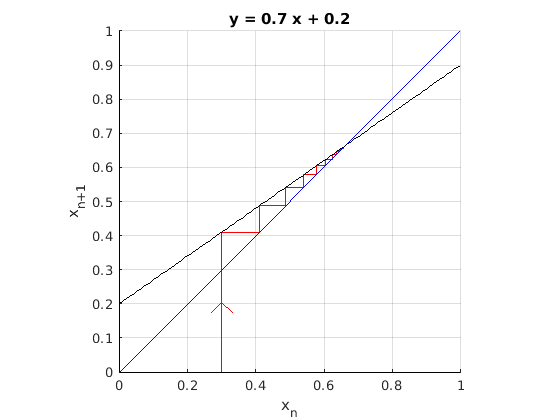
\includegraphics[width=7cm]{6_derivees_appl/affine1}\label{AFFINE1}}
\qquad
\subfloat[$x_{n+1}=2x_n-0.6$]{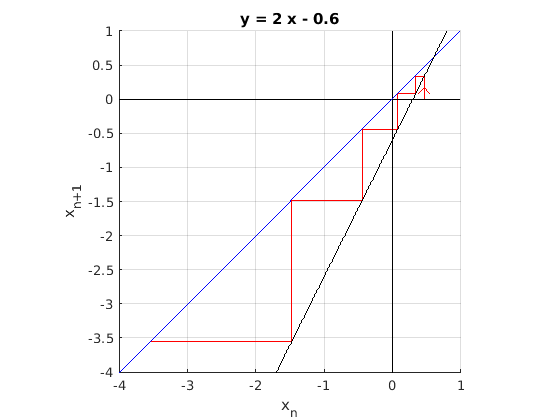
\includegraphics[width=7cm]{6_derivees_appl/affine2}\label{AFFINE2}}
\\
\subfloat[$x_{n+1} =-0.7x_n+0.68$]{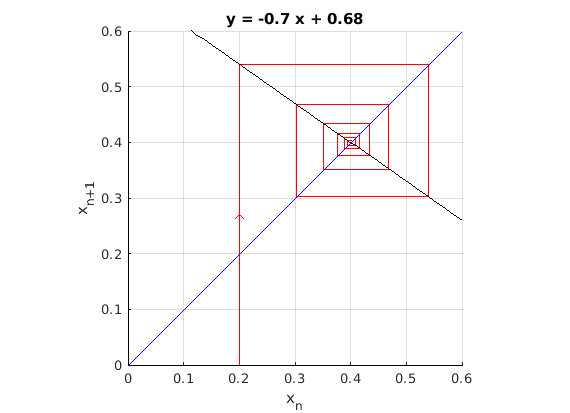
\includegraphics[width=7cm]{6_derivees_appl/affine3}\label{AFFINE3}} 
\qquad
\subfloat[$x_{n+1} = -2x_n+1.2$]{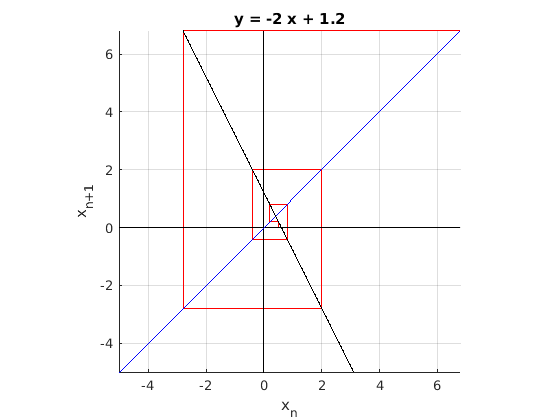
\includegraphics[width=7cm]{6_derivees_appl/affine4}\label{AFFINE4}}
\caption[Types de stabilité pour le point d'équilibre d'un
système dynamique discret de la forme $x_{n+1} = m x_n + b$]
{(a) Le point d'équilibre $p=2/3$ est asymptotiquement stable,  Le
  graphique contient l'orbite pour $x_0 = 0.3$.
(b) Le point d'équilibre $p=3/5$ est instable.  Le graphique contient
l'orbite pour $x_0 = 0.47$.
(c) Le point d'équilibre $p=2/5$ est asymptotiquement stable.  Le
graphique contient l'orbite pour $x_0 =0.2$.
(d) Le point d'équilibre $p=2/5$ est instable.  Le graphique contient
l'orbite pour $x_0 = 0.5$.}\label{AFFINE1-4}
\end{figure}

% \MATHfig{6_derivees_appl/affine1}{8cm}{Le point d'équilibre $p=2/3$ du
% système dynamique $x_{n+1} = 0.7x_n+0.2$}{Le point d'équilibre $p=2/3$
% du système dynamique $x_{n+1} = f(x_n)= 0.7x_n+0.2$ pour $n=0$, $1$,
% $2$, \ldots\ est asymptotiquement stable,  Le graphique contient
% l'orbite pour $x_0 = 0.3$.}{AFFINE1} 

% \MATHfig{6_derivees_appl/affine2}{8cm}{Le point d'équilibre $p=3/5$ du
% système dynamique $x_{n+1} = 2x_n-0.6$}{Le point d'équilibre $p=3/5$
% du système dynamique $x_{n+1} = f(x_n) = 2x_n -0.6 $ pour $n=0$, $1$,
% $2$, \ldots\ est instable.  Le graphique contient l'orbite pour
% $x_0 = 0.47$}{AFFINE2} 

% \MATHfig{6_derivees_appl/affine3}{8cm}{Le point d'équilibre $p=2/5$ du
% système dynamique $x_{n+1} =-0.7x_n+0.68$}{Le point d'équilibre
% $p=2/5$ du système dynamique $x_{n+1} = f(x_n)= -0.7x_n+0.68$ pour
% $n=0$, $1$, $2$, \ldots\ est asymptotiquement stable.  Le graphique
% contient l'orbite pour $x_0 = 0.2$}{AFFINE3}

% \MATHfig{6_derivees_appl/affine4}{8cm}{Le point d'équilibre $p=2/5$ du
% système dynamique $x_{n+1} = -2x_n+1.2$}{Le point d'équilibre $p=2/5$
% du système dynamique $x_{n+1} = f(x_n)=-2x_n +1.2$ pour $n=0$, $1$,
% $2$, \ldots\ est instable.  Le graphique contient l'orbite pour
% $x_0 = 0.5$}{AFFINE4}

Les exemples précédents justifient le résultat suivant.

\begin{focus}{\prp}
Nous considérons le système dynamique discret
\[
x_{n+1} = f(x_n) \quad \text{pour} \quad n=0, 1, 2, 3, \ldots
\]
où la fonction itérative est $y=f(x) = m x +b$.  Si $p$ est un point
d'équilibre de ce système dynamique discret alors ce point d'équilibre
est asymptotiquement stable si $|m|<1$ et instable si $|m|>1$.
\end{focus}

Comment pouvons-nous déterminer la stabilité asymptotique d'un point
d'équilibre $p$ d'un système dynamique discret
\[
x_{n+1} = f(x_n) \quad \text{pour} \quad n=0, 1, 2, 3, \ldots
\]
où $f$ n'est pas une fonction affine?

Supposons que $p$ soit un point d'équilibre pour un système dynamique
discret
\[
x_{n+1} = f(x_n) \quad \text{pour} \quad n =0, 1, 2 ,\ldots
\]
où $f$ est une fonction différentiable quelconque.  Nous savons que
$f(x) \approx g(x) = f(p) + f'(p) (x-p)$ pour $x$ très près de $p$.
Très près du point $p$, le système dynamique discret ci-dessus devrait
donc se comporter comme le système dynamique discret
\[
x_{n+1} = g(x_n) = f(p) + f'(p) (x_n-p) = m x_n + b \quad \text{pour} \quad
n=0,1,2,\ldots
\]
où $m = f'(p)$ et $b = f(p) - p\,f'(p)$.  En se basant sur le résultat
précédent pour les fonctions itératives de la forme $f(x) = mx+b$,
nous obtenons le résultat suivant.

\begin{focus}{\thm} \label{sdd_stab_th}
Soit $f:\RR \to \RR$ une fonction qui possède une dérivée continue.
Soit $p$ un point d'équilibre du système dynamique discret
\[
x_{n+1}=f(x_n) \quad \text{pour} \quad n=0, 1, 2, \ldots
\]
Le point d'équilibre $p$ est asymptotiquement stable si
$|f'(p)| < 1$.  Il est instable si $|f'(p)|>1$.  Nous ne pouvons rien
conclure lorsque $|f'(p)|=1$.
\end{focus}

La démonstration de ce résultat, que nous donnerons prochainement, est
une simple application des résultats du calcul différentiel que nous
avons présentés.

Revenons à notre équation logistique
\[
x_{n+1} = r x_n (1-x_n) \quad , \quad n=0,1,2,\ldots
\]
Les points d'équilibre sont les solutions de
\[
r x (1-x) = x \; .
\]
Si $x\neq 0$, nous pouvons diviser des deux cotés de l'égalité par $x$ pour
obtenir $r (1-x)=1$.  Ainsi, $x = 1 - 1/r$.  L'équation logistique a
donc deux points fixes: $x=0$ et $x=1-1/r$.

Si, comme à la section précédente, $x_n$ est la fraction de la
population maximale, le point fixe $x=0$ est simplement le fait que
s'il n'y a pas de bactéries initialement, il n'y en aura pas dans le
futur.   Dans le cas $r=1.1$, nous retrouvons l'état d'équilibre $x=1/11$
déjà observé.

Il n'est pas toujours possible de trouver algébriquement, comme nous
venons de le faire pour l'équation logistique, les points
d'équilibres.  Nous utilisons alors des méthodes numériques comme la
méthode de Newton pour estimer les points d'équilibre.

\begin{egg}
Nous avons vu que $p= 1/11$ est un point d'équilibre pour l'équation
logistique
\[
x_{n+1} = f(x_n) = r\, x_n (1-x_n) \quad \text{pour} \quad n=0, 1, 2, 3 \ldots
\]
où $r=1.1$.  Les orbites que nous avons calculées numériquement semblent
indiquer que ce point d'équilibre est asymptotiquement stable.

Posons $f(x) = r x (1-x)$.  Nous avons que $f'(x) = r(1-2x)$.  Ainsi, pour
$r=1.1$ et $x = p = 1/11$, nous obtenons
\[
f'(p) = 1.1 \left( 1 - 2\,\frac{1}{11}\right) = -0.9 \; .
\]
Puisque $|f'(p)|<1$, le point d'équilibre $p$ est asymptotiquement
stable.
\end{egg}

\begin{rmk}
Soit le système dynamique discret
\[
x_{n+1} = f(x_n) \quad , \quad n=0, 1, 2, \ldots
\]
Les points d'équilibre $p$ où $|f'(p)|=1$ sont en fait très
importants.  C'est une des conditions pour obtenir une
{\bfseries bifurcation}.  Si nous supposons que $f$ dépend d'un paramètre
$r$ (comme c'est le cas pour l'équation logistique) et que pour une
valeur $r_0$ de $r$ il existe un point d'équilibre $p$ tel que
$|f'(p)|=1$, alors le comportement du système dynamique discret pour
$r<r_0$ peut être très différant du comportement du système dynamique
discret pour $r>r_0$ si certaines conditions génériques sont
satisfaites.

Nous invitons le lecteur à tracer le graphe en forme de toile
d'araignée de l'équation logistique pour des valeurs de $r$ entre $2$
et $3$, et une condition initiale entre $0$ et $1$.  Puis, de répéter
cette même expérience avec des valeurs de $r$ entre $3$ et $3.447\ldots$
\ Qu'arrive-t-il lorsque $r$ devient plus grand que $3.447\ldots$?
Quand $r = 3.839\ldots$?

Lorsque $3<r<4$, le point $p=1-1/r$ est toujours un point
d'équilibre.  Par exemple, pour $r=13/4=3.25$, nous avons le point
d'équilibre $p=9/13=0.69230769231$.  Pourquoi les orbites ne
tendent-elles pas vers ce point d'équilibre?

Nous répondrons à certaines de ces questions à la prochaine section.

Le comportement des orbites de l'équation logistique lorsque $r$ varie
est fascinant.   Il existe un grand nombre de livres sur ce sujet.
\end{rmk}

\begin{proof}[\theory][Théorème~\ref{sdd_stab_th}]
La démonstration qu'un point fixe $p$ pour un système dynamique discret
\[
x_{n+1} = f(x_n) \quad , \quad n=0, 1, 2, 3, \ldots
\]
est asymptotiquement stable si $|f'(p)|<1$ et instable si $|f'(p)|>1$
repose sur le théorème de la moyenne.  Nous démontrons seulement que
$|f'(p)|<1$ implique la stabilité asymptotique du point d'équilibre
$p$ et laissons aux lecteurs le soin de démontrer que $|f'(p)|>1$
implique l'instabilité du point d'équilibre $p$.

Supposons que $f$ soit une fonction différentiable dont la dérivée
$f'$ est une fonction continue.  Puisque $|f'(p)|$ est strictement
plus petit que $1$ et $f'$ est continue, nous pouvons trouver une constante
$K$ plus grande ou égale à $|f'(p)|$ et plus petite que $1$, et une
petite valeur $\delta$ telle que $|f'(x)| \leq K<1$ pour tout $x$ dans
l'intervalle $I = ]p-\delta, p+\delta[$ qui contient $p$.

\subQ{i} Si $x_0 \in I$, alors $x_n \in I$ pour tout $n$.

En effet, supposons que $x_n$ soit dans $I$, alors $|x_n-p|<\delta$.  Grâce
au théorème de la moyenne, il existe $\zeta$ entre $p$ et $x_n$ tel que
$f(x_n) - f(p) = f'(\zeta)(x_n - p)$.  Notons que $\zeta \in I$ car $\zeta$
est entre $x_n$ et $p$.  Ainsi,
\[
|x_{n+1} - p| = |f(x_n) - f(p)| = |f'(\zeta)(x_n - p)|
\leq K | x_n - p | < |x_n - p| < \delta
\]
car $K<1$.  Il s'en suit que $x_{n+1}$ est aussi dans l'intervalle $I$.
Par induction, $x_n \in I$ pour tout $n$.

\subQ{ii} Encore grâce au théorème de la moyenne, ils existent $\zeta_n$
entre $x_n$ et $p$ tels que
$f(x_n) - f(p) = f'(\zeta_n)(x_n - p)$
avec $\zeta_n \in I$ car $\zeta_n$ est entre $x_n$ et $p$.  Nous avons donc
$|f'(\zeta_n)|\leq K$ pour tout $n$.  Ainsi,
\begin{align*}
|x_n -p| &= |f(x_{n-1}) - f(p)| = |f'(\zeta_{n-1})(x_{n-1} - p)|\\
&\leq K |x_{n-1} - p| = K |f(x_{n-2}) - f(p)|
= K |f'(\zeta_{n-2})(x_{n-2} - p)| \\
&\leq K^2 |x_{n-2} -p|\\
& \ldots\\
&\leq K^n |x_0 - p| \; .
\end{align*}

\subQ{iii} Nous avons donc que
\[
|x_n -p| \leq K^n |x_0-p|  \to 0 \quad \text{lorsque} \quad n \to \infty
\]
car
\[
\lim_{n\rightarrow \infty} K^n = 0
\]
pour $0<K<1$.

Toutes les orbites avec la condition initiale $x_0$ dans $I$
tendent donc vers $p$.
\end{proof}

\begin{egg}
Cet exemple provient de \cite{A}.

Le nombre de poissons d'une certaine espèce est gouverné par le
système dynamique discret
\begin{equation}\label{fish_harv}
p_{n+1} = r p_n (1-p_n) - h p_n  \quad \text{pour} \quad  0 < h < r
-1 < 2 
\end{equation}
où $p_n$ est le nombre de poissons au début de la $n^e$ saison de
pêche divisé par le nombre maximal de poissons que le milieu peut
supporter, $r$ est un facteur de croissance pour cette espèce de
poissons et $h$ est un facteur d'efficacité des pêcheurs. La valeur
$h$ est déterminée par le nombre de permis de pêche, l'équipement
utilisé par les pêcheurs, etc.  Le terme $-h\,p_n$ dans l'équation
(\ref{fish_harv}) représente la récolte à chaque année et a un effet
négatif sur la croissance de la population de poissons.

Lors d'une saison de pêche, si $h$ augmente, alors le nombre de
poissons capturés par les pêcheurs augmentera.  Si nous permettons une plus
grande valeur pour $h$ lors d'une saison de pêche, alors nous augmentons
l'effet négatif sur la croissance de la population.  Si $h$ est trop
grand, nous risquons de provoquer une diminution de la population de
poissons à long terme et de mettre ainsi en danger la survie de
cette espèce.  À long terme, il n'y aurait plus de poissons à capturer.

Le but est donc de choisir $h$ pour maximiser le nombre de poissons
capturés lors des futures saisons de pêche.  En d'autres mots, nous
voulons maximiser la récolte de poissons à long terme.  Cette récolte est
définie comme étant le produit du facteur d'efficacité $h$ des
pêcheurs avec l'état d'équilibre stable $p_h$ de la population de
poissons associé à cette valeur $h$.  En termes mathématiques, nous
voulons maximiser $R(h) = h\,p_h$.

La fonction itérative pour le système dynamique discret
(\ref{fish_harv}) est $f(p) = r p(1-p) - h p$.  Les points d'équilibre
du système dynamique discret (\ref{fish_harv}) sont donnés par les
solutions de $p = f(p)$.  Nous trouvons $p_0 = 0$ et $p_h = (r-h-1)/r$.  Le
point d'équilibre $p_h$ est positif car nous assumons $h < r-1$.

Nous utilisons le théorème~\ref{sdd_stab_th} pour déterminer si le point
d'équilibre $p_h$ est stable.  Puisque $f'(p) = r - h - 2r p$, nous
obtenons $|f'(p_h)| = |2 + h - r|$.  Pour que le point d'équilibre $p_h$
soit stable, nous devons donc exiger que
\[
|f'(p_h)| = |2 + h - r|<1 \Leftrightarrow -1 < 2 + h - r < 1
\Leftrightarrow -3 + r < h < r - 1 \ .
\]
C'est effectivement le cas pour $0 \leq h < r -1 < 2$.  Notez que
$|f'(p_0)| = |r - h| > 1$ pour $h < r -1$ et donc le point d'équilibre
$p_0$ est instable.

Considérons la récolte à long terme $R(h) = h\,p_h = h(r-h-1)/r$.
Nous avons $R'(h) = (r-2h-1)/r$ et le seul point critique est
$h = H \equiv (r-1)/2$.  Nous résumons dans le tableau suivant
l'information que nous avons au sujet de la fonction $R$.
\[
\begin{array}{c|c|c|c|c|c}
h & 0 & 0 < h < H & H & H < h < r-1 & r-1 \\
\hline
R(h) & 0 & + & \rule{0em}{1em} (r-1)^2/(4r) & + & 0 \\
\hline
R'(h) & + & + & 0 & - & - \\
\hline
 & & & \text{max. local} & & \\
\end{array}
\]
La récolte $R(h)$ est donc maximale pour $h = H$.  L'état d'équilibre
de la population de poissons pour $h = H$ est alors
$p_H = (r-1)/(2r)$.  Comme nous avons démontré, le point d'équilibre 
$p_H$ est stable et donc $\displaystyle \{p_n\}_{n=1}^\infty$ converge vers
ce point d'équilibre.  La récolte maximale de poissons à long terme
sera $R(H) = H\,p_H = (r-1)^2/(4r)$.
\label{discrete_fish_probl}
\end{egg}

\subsection{Étude des orbites périodiques \theory}

\begin{egg}
Pour l'équation logistique
\[
x_{n+1} = f(x_n) = r\, x_n(1-x_i) \quad \text{pour} \quad n=0, 1, 2, 3, \ldots
\]
avec $r=3.2$, quelle que soit la condition initiale $x_0$ entre $0$ et
$1$ que nous choisissons, l'orbite
$\displaystyle \left\{ x_n\right\}_{n=0}^\infty$ ne tend pas vers un
point d'équilibre comme nous pouvons constater avec les données dans la
colonne de gauche du tableau~\ref{HS_LOGISTIC4}.  Remarquons que
\[
x_n =
\begin{cases}
0.5130445095\ldots &\quad \text{si $n$ est pair} \\
0.7994554905\ldots &\quad \text{si $n$ est impair}
\end{cases}
\]
pour $n$ assez grand.  L'orbite oscille entre ces deux valeurs.
\label{eggper1}
\end{egg}

\begin{egg}
Comme à l'exemple précédent, pour l'équation logistique
\[
x_{n+1} = f(x_n) = r\, x_n(1-x_n) \quad , \quad n =0, 1, 2, 3, \ldots
\]
avec $r=3.47$, l'orbite $\displaystyle \left\{ x_n\right\}_{n=0}^\infty$
ne tend pas vers un point d'équilibre quelle que soit la condition
initiale $x_0$ entre $0$ et $1$ que nous choisissons.  Cependant, à partir
des données dans la colonne de droite du Tableau~\ref{HS_LOGISTIC4},
nous pouvons conclure que
\[
x_n =
\begin{cases}
0.40291365318\ldots &\quad \text{si} \quad n=4k \\
0.83479261718\ldots &\quad \text{si} \quad n=4k+1 \\
0.47856124509\ldots &\quad \text{si} \quad n=4k+2 \\
0.86590511786\ldots &\quad \text{si} \quad n=4k+3
\end{cases}
\]
pour $k$ assez grand.  L'orbite est la répétition de ces quatre
valeurs, toujours dans le même ordre.
\label{eggper2}
\end{egg}

\begin{table}
{\scriptsize
\begin{center}
\begin{tabular}{c|c}
\cline{1-2}
  $n$   &  $x_n$  \\ 
\cline{1-2}
$0$ & $0.40000000000\ldots$ \\ 
$\vdots$ & $\vdots$ \\
$50001$ & $0.79945549047\ldots$ \\ 
$50002$ & $0.51304450953\ldots$ \\ 
$50003$ & $0.79945549047\ldots$ \\ 
$50004$ & $0.51304450953\ldots$ \\ 
$50005$ & $0.79945549047\ldots$ \\ 
$50006$ & $0.51304450953\ldots$ \\ 
$50007$ & $0.79945549047\ldots$ \\ 
$50008$ & $0.51304450953\ldots$ \\ 
$50009$ & $0.79945549047\ldots$ \\ 
$50010$ & $0.51304450953\ldots$ \\ 
\cline{1-2}
\end{tabular}
\qquad\qquad
\begin{tabular}{c|c}
\cline{1-2}
  $n$   &  $x_n$  \\ 
\cline{1-2}
$0$ & $0.40000000000\ldots$ \\ 
$\vdots$ & $\vdots$ \\
$50001$ & $0.83479261718\ldots$ \\ 
$50002$ & $0.47856124509\ldots$ \\ 
$50003$ & $0.86590511786\ldots$ \\ 
$50004$ & $0.40291365318\ldots$ \\ 
$50005$ & $0.83479261718\ldots$ \\ 
$50006$ & $0.47856124509\ldots$ \\ 
$50007$ & $0.86590511786\ldots$ \\ 
$50008$ & $0.40291365318\ldots$ \\ 
$50009$ & $0.83479261718\ldots$ \\
$50010$ & $0.47856124509\ldots$ \\ 
\cline{1-2}
\end{tabular}
\end{center}
}
\caption[Orbites de l'équation logistique $x_{n+1}=r x_n ( 1-x_n)$
pour $r=3.2$ et $r=3.47\ldots$]{Deux orbites de l'équation logistique
avec la condition initiale $x_0 = 0.4$.  $r=3.2$ pour le tableau à
gauche et $r=3.47\ldots$ pour le tableau de droite. \label{HS_LOGISTIC4}}
\end{table}

Les deux exemples précédents justifient la définition suivante.

\begin{focus}{\dfn}
Soit $f:X \to X$ avec $X \subset \RR$.  Si
$\displaystyle \left\{ x_n \right\}_{n=0}^\infty$ est une orbite du
système dynamique discret
\[
x_{n+1} = f(x_n) \quad , \quad n=0, 1, 2, \ldots
\]
pour laquelle il existe un entier positif $k$ tel que $x_n = x_{n+k}$
pour $n=0$, $1$, $2$, \ldots, alors l'orbite 
$\displaystyle \left\{ x_n \right\}_{n=0}^\infty$ est appelée une
{\bfseries orbite périodique}\index{Système dynamique discret!orbite
  périodique}
ou {\bfseries solution périodique}\index{Système dynamique
  discret!solution périodique}.  Les
points de cette orbite sont appelés des
{\bfseries points périodiques}\index{Système dynamique discret!point
  périodique} pour $f$.

Si $k$ est le plus petit entier positif tel que $x_n = x_{n+k}$, alors
$k$ est la {\bfseries période}\index{Système dynamique discret!période
  d'une orbite} de l'orbite.
\end{focus}

\begin{egg}
À l'exemple~\ref{eggper1}, $p=0.5130445095\ldots$ est un point
périodique et l'orbite avec la condition initiale $x_0=p$ est une
orbite périodique de période $2$ (figure~\ref{HS_LOGISTIC5}).

À l'exemple~\ref{eggper2}, $p=0.40291365318\ldots$ est un point
périodique et l'orbite avec la condition initiale $x_0=p$ est une
orbite périodique de période $4$ (figure~\ref{HS_LOGISTIC6}).
\end{egg}

\begin{figure}
\centering
\subfloat[$r=3.2$]{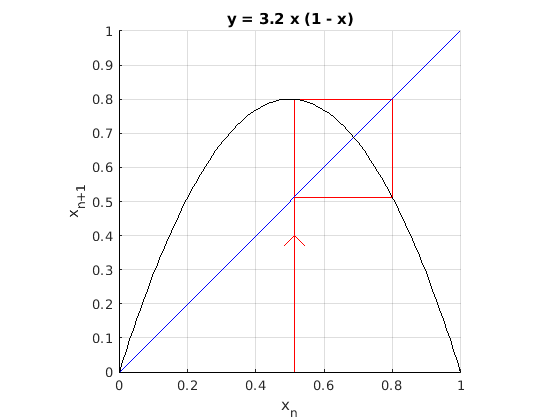
\includegraphics[width=7cm]{6_derivees_appl/hs_logistic5}\label{HS_LOGISTIC5}}
\qquad
\subfloat[$r=3.47$]{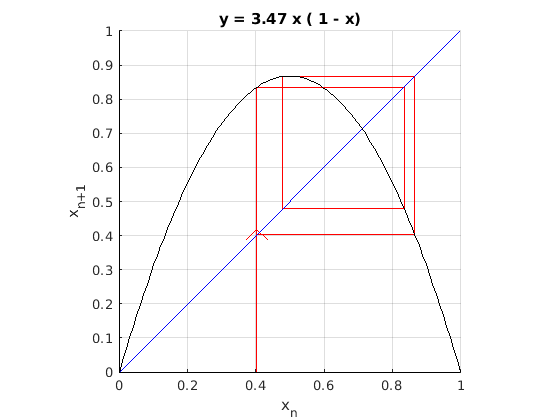
\includegraphics[width=7cm]{6_derivees_appl/hs_logistic6}\label{HS_LOGISTIC6}}
\caption[Orbites périodiques de période $2$ et $4$ pour l'équation logistique]
{(a) Orbite périodique de période $2$ pour l'équation logistique avec
$r=3.2$.  (b) Orbite périodique de période $4$ pour l'équation
logistique avec $r=3.47$.}\label{HS_LOGISTIC56}
\end{figure}

% \MATHfig{6_derivees_appl/hs_logistic5}{8cm}{Orbite périodique de période
% $2$ pour l'équation logistique avec $r=3.2$}{Orbite périodique de
% période $2$ pour l'équation logistique avec $r=3.2$}{HS_LOGISTIC5}

% \MATHfig{6_derivees_appl/hs_logistic6}{8cm}{Orbite périodique de période
% $4$ pour l'équation logistique avec $r=3.47$}{Orbite périodique de
% période $4$ pour l'équation logistique avec $r=3.47$}{HS_LOGISTIC6}

Dans les deux exemples précédents, quelle que soit la condition
initiale $x_0$, l'orbite
$\displaystyle \left\{ x_n\right\}_{n=0}^\infty$ se comporte de plus
en plus comme l'orbite périodique (figure~\ref{HS_LOGISTIC7}).  Nous
avons donc une notion de stabilité asymptotique pour les solutions
périodiques.

\MATHfig{6_derivees_appl/hs_logistic7}{8cm}{Stabilité de l'orbite de
période $4$ pour l'équation logistique avec $r=3.47$}{Une orbite qui
\lgm converge\rgm\ vers l'orbite périodique de période $4$ pour
l'équation logistique avec $r=3.47$.  La condition initiale est
$x_0=0.1$}{HS_LOGISTIC7}

\begin{focus}{\dfn}
\index{Système dynamique discret!solution périodique!asymptotique stabilité}
Soit $f: X \to X$ avec $X \subset \RR$, et
$\displaystyle \left\{ x_n \right\}_{n=0}^\infty$ une orbite périodique
de période $k$ pour le système dynamique discret
\[
x_{n+1} = f(x_n) \quad , \quad n=0, 1, 2, 3, \ldots
\]
Cette orbite est {\bfseries asymptotiquement stable} si $p$, un point
quelconque de l'orbite, est un point fixe asymptotiquement stable pour
la fonction
\[
 g = \underbrace{f\circ f \circ \ldots \circ f}_{\text{$k$ copies de $f$}} \; .
\]
\end{focus}

\begin{rmk}
Nous invitons le lecteur à démontrer que la définition précédente est
indépendante du choix du point périodique $p$ de l'orbite.
\end{rmk}

Le lecteur peut utiliser l'application qui se trouve sur le site\\
\href{https://mysite.science.uottawa.ca/bdionne/math_stat/fractal/fractal3_en.html}{https://mysite.science.uottawa.ca/bdionne/math\_stat/fractal/fractal3\_en.html} pour explorer le comportement des
orbites de l'équation logistique de la définition \ref{defOfLogEqu}
lorsque $r$ varie.

}  % End of theory

\section{Exercices}

\subsection{Dérivées d'ordres supérieures}

\begin{question}
Calculez la dérivée première et seconde des fonctions suivantes.
\begin{center}
\begin{tabular}{*{2}{l@{\hspace{0.5em}}l@{\hspace{3em}}}l@{\hspace{0.5em}}l}
\subQ{a} & $\displaystyle h(y) = y^{10}-y^9$ &
\subQ{b} & $\displaystyle f(x) = \frac{3+x}{2x}$ &
\subQ{c} & $\displaystyle f(x) = x^2 e^x$ \\
\subQ{d} & $\displaystyle f(x) = \frac{1+x}{e^x}$ &
\subQ{e} & $\displaystyle g(z) = (z+4)\ln(z)$ &
\subQ{f} & $\displaystyle F(w) = e^w \ln(w)$ \\
\subQ{g} & $\displaystyle f(x) = \ln(x^7)$ &
\subQ{h} & $\displaystyle f(z) = \frac{1+e^{-z}}{1+e^z}$ &
\subQ{i} & $\displaystyle F(y) = \frac{\ln(y)}{e^y}$ \\[0.9em]
\subQ{j} & $\displaystyle f(x) = 1 + x^{4/5}$ &
\subQ{k} & $\displaystyle f(x)= \frac{2+x^3}{1+x^2}$
\end{tabular}
\end{center}
\label{6Q1}
\end{question}

\begin{question}[\life \eng]
Si $H(\theta) = \theta \sin(\theta)$, évaluez $H'(\theta)$ et $H''(\theta)$.
\label{6Q2}
\end{question}

\begin{question}
Nous laissons tomber un objet d'une hauteur de $100$ m sur Jupiter.  Nous
assumons qu'il n'y a pas de friction sur l'objet.  L'accélération dû à
la gravité de Jupiter est $g = 22.88$ m/s$^2$.  Combien de temps
s'écoule-t-il avant que l'objet frappe le sol?  À quel vitesse l'objet
frappe-t-il le sol? 
\label{6Q3}
\end{question}

\begin{question}
Sur Jupiter, nous lançons un objet vers le haut à une vitesse de $10$ m/s
à partir d'une hauteur de $100$ m.  Nous assumons qu'il n'y a pas de
friction sur l'objet.  L'accélération dû à la gravité de Jupiter est
$g = 22.88$ m/s$^2$. Combien de temps s'écoule-t-il avant que l'objet
atteigne sa plus grande distance du sol?  Quelle est la hauteur de
l'objet à ce moment?  Combien de temps s'écoule-t-il avant que l'objet
frappe le sol?  À quel vitesse l'objet frappe-t-il le sol?
\label{6Q4}
\end{question}

\subsection{Graphes de fonctions}

\begin{question}
Le graphe d'une fonction $f$ est donné ci-dessous.
\PDFgraph{6_derivees_appl/graph_funct1}

\subQ{a} Donnez les point critiques.\\
\subQ{b} Donnez les valeurs de $x$ où $f'(x)>0$.\\
\subQ{c} Donnez les valeurs de $x$ où $f'(x)<0$.\\
\subQ{d} Donnez les valeurs de $x$ où $f''(x)>0$.\\
\subQ{e} Donnez les valeurs de $x$ où $f''(x)<0$.
\label{6Q5}
\end{question}

\begin{question}
Dessinez le graphe d'une fonction qui possède les propriétés suivantes:

\subQ{a} Une fonction positive qui possède une dérivée strictement
croissante.\\
\subQ{b} Une fonction avec une dérivée négative et strictement croissante.
\label{6Q6}
\end{question}

\begin{question}
Le graphe suivant représente la position $x$ d'une voiture dans les montagnes
russes (i.e. \lgm roller coaster\rgm) en fonction du temps.  À quelles
moments la voiture se déplace-t-elle le plus rapidement?  À quelles moments
la voiture accélère-t-elle le plus rapidement?  À quelles moments la voiture
décélère-t-elle le plus rapidement?  Expliquez votre réponse.
\PDFgraph{6_derivees_appl/graph_funct4}
\label{6Q7}
\end{question}

\begin{question}
La position vertical d'un objet à partir du sol est décrite par la
fonction $p(t) = -5.2 t^2 - 2 t + 50$.  Supposons que la direction
positive soit vers le haut.  Cette équation n'est pas valide sur la
terre mais sur une planète plus lourde que la terre.  La position est
donnée en mètres et le temps en secondes.

\subQ{a} Trouvez la vélocité et l'accélération de l'objet en fonction
du temps.\\
\subQ{b} Tracez le graphe de la position en fonction du temps à l'aide
des résultats en (a).\\
\subQ{c} Si l'objet part du haut d'une tour, quelle est la hauteur de
la tour?  Dans quelle direction et à quelle vitesse avons-nous lancé (si
nous avons lancé) l'objet, vers le haut ou vers le bas?  Quelle est
l'accélération dû à la gravité sur cette planète?
\label{6Q8}
\end{question}

\begin{question}
Dans son nouveau programme d'exploration des objets célestes, la NASA
utilise des sondes spatiales inhabitées.  Une expérience conduite par
une sonde se trouvant à $100$ m au dessus de la lune Deimos de mars
consistait à lancer vers le haut un objet à une vitesse de $5$ m/s
pour analyser sa trajectoire. L'accélération dû à la gravité est de
$2.15\times 10^{-3}$ m/s$^2$ sur cette lune.

\subQ{a} Trouvez la vélocité et la position de l'objet en fonction du
temps.\\
\subQ{b} Quelle est la hauteur maximale atteinte par l'objet?\\
\subQ{c} Combien de temps faut-il à l'objet pour revenir à la hauteur
de départ?  Quelle est la vélocité de l'objet à ce moment?\\
\subQ{d} Combien de temps faut-il à l'objet pour atteindre le sol de
la lune? Quelle est la vélocité de l'objet à ce moment?\\
\subQ{e} Tracez le graphe de la vélocité et de la position de l'objet
en fonction du temps.
\label{6Q9}
\end{question}

\begin{question}
Le graphe de $g'$ est donné ci-dessous.
\PDFgraph{6_derivees_appl/derivative2}
Si $g(0)= 2$, tracez un graphe possible pour $g$.  Soyez aussi précis que
possible.
\label{6Q10}
\end{question}

\begin{question}
Utilisez le graphe du taux de variation instantanée de la fonction $w$
qui est donné ci-dessous pour tracer le graphe de la fonction $w$ si $w(0)=1$.
\PDFgraph{6_derivees_appl/derivative3}
\label{6Q11}
\end{question}

\begin{question}[\life]
Le volume de déchets au temps $t$ produit par deux villes est donnée
par $\displaystyle V_a(t) = t^2 - 3t + 16$ pour la ville $A$ et
$V_b(t) = 20 + 3t$ pour la ville $B$.  Le volume est mesuré en m$^3$
et le temps $t$ est mesuré en années.  Si les déchets contiennent
$\rho(t) = 1.2 - 0.1 t$ g/m$^3$ d'un certain produit toxique au temps
$t$, répondre aux questions suivantes.

\subQ{a} Exprimez la masse du produit toxique en fonction du temps.\\
\subQ{b} Exprimez le taux de variation de la masse en fonction du temps.\\
\subQ{c} À l'aide du taux de variation calculé en (b), tracez le
graphe de la masse en fonction du temps pour $t\geq 0$.  Est-ce que
les efforts des deux villes d'éliminer le produit toxique de leurs
déchets sont encourageants au départ?
\label{6Q12}
\end{question}

\begin{question}[\life]
La masse d'une culture en fonction du temps est donnée par
$M(t) = 1 + t^2$ et le volume en fonction du temps est donné par
$V(t) = 1+t$.  La masse est mesurée en grammes, le volume en cm$^3$ et le
temps en jours.

\subQ{a} Exprimez la densité en fonction du temps.\\
\subQ{b} Calculez la dérivée de la densité.\\
\subQ{c} Pour quelles valeurs de $t$ a-t-on que la densité est
strictement croissante?\\
\subQ{d} À l'aide de la dérivée calculée en (b), tracez le graphe de
la densité en fonction du temps.
\label{6Q13}
\end{question}

\begin{question}[\life]
En l'absence d'influences externes, la croissance annuelle d'une
population dépend seulement de la production annuelle moyenne par
individu.  Supposons que la production annuelle moyenne par individu
lorsqu'il y a $p$ individus soit donnée par
$\displaystyle f(p) = 2\left( 1- \frac{p}{1000}\right)$.

\subQ{a} Exprimez la taille $T$ de la population (i.e. nombre d'individus)
après un an en fonction de la taille de la population au début de l'année.\\
\subQ{b} Calculez la dérivée de $T$ par rapport à la population
initiale $p$.\\
\subQ{c} À l'aide de la dérivée calculée en (b), tracez le graphe de
$T$ pour $0 < p < 1000$.
\label{6Q14}
\end{question}

\begin{question}
Soit $f$ une fonction continue qui satisfait:\\
\subQ{a} $f\,'(x)>0$ si $-2<x<1$,\\
\subQ{b} $f\,'(x)=0$ si $x=-2$ ou $x=1$,\\
\subQ{c} $f\,'(x)<0$ si $x>1$ ou $x<-2$, et\\
\subQ{d} $f(x)>0$ pour tout $x$.\\
Tracez (de façon approximative) le graphe de cette fonction.
Expliquez en une phrase le sens graphique des énoncés.
\label{6Q15}
\end{question}

\begin{question}
Trouvez les points où la fonction
$\displaystyle f(x)=\frac{e^{2x^2}}{x}$ possède un 
minimum ou un maximum local.
\label{6Q16}
\end{question}

\begin{question}
Soit $\displaystyle f(x) = x\sqrt{5-x}$ pour $x<5$.  Répondre aux questions
suivantes.

\subQ{a} Trouvez les intervalles où la fonction $f$ est strictement
croissante et décroissante.\\
\subQ{b} Trouvez les points où la fonction $f$ a des maximums et
minimums locaux et calculez la valeur de ces maximums et minimums
locaux.\\
\subQ{c} Trouvez les intervalles de concavité et les points
d'inflexion.\\
\subQ{d} Utilisez l'information obtenue précédemment pour tracer le
graphe de $f$.
\label{6Q17}
\end{question}

\begin{question}[\life \eng]
Soit $\displaystyle f(x) = x - 2\sin(x)$ pour $0<x<3\pi$. Répondre aux
questions suivantes.

\subQ{a} Trouvez les intervalles où la fonction $f$ est strictement
croissante et décroissante.\\
\subQ{b} Trouvez les points où la fonction $f$ a des maximums et
minimums locaux et calculez la valeur de ces maximums et minimums
locaux.\\
\subQ{c} Trouvez les intervalles de concavité et les points
d'inflexion.\\
\subQ{d} Utilisez l'information obtenue précédemment pour tracer le
graphe de $f$.
\label{6Q18}
\end{question}

\begin{question}
Tracez un graphe de $y = f(x)$ en utilisant les données suivantes.
\[
\begin{array}{c|c|c|c|c|c|c|c|c|c}
x & x<x_1 & x_1 & x_1<x<x_2 & x_2 & x_2<x<x_3 & x_3 & x_3<x<x_4 &
x_4 & x>x_4 \\
\hline
f'(x) & - & - & - & 0 & + & + & + & 0 & - \\
f''(x) & - & 0 & + & + & + & 0 & - & - & -
\end{array}
\]
\label{6Q19}
\end{question}

\begin{question}[4 points]
Nous considérons la fonction $f$ qui possède les propriétés suivantes:
{\renewcommand{\labelitemi}{\textbullet}
\begin{itemize}
\item $f$ est une fonction continue sur son domaine;
\item $\displaystyle \lim_{x\to -\infty}f(x)=2$,
$\displaystyle \lim_{x\to 1}f(x)=-2$,
$\displaystyle \lim_{x\to 3^-} f(x) = -\infty$ et
$\displaystyle \lim_{x\to 3^+}f(x)= \infty$;
\item $f(x)$ n'est pas définie en $x=3$;
\item $f'(x)$ n'est pas définie en $x=1$;
\item $f'(x)<0$ pour $x<1$, $2 < x < 3$ et $3 < x < 4$;
\item $f'(x)>0$ pour $1 < x < 2$ et $x > 4$;
\item $f''(x)<0$ pour $x<3$, $x\neq 1$;
\item $f''(x)>0$ pour $x>3$.
\end{itemize}
}
\subQ{a} Donnez le domaine de $f$.\\
\subQ{b} Déterminez les intervalles où $f$ est croissante et où $f$
est décroissante.\\
\subQ{c} Déterminez les intervalles où $f$ est convexe et
où $f$ est concave.\\
\subQ{d} Tracez le graphe de $f$ en prenant soin d'indiquer les points
critiques, asymptotes, point d'inflexions, \ldots
\label{6Q20}
\end{question}

\begin{question}
Pour chacune des fonctions ci-dessous, utilisez l'information fourni
par la dérivée première et seconde pour tracer son graphe.  Bien
indiquer où la fonction est strictement croissante et décroissante, où
la fonction est concave et convexe, les maximums et minimums locaux,
les points d'inflexions, les asymptotes horizontales et verticales,
etc.
\begin{center}
\begin{tabular}{*{1}{l@{\hspace{0.5em}}l@{\hspace{6em}}}l@{\hspace{0.5em}}l}
\subQ{a} & $h(x) = x^3 - 3x + 3$ &
\subQ{b} & $h(x) = x^3 - 6x^2 - 15 x + 3$ \\
\subQ{c} & $f(x) = x + 4/x^2$ &
\subQ{d} & $\displaystyle f(x) = (1-x)e^x$ \\
\subQ{e} & $\displaystyle g(z) = \frac{e^z}{z^2}$ &
\subQ{f} & $F(z) = z^3/e^z$ \\[0.5em]
\subQ{g} & $T(t) = (1-t^2) e^t$\ ,\ $-1 \leq t \leq 1$ &
\subQ{h} & $G(x) = \sqrt{x}\; e^{-x}$\ ,\ $x\geq 0$ \\
\subQ{i} & $\displaystyle f(x) = \frac{x^3}{1+x^3}$  &
\subQ{j} & $\displaystyle f(x) = \frac{2}{x^2} - \frac{3}{x^3}$ \\[0.8em]
\subQ{k} & $\displaystyle f(x) = (x+4)e^{-x}$ &
\subQ{l} & $\displaystyle f(x) = \frac{2}{x} -\frac{6}{x^3}$ \\[0.5em]
\subQ{m} & $\displaystyle f(x) = \frac{e^x}{x-1}$ &
\subQ{n} & $\displaystyle f(x) = \frac{x}{x^3+1}$ \\[0.5em]
\subQ{o} & $\displaystyle f(x) = x \ln(x)$ & &
\end{tabular}
\end{center}
\label{6Q21}
\end{question}

\begin{question}[\life \eng]
Pour chacune des fonctions ci-dessous, utilisez l'information fourni
par la dérivée première et seconde pour tracer son graphe.  Bien
indiquer où la fonction est strictement croissante et décroissante, où
la fonction est concave et convexe, les maximums et minimums locaux,
les points d'inflexions, les asymptotes horizontales et verticales,
etc.
\begin{center}
\begin{tabular}{*{1}{l@{\hspace{0.5em}}l@{\hspace{6em}}}l@{\hspace{0.5em}}l}
\subQ{a} & $\displaystyle y = \sin^2(x) -2 \cos(x)$ &
\subQ{b} & $f(\theta) = \theta + 3 \cos(\theta) \ , \ 0\leq \theta \leq 4\pi$
  \\
\subQ{c} & $h(t) = e^{-t} \sin(t) \ , \ 0\leq \theta \leq 4\pi$ & &
\end{tabular}
\end{center}
\label{6Q22}
\end{question}

\subsection{Optimisation}

\begin{question}[\life]
Le nombre de bactéries dans un milieu riche en substances nutritives est
décrit par
\[
N(t) = 5000 + \frac{30000\,t}{100+t^2}
\]
où $t$ est le temps.  Trouvez le nombre maximal de bactéries que nous
pourrons observer (i.e.  trouvez le maximum absolu pour $t\geq 0$). 
\label{6Q23}
\end{question}

\begin{question}[\life]
Nous considérons une espèce d'oiseaux dont le rapport $P$ du nombre moyen
de poussins qui survivent en fonction du nombre $x$ d'oeufs pondus est
donné par la fonction $P(x) = 1/(1+0.5 x^2)$.   Le nombre total de
poussins qui survivent en fonction du nombre d'oeufs pondus est donc
donné par $S(x) = x\,P(x)$. Trouvez le nombre de poussins qui 
survivent si un oiseau de cette espèce pond $5$, $10$ et $20$ oeufs.
Tracez le graphe de $S$.  Quelle est la meilleure stratégie pour cette
espèce d'oiseaux?  C'est-à-dire, combien d'oeufs devrait pondre un
oiseau de cette espèce pour avoir le plus grand nombre possible de
poussins qui survivent.

Dans ce problème, il faut comprendre que les valeurs de $S$ sont des
moyennes pour l'espèce d'oiseaux.  C'est pour cela que $S$ peut être
un nombre réel; $S$ n'est pas obligé d'être un entier.  Un oiseau ne
peut pas avoir $2.5$ poussins mais une population peut avoir en
moyenne $2.5$ poussins par individu.
\label{6Q24}
\end{question}

\begin{question}[\eco]
À un prix de \$50.00 l'unité, un jardinier peut vendre $100$
pommiers.  S'il augmente le prix par unité de \$1.00, il va vendre
$4$ pommiers de moins.  De même, s'il baisse le prix de
\$1.00, il va vendre $4$ pommiers de plus.  Le coût de production
d'un pommier est de \$9.00.  Calculer le prix par pommier qui maximise
le profit du jardinier.  {\bfseries Ne pas oublier} d'expliquer
pourquoi votre r\'eponse donne un maximum absolu.
\label{6Q25}
\end{question}

\begin{question}
Les questions suivantes font référence à une fonction continue
$f: [a,b] \rightarrow \RR$.

\subQ{a} Tracez un graphe pour $f$ si $f$ a un maximum absolu et un
minimum absolu entre $a$ et $b$.\\
\subQ{b} Tracez un graphe pour $f$ si $f$ est une fonction différentiable qui
a un maximum absolu à $x=a$, un minimum absolu à $x=b$ et aucun point
critique.  Décrire en une phrase cette fonction.\\
\subQ{c} Tracez un graphe pour $f$ si $f$ a un maximum absolu et un
minimum absolu entre $a$ et $b$, et $f'(x)\neq 0$ pour tout $x \in [a,b]$ où
la dérivée existe.
\label{6Q26}
\end{question}

\begin{question}
Pour chacune des fonctions ci-dessous, trouvez le maximum absolu et le
minimum absolu sur l'intervalle donné.
\begin{center}
\begin{tabular}{*{1}{l@{\hspace{0.5em}}l@{\hspace{3em}}}l@{\hspace{0.5em}}l}
\subQ{a} & $f(x) = 2 + x e^{-x} \ , \ 0.5 \leq x \leq 2$ &
\subQ{b} & $f(x) = x^3 - 3x \ , \ -2\leq c \leq 2$ \\[0.7em]
\subQ{c} & $\displaystyle f(x) = \frac{x}{x^2+x+1} \ , \ -2 \leq x \leq 0$ &
\subQ{d} & $f(x) = 5x(1-x)(2-x) - 1 \ , \ 0 \leq x \leq 1$ \\[0.7em]
\subQ{e} & $f(x)=x^{1/2}(x-4)^2 \ , \ 0.5 \leq x \leq 6$ & &
\end{tabular}
\end{center}
\label{6Q27}
\end{question}

\begin{question}
Trouvez le maximum absolu et le minimum absolu de $F(x) = |1-x|$ pour
$-2\leq x \leq 3$.
\label{6Q28}
\end{question}

\begin{question}
Tracez le graphe de $g(y) = y/(1+y^2)$ pour $0\leq y \leq 2$ a l'aide
de la dérivée premières et de la dérivée deuxième de $g$.

\subQ{a} Donnez les points où il y a un maximum ou minimum local.\\
\subQ{b} Donnez les points où il y a un maximum absolu et donnez
ce maximum.\\
\subQ{c} De même, donnez les points où il y a un minimum absolu et
donnez ce minimum.
\label{6Q29}
\end{question}

\begin{question}
Trouvez le point de la droite $y=4x+7$ qui est le plus près de l'origine.
\label{6Q30}
\end{question}

\begin{question}
L'aire d'un rectangle dont les côtés sont de longueurs $x$ et $y$
est $A = x y$.  Le périmètre de ce rectangle est $P = 2x + 2y$.

\subQ{a} Minimisez $P$ si $A$ est fixe.\\
\subQ{b} Maximisez $A$ si $P$ est fixe.
\label{6Q31}
\end{question}

\begin{question}
Nous voulons construire un enclos pour faire l'élevage de faisans.
l'enclos doit être rectangulaire et doit être partagé en trois
sections de même aire comme dans l'illustration ci-dessous.  Si nous avons
$3\,600$ m de clôture pour construire l'enclos.  Quelles sont les
dimensions du plus grand enclos que nous puissions construire?  Quelle est
alors l'aire de chacune des sections?

\PDFgraph{6_derivees_appl/fence}
\label{6Q32}
\end{question}

\begin{question}
Trouvez les dimensions $x$ et $y$ de la section transversale d'une
poutre de bois découpée d'un tronc d'arbre (circulaire) de $30$ cm de
rayon pour que la section transversale soit d'aire maximale.\\
Suggestion: cela revient à trouver le rectangle d'aire maximale qui
peut être inscrit dans un cercle ayant un diamètre de $30$ cm.
\label{6Q33}
\end{question}

\begin{question}
Vous campez à trois mètres de la rive d'une rivière.  Vous remarquez
qu'une tente à quatre mètres de la rive vient de
prendre feu.  Immédiatement, vous prenez une chaudière à l'intérieur
de votre tente (vous êtes une personne prévoyant qui amène toujours
une chaudière en camping), courez à la rivière pour remplir votre
chaudière, et allez à la tente pour éteindre le feu.  Quelle position
$x$ le long de la rivière minimisera la distance à parcourir (et donc
minimisera le temps d'intervention)?
\PDFgraph{6_derivees_appl/feu}
\label{6Q34}
\end{question}

\begin{question}
Une clôture de 2 m de haut longe un immeuble à 1 m de celui-ci sur
toute sa longueur.  Quelle est la longueur minimal de l'échelle qui
passe par dessus la clôture et s'appuie contre le mur de
cet immeuble?
\label{6Q35}
\end{question}

\begin{question}[\life]
Pour augmenter leur chance de survie, les animaux tentent de maximiser
le rapport entre la quantité de nourriture qu'ils récoltent et le
risque pour acquérir cette nourriture.  Par exemple, les fleurs qui
produisent une grande quantité de nectar permettent aux abeilles de
récolter une grande quantité de nectar mais ces fleurs attirent aussi
d'autres animaux qui sont des prédateurs pour les abeilles.  Chaque
espèce de fleurs produit une quantité (moyenne) $q$ de nectar (en
grammes).  Si, pour une espèce de fleurs qui produit $q$ g de nectar,
$P(q)$ est le nombre de prédateurs pour les abeilles qui sont attirés
par ces fleurs, alors les abeilles doivent maximiser
$\displaystyle \frac{q}{P(q)}$ pour déterminer quelle espèce de fleurs
elles doivent privilégier.  Si $P(q) = 1 + q^2$, trouvez la valeur de $q$
qui maximise le rapport $\displaystyle \frac{q}{P(q)}$.
\label{6Q36}
\end{question}

\begin{question}[\eng]
Un cylindre circulaire droit est inscrit dans une sphère de rayon $r$.
Trouvez l'aire maximal que peut avoir la surface du cylindre.

\noindent Note: Un problème un peu plus facile (que vous devriez résoudre)
est de trouver le cylindre de volume maximal qui peut être inscrit dans la
sphère de rayon $r$. 
\label{6Q37}
\end{question}

\begin{question}[\eng]
Un objet est éclairé par deux projecteurs.  La distance entre les projecteurs
est de $3$ m et l'objet est entre les deux projecteurs.  Un des projecteurs
est de puissance $P$ W alors que l'autre est trois fois plus puissant.
\PDFgraph{6_derivees_appl/illumination}
Déterminez la position de l'objet pour que l'illumination sur l'objet soit
maximale.

Il faut savoir que l'illumination d'une source lumineuse sur un objet est
proportionnel à la puissance de la source lumineuse divisée par le carré de
la distance entre la source lumineuse et l'objet. 
\label{6Q38}
\end{question}

\begin{question}[\life]
Considérons le problème des abeilles qui butinent que nous retrouvons à
l'exemple~\ref{egg_bees}.  Soit $t$ le temps qu'une abeille passe sur
une fleur à aspirer du nectar.  Si
$\displaystyle F(t) = \frac{t}{0.5+t}$ et si $t=T=1$ est le temps
optimal pour maximiser la récolte de nectar durant une journée,
déterminez le temps $\tau$ que prend l'abeille pour se rendre d'une
fleur à une autre fleur?  Illustrez $\tau$ à l'aide d'un graphe comme
celui qui est donné à la figure~\ref{BEES2} des notes.
\label{6Q39}
\end{question}

\begin{question}[\life]
Considérons le problème des abeilles qui butinent que nous retrouvons à
l'exemple~\ref{egg_bees}.  Soit $t$ le temps qu'une abeille passe sur
une fleur à aspirer du nectar.  Si
$\displaystyle F(t) = \frac{t^2}{1+t^2}$ et $\tau = 1$, déterminez le
temps optimal $t=T$ pour maximiser la récolte de nectar.  Il faut
répéter l'exemple~\ref{egg_bees} avec cette nouvelle fonction $F$ pour
trouver $T$.  Illustrez la règle des valeurs marginales comme il est
fait à la figure~\ref{BEES2}.
\label{6Q40}
\end{question}

\subsection{Taux liées}

\begin{question}[\eng]
Nous tirons un bateau vers le quai avec une corde attachée à la proue du bateau
et qui passe par une poulie placée au bord du quai.  Le quai a $2$ m de
haut.  Si la corde est tirée à un vitesse constante de $0.5$ m/s, à quelle
vitesse le bateau s'approche-t-il du quai lorsqu'il est à $6$ m du quai?
Est-ce que la vitesse à laquelle le bateau approche le quai est constante?
\label{6Q41}
\end{question}

\begin{question}[\eng]
Considérons la piscine suivante.
\PDFgraph{6_derivees_appl/piscine}
Les dimensions de la piscine sont en mètres.  Nous remplissons cette piscine à
l'aide d'une pompe dont le débit est de $0.1$ m$^3$/min.  À quelle vitesse le
niveau de l'eau monte-t-il lorsque la profondeur de l'eau à l'endroit le plus
profond est de $3$ m?
\label{6Q42}
\end{question}

\begin{question}[\eng]
La lampe d'un phare situé sur une petite île fait $5$ révolutions par
minute.  Le point $P$ de la côte qui est le plus près de l'île est à une
distance de $4$ km de celle-ci.  
\PDFgraph{6_derivees_appl/phare}
À quelle vitesse (tangentielle) le rayon lumineux du phare balaye-t-il la
côte au point $C$ qui se trouve à $1$ km du point $P$.
\label{6Q43}
\end{question}

\subsection{Dérivées implicites}

\begin{question}[\eng]
La fonction $f$ satisfait la relation
$\displaystyle (f(x))^4 + 6 f(x) = x^2 + 6$.  Si $f(3)=1$,
quelle est la valeur de $f'(3)$?
\label{6Q44}
\end{question}

\begin{question}[\eng]
Utilisez la dérivée implicite pour calculer la dérivée de la fonction $y$ qui
est définie implicitement dans chacune des équations suivantes.
\begin{center}
\begin{tabular}{*{2}{l@{\hspace{0.5em}}l@{\hspace{3em}}}l@{\hspace{0.5em}}l}
\subQ{a} & $\displaystyle x^2y +xy^2 = 3x$ &
\subQ{b} & $\displaystyle \sqrt{xy} = 1 + x^2y$ &
\subQ{c} & $\displaystyle xy^4 +x^2y = x + 3 y$ \\
\subQ{d} & $\displaystyle ye^{y} = x^2e^x$ & & & &
\end{tabular}
\end{center}
\label{6Q45}
\end{question}

\subsection{Approximation locale des fonctions}

\begin{question}[\life \eng]
Utilisez une approximation linéaire pour estimer chacune des valeurs
suivantes.
\begin{center}
\begin{tabular}{*{1}{l@{\hspace{0.5em}}l@{\hspace{6em}}}l@{\hspace{0.5em}}l}
\subQ{a} & $1.002^{2001}$ &
\subQ{b} & $\sin(0.02)$
\end{tabular}
\end{center}
\label{6Q46}
\end{question}

\begin{question}[\life \eng]
Soit $f(x) = x^2$.  Utilisez une approximation linéaire
pour estimer la valeur de la fonction au point $x=1.1$ et au
point $x=0.9$.  Tracez le graphe de la fonction et le graphe de
l'approximation linéaire considérée.  Est-ce que l'approximation linéaire
surestime ou sous-estime la valeur exacte?  Expliquez votre réponse à la
question précédente à partir des graphes que vous avez tracés.
\label{6Q47}
\end{question}

\begin{question}[\life \eng]
Utilisez une approximation linéaire (i.e. un polynôme de Taylor de degré un)
pour estimer $\sqrt{1.1}$ et $\sqrt{0.9}$,  Comparez avec les valeurs
exactes.  Pour chaque approximation, déterminez si nous avons une
surestimation ou une sous-estimation.  Expliquez à l'aide du graphe de
$f(x) = \sqrt{x}$ pourquoi nous avons surestimation ou sous-estimation.
\label{6Q48}
\end{question}

\begin{question}[\life \eng]
Soit
\[
b(t) = \frac{1}{1+t} \ .
\]
\subQ{a} Utilisez une approximation linéaire au point $t=0$ pour estimer
$b(1.1)$.\\
\subQ{b} Utilisez une approximation linéaire au point $t=1$ pour estimer
$b(1.1)$.\\
\subQ{c} Utilisez la sécante qui passe par les points $(0,b(0))$ et
$(1,b(1))$ pour estimer $b(1.1)$.\\
\subQ{d} Tracez le graphe des tangentes et de la sécante qui représentent les
méthodes d'approximations qui ont été utilisées précédemment.\\
\subQ{e} Laquelle des méthodes donne la meilleure approximation de $b(1.1)$?
Pourquoi?
\label{6Q49}
\end{question}

\begin{question}[\life \eng]
Soit $\displaystyle f(x) = \frac{\ln(x)}{x^2-1}$.

\subQ{a} Trouvez l'approximation linéaire $p_1$ du numérateur de $f$ au
voisinage de $x=1$.\\
\subQ{b} Trouvez l'approximation linéaire $q_1$ du dénominateur de $f$ au
voisinage de $x=1$.\\
\subQ{c} Montrez que
\[
\lim_{x\to 1} \frac{\ln(x)}{x^2-1} = \lim_{x\to 1} \frac{p_1(x)}{q_1(x)} \ .
\]

\noindent Note: L'idée de remplacer le numérateur et le dénominateur
par des polynômes de Taylor est à la base de la Règle de l'Hospital. 
\label{6Q50}
\end{question}

\begin{question}[\life \eng]
Donnez une approximation linéaire de la fonction $y = f(x) = x^{-3}$ au
voisinage de $x=1$.

Il est possible d'utiliser une polynôme de degré deux pour estimer la
fonction $f$ au voisinage de $x=1$.  Pour ce faire, nous choisissons
$p_2(x) = a + bx + c x^2$ tel que $p_2(1) = f(1)$, $p_2'(1) = f'(1)$ et
$p_2''(1) = f''(1)$.  Trouvez $p_2$.

Dessinez (à l'aide d'un logiciel) le graphe de $f$, le graphe de
l'approximation linéaire et le graphe de $p_2$ près de $x=1$.  Est-ce que
$p_2$ est une meilleure approximation de $f$ que l'approximation linéaire?
\label{6Q51}
\end{question}

\begin{question}[\life \eng]
Utilisez une approximation quadratique (i.e.\ un polynôme de Taylor de degré
$2$) pour estimer chacune des valeurs suivantes.
\begin{center}
\begin{tabular}{*{2}{l@{\hspace{0.5em}}l@{\hspace{3em}}}l@{\hspace{0.5em}}l}
\subQ{a} & $1.002^{2001}$ &
\subQ{b} & $\sin(0.02)$ &
\subQ{c} & $16.2^{3/4}$
\end{tabular}
\end{center}
\label{6Q52}
\end{question}

\begin{question}[\life \eng]
Pour chacune des fonctions $f(x)$ ci-dessous, utilisez son polynôme de
Taylor de degré trois au point $a$ pour estimer $f(b)$.
\begin{center}
\begin{tabular}{*{1}{l@{\hspace{0.5em}}l@{\hspace{3em}}}l@{\hspace{0.5em}}l}
\subQ{a} & $f(x) = \ln(x)$, $a =1$ et $b = 1.2$ &
\subQ{b} & $f(x) = x^{1/4}$, $a = 1$ et $b = 1.4$ \\
\subQ{c} & $\displaystyle f(x) = \frac{1}{\sqrt{1+x}}$, $a=3$ et $b =3.1$ &
\subQ{d} & $\displaystyle f(x)= x^{4/3}$, $a = 2$ et $b=8.1$ \\
\subQ{e} & $f(x) = \arcsin(x^2-1)$, $a=1$ et $b=1.1$ & &
\end{tabular}
\end{center}
\label{6Q53}
\end{question}

\begin{question}[\eng \life]
Le polynôme de Taylor de degré $4$ en $x=3$ d'une fonction $f$ est
\[
p_4(x) = 23 + 10 (x-3) + 2 (x-3)^3 + \frac{1}{3} (x-3)^4 \ .
\]
Quelle est la valeur de $f''(3)$?  De $f^{(4)}(3)$?
\label{6Q54}
\end{question}

\begin{question}[\life \eng]
Donnez le polynôme de Taylor de degré trois de $p(x) = x^3 + 4x^2 +3x +1$ au
voisinage de $x=0$.  Aucun calcul est nécessaire si vous avez bien compris
la théorie.  Justifiez votre réponse.
\label{6Q55}
\end{question}

\begin{question}[\life \eng]
Soit $p(x) = 7x^9 - 8 x^6 - 5 x^3 + 2x^2 -8$.  Pour quelles
valeurs de $x$ avons-nous $\displaystyle \dydxn{p}{x}{9}(x) >0$?
Justifiez votre réponse.
\label{6Q56}
\end{question}

\begin{question}[\life \eng]
Trouvez le polynôme de Taylor $p_k$ de degré $k$ de $\cos(x)$ près de
l'origine tel que $p_k(0.5)$ soit une approximation de $\cos(0.5)$
avec une erreur de troncature inférieure à $10^{-6}$.  Quelle est la
valeur de l'approximation donnée par votre polynôme de Taylor?
Comparez avec la valeur exacte.
\label{6Q57}
\end{question}

\begin{question} [\life \eng]
Donnez le polynôme de Taylor de degré 2 de la fonction
$f(x) = x e^{x^2-2}$ pour $x$ près de l'origine.  Donnez une borne
supérieure pour l'erreur de troncature si vous utilisez ce polynôme de
Taylor pour estimer $f(x)$ sur l'intervalle $[0,0.2]$.
\label{6Q58}
\end{question}

\begin{question}[\life \eng]
Utilisez un polynôme de Taylor de degré suffisamment grand pour
calculer les limites suivantes.
\begin{center}
\begin{tabular}{*{2}{l@{\hspace{0.5em}}l@{\hspace{3em}}}l@{\hspace{0.5em}}l}
\subQ{a} & $\displaystyle \lim_{h\rightarrow 0}\frac{e^h -1 -h}{h^2}$ & 
\subQ{b} & $\displaystyle \lim_{h\rightarrow 0}\frac{e^h -1 -h - h^2/2}{h^3}$ &
\subQ{c} & $\displaystyle \lim_{\theta \rightarrow \pi/2}
 \frac{\cos \theta}{\theta - \pi/2}$
\end{tabular}
\end{center}
\label{6Q59}
\end{question}

\subsection{Comportement asymptotique}

\begin{question}[\life]
Utilisez la Règle de l'Hospital pour déterminer laquelle des fonctions
suivantes tend plus rapidement vers $+\infty$ lorsque $x$ tend vers
$0$ par la droite.
\[
f(x) = \frac{1}{x} \qquad \text{et} \qquad g(x) = \frac{1}{e^x-1} \ .
\]
\label{6Q60}
\end{question}

\begin{question}[\life \eng]
Soit $\displaystyle f(t) = \frac{5t}{e^{2t}}$.  Utilisez la Règle de
l'Hospital pour trouver l'asymptote horizontal pour $t>0$.
\label{6Q61}
\end{question}

\begin{question}[\life]
Plusieurs fonctions utilisées pour décrire l'absorption d'un produit sont
de la forme
\[
\alpha(t) = \frac{ A\, r(t)}{k+r(t)}
\]
où
\begin{enumerate}
\item $A$ et $k$ sont des constantes positives,
\item $r(0)=0$,
\item $\displaystyle \lim_{t\rightarrow \infty} r(t) = \infty$ et
\item $r'(t)>0$ pour $c>0$.
\end{enumerate}
Par exemple, considérons la fonction d'absorption
\[
\alpha(t) = \frac{At^2}{k+t^2} \ .
\]
\subQ{a} Déterminez $r(t)$ dans cette fonction.\\
\subQ{b} Montrez que $\alpha(t)$ est une fonction strictement
croissante pour $t>0$.\\
\subQ{c} Utilisez la Règle de l'Hospital pour calculer la limite de
$\alpha(t)$ lorsque $t$ tend vers plus l'infini.
\label{6Q62}
\end{question}

\begin{question}[\life]
Dans chacune des situations ci-dessous, déterminez la limite de $f(x)$
et $g(x)$ lorsque $x$ tend vers la valeur donnée, et laquelle
des deux fonctions approche cette limite le plus rapidement.

\subQ{a} $f(x) = 0.1 x^{0.5}$, $g(x) = 30\ln(x)$ et $x\rightarrow \infty$.\\
\subQ{b} $f(x) = e^{-2x}$, $g(x) = x^{-2}$ et $x\rightarrow \infty$.\\
\subQ{c} $f(x) = x^{-1}$, $g(x) = -\ln(x)$ et $x\rightarrow 0^+$.
\label{6Q63}
\end{question}

\begin{question}[\life \eng]
Évaluez les limites suivantes.
\begin{center}
\begin{tabular}{*{2}{l@{\hspace{0.5em}}l@{\hspace{3em}}}l@{\hspace{0.5em}}l}
\subQ{a} & $\displaystyle \lim_{x\rightarrow \infty} \frac{\ln(x)}{e^{3x}}$ &
\subQ{b} & $\displaystyle \lim_{t\rightarrow \infty} \frac{1+t}{1+t+t^2}$ &
\subQ{c} & $\displaystyle \lim_{x\rightarrow 0} \frac{\sin(x)-x}{\cos(x)-1}$
\\[0.9em]
\subQ{d} & $\displaystyle \lim_{z\rightarrow \infty} \frac{3z}{1+\ln(1+z)}$ &
\subQ{e} & $\displaystyle \lim_{x\to 0}\frac{\sin(3x^2)}{x^2}$ &
\subQ{f} & $\displaystyle \lim_{x\to \pi/2} \frac{\cos^2(x)}{(x-\pi/2)^2}$
\\[0.9em]
\subQ{g} & $\displaystyle \lim_{x\to \infty} \frac{e^{1/x}-1}{1/x}$ &
\subQ{h} & $\displaystyle \lim_{x\to 0^+} \frac{\ln(\sin(x))}{\ln(x^4)}$ &
&
\end{tabular}
\end{center}
\label{6Q64}
\end{question}

\begin{question}[\life \eng]
Évaluez les limites suivantes si elles existent.
\begin{center}
\begin{tabular}{*{2}{l@{\hspace{0.4em}}l@{\hspace{3em}}}l@{\hspace{0.4em}}l}
\subQ{a} & $\displaystyle \lim_{x\rightarrow \pi^+} \csc(5x)\sin(3x)$ &
\subQ{b} & $\displaystyle \lim_{x\rightarrow 0^+}
\left( \frac{1}{\sin(x)} -\frac{1}{x} \right)$  &
\subQ{c} & $\displaystyle \lim_{x\rightarrow 0^+} \left(\csc(x) -
\cot(x)\right)$ \\[0.9em]
\subQ{d} & $\displaystyle \lim_{x\to 0} (1-\cos(x))^x$ &
\subQ{e} & $\displaystyle \lim_{x\to 0^+} 7x \cot(3x)$ &
\subQ{f} & $\displaystyle \lim_{x\to \pi} \cot^2(x) (x-\pi)^2$ \\[0.9em]
\subQ{g} & $\displaystyle \lim_{x\to +\infty} \left( x
\cos\left(\frac{1}{x}\right) - x \right)$ &
\subQ{h} & $\displaystyle \lim_{x\to 0} (\cos(x))^{1/x^2}$ &
\end{tabular}
\end{center}
\label{6Q65}
\end{question}

\subsection{Méthode de Newton}

\begin{question}[\life \eng]
Utilisez la méthode de Newton pour trouver une approximation de la
racine réelle positive de 
\[
x^4-20 = 0 \ .
\]
Utilisez $x_0=2$ et arrêtez lorsque $|x_n - x_{n+1}| < 10^{-4}$.
\label{6Q66}
\end{question}

\begin{question}[\life \eng]
Utilisez la Méthode de Newton pour estimer la valeur de
$\sqrt[3]{30}$.  Arrêtez après trois itérations.  Faite le graphe de
$f$ et illustrez la première itération de la Méthode de Newton.

\noindent Suggestion: Considérez $f(x) = x^3-30=0$.
\label{6Q67}
\end{question}

\begin{question}[\life \eng]
Utilisez la méthode de Newton pour estimer la solution positive de
$e^x = x + 2$ s'il y en a une.  Pour ce faire vous devez:

\subQ{a} vérifiez avec un graphe qu'il y a effectivement une seule
solution positive.\\
\subQ{b} Utilisez le théorème des valeurs intermédiaires pour montrer
qu'il existe une solution entre $1$ et $2$.  Cela va vous permettre de
choisir la valeur de $x_0$ qui sera utilisée par la méthode de Newton.\\
\subQ{c} Faire au moins trois itérations de la méthode de Newton.
\label{6Q68}
\end{question}

\begin{question}[\eng][Méthode de la sécante]
Dans la formule
\[
x_{i+1} = x_i  - \frac{f(x_i)}{f'(x_i)} \quad \text{pour}
\quad i=0, 1, 2, 3, \ldots
\]
si nous remplaçons $f'(x_i)$ par
$\displaystyle \frac{f(x_i)-f(x_{i-1})}{x_i - x_{i-1}}$ (une
approximation de $f'(x_i)$ si $x_{i-1}$ est très près de $x_i$), nous
obtenons la méthode de la sécante
\[
x_{i+1} = x_i  - f(x_i)\left(\frac{f(x_i)-f(x_{i-1})}{x_i - x_{i-1}}\right)^{-1}
\quad , \quad i=1, 2, 3, \ldots \ .
\]
Notez qu'il faut initialement choisir deux points, $x_0$ et $x_1$,
pour pouvoir utiliser la méthode de la sécante alors qu'un seul était
nécessaire pour la méthode de Newton.

\subQ{a}  Soit $f(x) = x^2 -2$ et soit $x_i$ et $x_{i+1}$ deux points
à la droite de $\sqrt{2}$.  Tracez la sécante qui passe par les points
$(x_i, f(x_i)$ et $(x_{i-1}, f(x_{i-1})$ et montrez que l'ordonnée du
point d'intersection de cette droite avec l'axe des $x$ donne la
formule pour la méthode de la sécante.\\
\subQ{b} Utilisez la méthode de la sécante pour estimer la solution
positive de $e^x = x + 2$.  L'information obtenu à la
question~\ref{6Q68} pourrait être utile pour choisir les valeurs de
$x_0$ et $x_1$.  Faite au moins trois itérations.
\label{6Q69}
\end{question}

\subsection{Systèmes dynamiques discrets}

\begin{question}[\life]
Le volume (en $\mu m^3$) d'un organisme après $n$ heures est donné par le
système dynamique discret
\begin{align*}
v_{n+1} &= 1.5 v_n \quad , \quad n=0, 1, 2, 3, \ldots \\
v_0 &= 1350
\end{align*}
Combien faut-il d'heures pour que l'organisme atteigne un volume d'au moins
$3250\ \mu m^3$?
\label{6Q70}
\end{question}

\begin{question}[\life]
Une population de bactéries satisfait le système dynamique discret
\[
p_{n+1} = 2 p_n \quad \text{pour} \quad n=0, 1, 2, 3, \ldots
\]
où $p_n$ est le nombre moyen de bactéries par éprouvette $n$ heures
après le début de l'expérience.

\subQ{a} Combien devons-nous avoir de bactéries à $9$ heures si nous
voulons avoir entre $10^8$ et $10^9$ bactérie à $10$ heures?\\
\subQ{b} Combien devons-nous avoir de bactéries initialement si nous
voulons avoir entre $10^8$ et $10^9$ bactérie à $10$ heures?
\label{6Q71}
\end{question}

\begin{question}[\life]
Considérons le système dynamique discret
\begin{align*}
y_{i+1} &= 0.5 y_i \quad , \quad i=0, 1, 2, 3, \ldots \\
y_0 &= 1200
\end{align*}
Trouvez la solution de ce système et tracez le graphe de la solution pour
$0 \leq i \leq 10$.  Tracez le graphe de la fonction itérative.
Quelle est la valeur de $y_{20}$?
\label{6Q72}
\end{question}

\begin{question}[\life]
Un population est gouvernée par le système dynamique discret
$b_{i+1} = 0.7 b_i$.  Par exemple, $b_i$ est le nombre d'individus
après $i$ heures.  Si $b_0 = 5.0 \times 10^5$, donnez la formule
générale pour la solution $b_i$ du système dynamique discret.  Trouvez
la valeur de $i$ pour que $b_i \approx 10^5$.  Tracez le graphe de $b_i$.
\label{6Q73}
\end{question}

\begin{question}[\life]
Considérons deux populations animales qui occupent un même territoire.
La première population est décrite par le système dynamique discret
\begin{equation} \label{sect26eq1}
\begin{split}
x_{i+1} & = 2.5 x_i \quad , \quad i=0, 1, 2, 3, 4, \ldots \\
x_0 &= 10^2
\end{split}
\end{equation}
et la deuxième population par le système dynamique discret
\begin{equation}
\begin{split}  \label{sect26eq2}
y_{i+1} & = 2 y_i \quad , \quad i=0, 1, 2, 3, 4, \ldots \\
y_0 &= 10^3
\end{split}
\end{equation}
Déterminez si une des deux populations tend plus rapidement que l'autre
vers $+\infty$?  Si une des deux populations tend plus rapidement que
l'autre vers plus l'infini, dites laquelle?
\label{6Q74}
\end{question}

\begin{question}[\life]
Considérons le système dynamique discret
\begin{align*}
x_{i+1} &= 4-x_i \quad , \quad i=0, 1, 2, 3, \ldots \\
x_0 &= 1
\end{align*}
Quelle est la fonction itérative?  Calculez $x_1$, $x_2$ et $x_3$.
Donnez une formule pour la solution de ce système.
\label{6Q75}
\end{question}

\begin{question}[\life]
Supposons que la hauteur d'un arbre satisfasse le système dynamique discret
\begin{align*}
h_{i+1} &= h_i + 1 \quad , \quad i=0, 1, 2, 3, \ldots \\
h_0 &= 1
\end{align*}
où $h_i$ est la hauteur de l'arbre en mètres $i$ années après de début des
mesures.  Trouvez la solution de ce système dynamique discret.  Quelle est la
hauteur de l'arbre après $20$ ans?  Est-ce que ce modèle est réaliste?
\label{6Q76}
\end{question}

\begin{question}[\life]
Considérons le système dynamique discret
\begin{align*}
x_{i+1} &= 2x_i + 30 \quad , \quad i=0, 1, 2, 3, \ldots \\
x_0 &= 10
\end{align*}
Quelle est la fonction itérative?  Donnez la solution de ce système.
\label{6Q77}
\end{question}

\begin{question}[\life]
Les données suivantes représentent le nombre moyen de bactéries après
$10$ minutes.
\begin{center}
\begin{tabular}{c|c}
\multicolumn{2}{c}{Nombre de bactéries} \\
\hline
nombre initial & nombre après $10$ minutes \\
\hline
1220 & 1830 \\
1860 & 2790 \\
1080 & 1620 \\
1640 & 2460 \\
1540 & 2310 \\
1420 & ?
\end{tabular}
\end{center}
Si le nombre de bactéries est gouverné par un système dynamique
discret de la forme $v_{i+1} = a v_i + b$ où $v_i$ est le nombre à
tous les $10$ minutes, trouvez les valeurs de $a$ et $b$.  Complétez
le tableau.  Si le nombre initial est $v_0 = 1420$, quel sera le
nombre après une heure?  Est-ce que le modèle est réaliste?
\label{6Q78}
\end{question}

\begin{question}[\life]
Les données suivantes représentent la concentration d'un médicament dans le
sang d'un patient $n$ heures après le début du traitement.
\begin{center}
\begin{tabular}{c|c}
$n$ (heure) & concentration (mg/l) \\
\hline
0 & 20 \\
1 & 16 \\
2 & 13 \\
3 & 10.75
\end{tabular}
\end{center}
Si la concentration est gouverné par un système dynamique discret de
la forme $p_{n+1} = a p_n + b$, trouvez les valeurs de $a$ et $b$.  Tracez le
graphe de la solution pour $0 \leq n \leq 10$.  Est-ce que le modèle est
réaliste?
\label{6Q79}
\end{question}

\begin{question}[\life]
Considérons le système dynamique discret
\begin{equation}\label{sdd18}
M_{i+1} = 0.75 M_i + 2  \quad , \quad i=0, 1, 2, 3, \ldots
\end{equation}
\subQ{a} Trouvez la solution générale de ce système dynamique discret.\\
\subQ{b} Trouvez les cinq premières valeurs de l'orbite de $M_0 = 16$.\\
\subQ{c} Tracez la graphe de la solution de ce système pour $M_0 = 16$.\\
\subQ{d} Tracez le graphe de la fonction itérative de ce système.\\
\subQ{e} Sans itérer le système dynamique discret, trouvez la valeur
de $M_{60}$ lorsque $M_0 = 10$.
\label{6Q80}
\end{question}

\begin{question}[\life]
Tracez le graphe de la fonction itérative du système dynamique
discret
\[
b_{i+1} = 2 b_i - 5  \ .
\]
Indiquez sur le graphe où se trouve le point d'équilibre.  Trouvez ce
point d'équilibre.  Déterminez les valeurs de $x$ pour lesquelles le 
graphe de la fonction itérative est au-dessus de la droite $y=x$ et
celles pour lesquelles le graphe est en dessous de la droite $y=x$
\label{6Q81}
\end{question}

\begin{question}[\life]
Tracez le graphe en forme de toile d'araignée pour le système
dynamique discret
\begin{align*}
y_{i+1} &= 0.5 y_i \quad , \quad i=0, 1, 2, 3, \ldots \\
y_0 &= 1200
\end{align*}
Prenez soin de bien identifier les axes.
\label{6Q82}
\end{question}

\begin{question}[\life]
Considérons le système dynamique discret
\begin{align*}
w_{i+1} &= -0.5 w_i + 3 \quad , \quad i=0, 1, 2, 3, \ldots \\
w_0 &= 0.2
\end{align*}
Quelle est la fonction itérative?  Trouvez le point d'équilibre de ce
système dynamique discret.  Trouvez la solution du système.
Tracez le graphe de la fonction itérative.  Tracez le graphe en forme
de toile d'araignée pour ce système dynamique discret.
\label{6Q83}
\end{question}

\begin{question}[\life]
Considérons le système dynamique discret
\begin{align*}
z_{i+1} &= 0.5 z_i + 8  \quad , \quad i=0, 1, 2, 3, \ldots \\
z_0 & = 2
\end{align*}
Quelle est la fonction itérative?  Tracez le graphe de la fonction
itérative.  Trouvez le ou les points d'équilibre de ce système dynamique
discret.  Trouvez la solution du système.  Tracez le graphe en forme
de toile d'araignée pour ce système dynamique discret.
\label{6Q84}
\end{question}

\begin{question}[\life]
Revenons au problème de médication de la question~\ref{6Q79} où
nous vous avons demandé de trouver un système dynamique discret de la forme
$p_{n+1} = a p_n + b$ associé aux donnés du tableau des concentrations
d'un médicament dans le sang d'un patient $n$ heures après le début du
traitement.
\begin{center}
\begin{tabular}{c|c}
$n$ (heure) & concentration (mg/l) \\
\hline
0 & 20 \\
1 & 16 \\
2 & 13 \\
3 & 10.75
\end{tabular}
\end{center}
Trouvez le point ou les points d'équilibre de ce système dynamique
discret. Trouvez la solution du système.  Tracez le graphe en forme de
toile d'araignée pour ce système dynamique discret.
\label{6Q85}
\end{question}

\begin{question}[\life]
Considérons une population de bactéries qui double à toutes les
heures mais à laquelle nous enlevons $10^6$ bactéries à la fin de chaque
heure.  Si initialement nous avons $3\times 10^6$ bactéries, donnez le
système dynamique discret associé à ce problème.  Trouvez la solution
et tracez le graphe en forme de toile d'araignée pour ce
système dynamique discret.

Quel sera le système dynamique discret si nous enlevons $10^6$ bactéries
au début de chaque heure?  Répondre aux mêmes questions que
précédemment pour ce nouveau système dynamique.  Aurons-nous le même
graphe en forme de toile d'araignée que pour le système dynamique
discret précédent?
\label{6Q86}
\end{question}

\begin{question}[\life]
Un médicament est administré à un patient à tous les jours.  Les doses
de ce médicament sont données dans le tableau suivant.
\[
\begin{array}{l|c|c|c|c}
\text{jour} & 0 & 1 & 2 & 3 \\
\hline
\text{Médicament (mg/l)} & 0 & 2 & 3.2 & 3.92
\end{array}
\]
Si nous savons que le système dynamique discret est donné par une fonction
itérative de la forme $x_{i+1} = m x_i + b$, trouvez cette fonction et
le système dynamique discret qui si rapporte.

Tracez le graphe de la fonction itérative de ce système dynamique
discret et tracez le graphe en forme de toile d'araignée associé à
la condition initiale donnée dans le tableau ci-dessus.  Quelle est le
point d'équilibre de ce système?
\label{6Q87}
\end{question}

\begin{question}[\life]
Considérons les système dynamique discret
\[
x_{n+1} = 0.9 x_n + 8 \quad , \quad n=0, 1, 2, 3, \ldots
\]
Trouvez le point d'équilibre de ce système et déterminez sa stabilité de deux
façons.

\subI{i} Avec le graphe en forme de toile d'araignée.\\
\subI{ii} Sans le graphe en forme de toile d'araignée.
\label{6Q88}
\end{question}

\begin{question}[\life]
Considérons le système dynamique discret $y_{n+1} = 1 -1.5(y_n-1)$
pour $n=0$, $1$, $2$, \ldots

\subQ{a} Trouvez les points d'équilibre.\\
\subQ{b} Tracez le graphe de la fonction itérative du système dynamique
discret.\\
\subQ{c} Tracez un graphe en forme de toile d'araignée pour une orbite du
système dynamique discret.\\
\subQ{d} Déterminez la stabilité des points d'équilibre à l'aide du théorème
de stabilité des points d'équilibre pour les systèmes dynamiques
discrets.
\label{6Q89}
\end{question}

\begin{question}[\life]
Un patient reçoit une dose de $50$ mg/l d'un médicament à chaque jour.
Nous savons que $45$\% du médicament est éliminé de l'organisme à chaque
jour.  Si la concentration du médicament dans l'organisme du
patient est mesurée après chaque dose et la première mesure indique une
concentration de $42$ mg/l, donnez le systèmes dynamiques discrets
linéaire qui décrit la concentration $x_t$ du médicament $t$ jours
après le début du traitement.
\label{6Q90}
\end{question}

\begin{question}
Dans le but de plaire aux oiseaux dans sa cour arrière, un
propriétaire dépose $30$ g de graines dans une mangeoire à la fin de
chaque semaine.

\subQ{a} Si les oiseaux mangent 75\% des graines à chaque semaine,
donnez un système dynamique discret pour le poids $p_n$ en grammes des
graines dans la mangeoire au début de la $n^e$ semaine.\\
\subQ{b} Donnez la fonction génératrice de ce système dynamique discret.\\
\subQ{c} Trouvez le point d'équilibre de ce système dynamique discret
s'il y en a un.\\
\subQ{d} Donnez la solution générale du système dynamique discret lorsque
$p_0 = 5$.\\
\subQ{e} Tracez le graphe de la fonction génératrice et le graphe en
forme de toiles d'araignées pour ce système dynamique discret.  Faite
au moins quatre itérations.\\
\subQ{f} Déterminez la stabilité du point d'équilibre (s'il y en a un) de
deux façons: (1) à partir du théorème de stabilité des point
d'équilibre et (2) à l'aide du graphe en forme de toiles d'araignées.
\label{6Q91}
\end{question}

\begin{question}[\life]
Considérons le système dynamique discret
\begin{align*}
x_{i+1} &= f(x_i) \quad , \quad i=0, 1, 2, 3, \ldots \\
x_0 &= 1
\end{align*}
où $\displaystyle f(x) = \frac{x}{1+x}$.  Calculez les valeurs de $x_1$,
$x_2$, $x_3$, \ldots \ Trouvez la solution générale.
\label{6Q92}
\end{question}

\begin{question}[\life]
Tracez le graphe de la fonction itérative $f(x) = e^{-x}$ pour
$0 \leq x \leq 2$ et déterminez s'il y a au moins un point d'équilibre
du système dynamique discret associé à cette fonction itérative.
\label{6Q93}
\end{question}

\begin{question}[\life]
Tracez le graphe de la fonction itérative
\[
f(y) = y^2 -1 \quad , \quad 0 \leq y \leq 2 \ .
\]
Indiquez sur le graphe où se trouve le point d'équilibre.  Trouvez ce
point d'équilibre.
\label{6Q94}
\end{question}

\begin{question}[\life]
Utilisez le théorème des valeurs intermédiaires pour démontrer que le système
dynamique discret $x_{i+1} = \cos(x_i)$ pour $i=0$, $1$, $2$, \ldots\ a un
point d'équilibre.
\label{6Q95}
\end{question}

\begin{question}[\life]
Trouvez si possible les points d'équilibre du système dynamique discret
\[
x_{i+1} = \frac{x_i}{x_i-1}  \quad , \quad x_i > 1 \ .
\]
Notez que la fonction itérative de ce système dynamique discret n'est
pas une fonction affine.
\label{6Q96}
\end{question}

\begin{question}[\life]
Considérons le système dynamique discret
\begin{align*}
x_{i+1} &= \frac{x_i}{x_i +1}  \quad , \quad i=0, 1, 2, 3, \ldots \\
x_0 &= 1
\end{align*}
Quelle est la fonction itérative?  Tracez le graphe de la fonction
itérative.  Tracez le graphe en forme de toile d'araignée pour ce système
dynamique discret.
\label{6Q97}
\end{question}

\begin{question}[\life]
Le graphe d'une fonction itérative $f$ est donnée ci-dessous.
\PDFgraph{6_derivees_appl/nonlinear4_a}
Donnez les coordonnées du point d'équilibre (s'il y en a un) du système
dynamique discret $x_{i+1} = f(x_i)$ pour $i=0$, $1$, $2$, \ldots  Indiquer
sur le graphe de la fonction itérative où se trouve le point d'équilibre;
inclure le graphe de la droite $y=x$ dans votre dessin.
\label{6Q98}
\end{question}

\begin{question}[\life]
Considérons le système dynamique discret
\[
x_{i+1} = \frac{\alpha x_i}{1+x_i} \quad , \quad i=0, 1, 2, 3, \ldots
\]
Donnez les valeurs de $\alpha$ pour lesquelles:

\subQ{a} le système dynamique discret a un seul point d'équilibre.\\
\subQ{b} le système dynamique discret a un point d'équilibre
négatif.\\
\subQ{c} le système dynamique discret a un point d'équilibre positif.
\label{6Q99}
\end{question}

\begin{question}[\life \theory]
Le graphe d'une fonction $f$ est donné ci-dessous.
\PDFgraph{6_derivees_appl/nonlinear6}
Remarquons que le graphe de la fonction $f$ est tangente à la droite
$y=x$ au point d'équilibre $p$.  De plus, le graphe de la fonction $f$
est en dessous de la droite $y=x$ près de $p$.  Ces deux propriétés
sont responsables d'une phénomène très important qui se produit
lorsque le graphe de $f$ est légèrement déformé.  Le comportement du
système dynamique discret $x_{n+1} = f(x_n)$ pour $n=0$, $1$, $2$,
\ldots change lorsque le graphe de $f$ est déformé.  En particulier,
le nombre de points d'équilibre change.  Ce phénomène est appelé
{\bfseries bifurcation}.

Si nous faisons légèrement pivoter le graphe de $f$ autour de l'origine, le
nouveau graphe de $f$ satisfait toujours $f(0)=0$ car l'origine est fixe pour
la rotation.

Dans les trois cas suivants, trouvez les points d'équilibre et leur
stabilité, et tracez un graphe en forme de toile d'araignée pour deux
orbites du système dynamique discret généré par le nouveau graphe de $f$.

\subQ{a} Le graphe de $f$ demeure à sa position initiale.\\
\subQ{b} Le graphe de $f$ est légèrement pivoté dans le sens des aiguilles
d'une montre.\\
\subQ{c} Le graphe de $f$ est légèrement pivoté dans le sens contraire aux
aiguilles d'une montre.
\label{6Q100}
\end{question}

\begin{question}[\life]
Le graphe suivant représente le graphe d'une fonction itérative $f$.
Trouvez le point d'équilibre non nul et déterminez sa stabilité (sans
tracer le graphe en forme de toile d'araignée).
\PDFgraph{6_derivees_appl/nonlinear7_a}
\label{6Q101}
\end{question}

\begin{question}[\life]
Dessinez le graphe d'une fonction itérative $f$ ainsi qu'un graphe en
forme de toile d'araignée qui lui est associé dans chacun des cas
suivants.  Dans les énoncés ci-dessous, nous assumons que $p$ est le point
d'équilibre du système dynamique discret $x_{n+1} = f(x_n)$ pour
$n=0$, $1$, $2$, \ldots

\subQ{a} Le graphe de $f$ est tangent à la droite $y=x$ au point
$(p,p)$, et le graphe de $f$ est au-dessus de la droite $y=x$ pour
$x<p$ et en dessous de la droite $y=x$ pour $x>p$.\\
\subQ{b} Le graphe de $f$ est tangent à la droite $y=x$ au point
$(p,p)$, et le graphe de $f$ est au-dessus de la droite $y=x$ pour
$x>p$ et en dessous de la droite $y=x$ pour $x<p$.

Dans chacun des cas, quelle est la pente de la droite tangente au
graphe de $f$ au point $(p,p)$?  Est-ce que la théorie peut être
utilisé pour déterminer la stabilité du point d'équilibre?
\label{6Q102}
\end{question}

\begin{question}[\life]
Trouvez tous les points d'équilibre du système dynamique discret
suivant et déterminez leur stabilité.
\[
p_{n+1} = 6 p_n\, e^{-2p_n} - 2 p_n
\]
pour $n=0$, $1$, $2$, \ldots  
\label{6Q103}
\end{question}

\begin{question}[\life]
Considérons une population de bactéries dans un milieu donné.  Suite à une
mutation génétique, une nouvelle famille de bactéries est formée à 
l'intérieur de notre population initiale.  Soit $p_i$ la fraction de la
population total de bactéries qui appartient à cette nouvelle famille de
bactéries $i$ heures après son apparition.  $p_i$ satisfait le
système dynamique discret
\[
p_{i+1} = \frac{r_1 p_i}{r_1 p_i + r_2 (1-p_i)} \quad \text{pour}
\quad i =0, 1, 2, 3, \ldots
\]
où $r_1$ est le taux de reproduction (bactéries par heure) pour la
nouvelle famille de bactéries et $r_2$ est le taux de reproduction
(bactéries par heure) pour la famille initiale de bactéries.  Si $r_1 = 1.5$
et $r_2 = 2$, utilisez le théorème de stabilité des points d'équilibre pour
déterminer la stabilité des points d'équilibre $p=0$ et $p=1$.
\label{6Q104}
\end{question}

\begin{question}[\life]
Considérons l'équation logistique
\[
x_{n+1} = \mu x_n ( 1- x_n) \quad \text{pour} \quad n=0, 1, 2, 3, \ldots
\]
avec $\mu = 2$.  Trouvez le point d'équilibre non nul $x=p$ de ce
système dynamique discret.  Quelle est la pente de la droite tangente
au graphe de la fonction itérative au point $(p,p)$?  Est-ce que le
point d'équilibre $p$ est (asymptotiquement) stable?  Tracez le graphe
en forme de toile d'araignée de ce système.  Que pouvons-nous dire au
sujet de la vitesse de convergence des orbites vers le point
d'équilibre $p$?
\label{6Q105}
\end{question}

\begin{question}[\life]
Considérons le système dynamique discret
\[
M_{i+1} = M_i - f(M_i) M_i + 1 \quad \text{pour} \quad i =0, 1, 2, 3, \ldots
\]
où $M_i$ est la concentration d'un médicament dans le sang $i$ heures après
le début du traitement.  $f(M_i)$ est la fraction du médicament qui est
absorbée par l'organisme à chaque heure et le terme $1$ représente une dose
du médicament administrée à toutes les heures.

\subQ{a} Si $\displaystyle f(M) = \frac{M}{2+M}$, nous remarquons que
$M=2$ est un point d'équilibre pour le système dynamique discret.
Utilisez le théorème de stabilité des points d'équilibre pour
déterminer la stabilité du point d'équilibre $M=2$.  Est-ce que les
orbites oscillent autour du point d'équilibre?\\
\subQ{b} Réponde aux questions en (a) pour la fonction
$f(M) = 1.5 M^2/(4+M^2)$.
\label{6Q106}
\end{question}

\begin{question}[\life]
Considérons le système dynamique discret
\[
x_{n+1} = rx_n (1-x_n) - 0.75 x_n \quad \text{pour} \quad n=0, 1, 2,
3, \ldots
\]
où $x_n$ est le rapport entre le nombre d'individus après $n$ année et le
nombre maximal d'individus que le milieu peut supporter.\footnote{Ce modèle
n'est pas valide au sens biologique si la proportion $x_n$ de la
population maximale est prête de $1$.}  Nous supposons que
$r\geq 0$.

\subQ{a} Trouvez tous les points d'équilibre de ce système dynamique
discret.  Au moins un des points d'équilibre va dépendre du paramètre
$r$.\\
\subQ{b} Déterminez les valeurs de $r$ pour lesquelles les points
d'équilibre que vous avez trouvés en (a) ont un sens biologique.\\
\subQ{c} Déterminez les valeurs de $r$ pour lesquelles les points
d'équilibre que vous avez trouvés en (a) sont stable? Instable?
Considérez seulement les valeurs de $r$ pour lesquelles les points
d'équilibre ont un sens biologique.
\label{6Q107}
\end{question}

\begin{question}[\life]
Considérons le système dynamique discret
\[
x_{n+1} = \mu x_n ( 1- x_n^2) \quad \text{pour} \quad n=0, 1, 2, 3,
\ldots
\]
avec $\mu = 2$.

\subQ{a} Quelle est la fonction itérative?\\
\subQ{b} Trouvez les points d'équilibre de ce système dynamique discret.\\
\subQ{c} Déterminez la stabilité des points d'équilibre.
\label{6Q108}
\end{question}

\begin{question}[\life]
Considérons le système dynamique discret
\[
x_{n+1} = \mu x_n ( 1- x_n^2)\quad , \quad n=0, 1, 2, 3, \ldots ,
\]
\subQ{a} Déterminez les valeur de $\mu$ pour que le point d'équilibre
$x=0$ soit (asymptotiquement) stable?  Instable?\\
\subQ{b} Déterminez les valeur de $\mu$ pour que le point d'équilibre
plus grand que $0$ soit (asymptotiquement) stable?  Instable?
\label{6Q109}
\end{question}

\begin{question}[\life]
Considérons une population dont le taux moyen de reproduction par
individu et par heure est donné par
$\displaystyle t(x) = \frac{2 x}{1+x^2}$ où $x$ est le nombre
d'individus.

\subQ{a} Si $x=x_n$ est le nombre d'individus par cm$^2$ après $n$
heures, donnez le système dynamique discret satisfait par $x_n$.\\
\subQ{b} Trouvez les points d'équilibre du système dynamique discret que vous
avez obtenu.\\
\subQ{c} Dessinez le graphe de la fonction itérative ainsi qu'un graphe en
forme de toile d'araignée.\\
\subQ{d} Déterminez la stabilité des points d'équilibre à l'aide du théorème de
stabilité des points d'équilibre si possible.\\
\subQ{e} Décrire en une ou deux phrases le comportement de la population.
\label{6Q110}
\end{question}

\begin{question}[\life]
Soit $x_n$, le nombre d'individus dans un population $n$ semaines
après le début de l'étude de cette population.  Si le taux de
reproduction (nombre de descendants par habitant) à la $n^e$ semaine
est donné par $\displaystyle \frac{2.5\,x_n}{1+x_n^2}$, donnez un
système dynamique discret pour décrire cette population.  Pour le
système dynamique discret que vous avez trouvé:

\subQ{a} Trouvez les points d'équilibre.\\
\subQ{b} Tracez le graphe de la fonction itérative du système dynamique
discret.\\
\subQ{c} Déterminez la stabilité des points d'équilibre.\\
\subQ{d} Décrire en quelques mots le comportement de la population selon la
condition initiale.
\label{6Q111}
\end{question}

\begin{question}[\life]
Considérons le système dynamique discret
\[
  x_{n+1} =  \frac{6 x_n^2}{7 + x_n^2} \quad , \quad n=0, 1, 2, \ldots
\]

\subQ{a} Quelle est la fonction génératrice?\\
\subQ{b} Trouvez algébriquement les trois points d'équilibre de ce
système dynamique discret.\\
\subQ{c} Déterminez la stabilité de chacun des points d'équilibre que
vous avez trouvé en (b) à l'aide du Théorème de stabilité des points
d'équilibre.\\
\subQ{d} Tracez le graphe en forme de toile d'araignée pour pour
$x_0 = 1$.  Identifiez les axes et les points $x_1$, $x_2$ et $x_3$.\\
\subQ{e} Qu'arrivera-t-il à long terme si la densité initiale est
$x_0=1$?
\label{6Q112}
\end{question}

\begin{question}[\life]
Le modèle logistique
\[
x_{n+1} = r x_n(1-x_n) \quad \text{pour} \quad n=0, 1, 2, 3, \ldots
\]
que nous avons présenté est un système dynamique discret où le taux de
reproduction (i.e.\ le nombres de descendants par individu) est une fonction
strictement décroissante de $x_n$ (i.e.\ le facteur $r(1-x_n)$ dans le
modèle logistique).  Pour le modèle logistique, le taux de
reproduction de la population diminue avec l'augmentation de la
population.  Il ne faut pas oublier que $x_n$ est le nombre
d'individus à la $n^e$ période divisé par le nombre maximal
d'individus que le milieu peut supporter.

Par contre, il y a des modèles où le taux de reproduction augmente avec
l'augmentation de la population.  Donnez le système dynamique discret associé
à la population dont le taux de reproduction est donné par $0.5+0.5x_n^2$ où
$x_n$ est le nombre d'individus à la $n^e$ période divisé par le nombre
maximal d'individus que le milieu peut supporter.\footnote{Ce modèle
n'est pas valide au sens biologique si la proportion $x_n$ de la
population maximale est prêt de $1$.}

\subQ{a} Donnez la fonction itérative du système dynamique discret que
vous avez trouvé.\\
\subQ{b} Trouvez les points d'équilibre avec leur stabilité.\\
\subQ{c} Tracez le graphe en forme de toile d'araignée de quelques
orbites.\\
\subQ{d} Expliquez en quelques mots ce qui peut arriver à la population
selon la condition initiale.
\label{6Q113}
\end{question}

\begin{question}[\life]
Considérons une espèce végétale sur un territoire donné.  Plus la densité
est grande, plus les plantes sont petites.  Plus une plante est petite,
moins grand est le nombre de graines qu'elle produit.  Supposons que le
nombre moyen $N$ de graines\footnote{Ce modèle n'est pas valable quand
$N$ est très grand} produites chaque année par une plante de
taille moyenne $S$\footnote{nous ne spécifions pas les unités de $S$ mais
nous pourrions utiliser le volume, la masse, ..., de la plante.  Ce
n'est pas important pour résoudre le problème} soit
$N=S-1$.  Si l'espèce produit $N$ graines, alors la taille moyenne
des plantes l'année suivante sera $S = 100/N$.

\subQ{a} Déterminez le nombre de graines produites la deuxième et la troisième
année si le nombre de graines produites la première année est $N_0 = 20$.\\
\subQ{b} Donnez un système dynamique discret qui décrit le nombre de graines
$N_i$ après $i$ années.\\
\subQ{c} Trouvez les points d'équilibre du système dynamique discret que vous
avez obtenu en (b).\\
\subQ{d} Déterminez la stabilité des points d'équilibre que vous avez trouvé en
(c) à l'aide du théorème de stabilité des points d'équilibre.\\
\subQ{e} Tracez le graphe de la fonction itérative ainsi que le graphe en
forme de toile d'araignée pour le système dynamique discret que vous
avez obtenu en (b).
\label{6Q114}
\end{question}

\begin{question}[\life]
Une population animale est gouvernée par le système dynamique discret  
\[
N_{i+1} = 2 N_i (1-N_i) - h N_i \quad \text{pour} \quad i=0, 1, 2, 3,\ldots
\]
où $N_i$ est le nombre d'individus à la $i^e$ année divisé par le nombre
maximal d'individus que le milieu peut supporter.\footnote{Ce modèle
n'est pas valide au sens biologique si la proportion $N_i$ de la
population maximale est prête de $1$.}  Le paramètre $h$ représente le
facteur d'efficacité des prédateurs.

\subQ{a} Trouvez les points d'équilibre du système dynamique discret.  Un de
ces points va dépendre de $h$.  Pour qu'elles valeurs de $h \geq 0$
avons-nous un point d'équilibre non négatif?\\
\subQ{b} Exprimez la récolte à long terme en fonction de $h$.\\
\subQ{c} Quelle est la valeur de $h$ qui maximise la récolte à long terme?\\
\subQ{d} Quelle est cette récolte?
\label{6Q115}
\end{question}

\begin{question}[\life]
Une population animale est gouvernée par le système dynamique discret
\[
N_{n+1} = 2.5 N_n (1-N_n) - h N_n \quad \text{pour} \quad n=0, 1, 2, 3,\ldots
\]
où $N_n$ est le nombre d'individus à la $n^e$ année divisé par le nombre
maximal d'individus que le milieu peut supporter.\footnote{Ce modèle
n'est pas valide au sens biologique si la proportion $N_n$ de la
population maximale est prête de $1$.}  le paramètre $h$ représente
le facteur d'efficacité des prédateurs.

\subQ{a} Trouvez les points d'équilibre du système dynamique discret.  Un de
ces points va dépendre de $h$.  Pour quelles valeurs de $h\geq 0$
avons-nous un point d'équilibre non négatif?\\
\subQ{b} Exprimez la récolte à long terme en fonction de $h$.\\
\subQ{c} Quelle est la valeur de $h$ qui maximise la récolte à long
terme?\\
\subQ{d} Montrez que le point d'équilibre du système dynamique discret
associé à la valeur de $h$ trouvée en (c) est (asymptotiquement)
stable à l'aide du théorème de stabilité pour les point d'équilibre.\\
\subQ{e} Tracez le graphe de la fonction itérative et un graphe en forme de
toile d'araignée pour le système dynamique discret associé à la valeur de
$h$ trouvée en (c).
\label{6Q116}
\end{question}

\begin{question}[\life]
Une population est gouvernée par le système dynamique discret
\[
x_{n+1} = 1.5 x_n(1-x_n) - hx_n
\]
où $x_n$ est le nombre d'individus après $n$ semaines divisé par le
nombre maximal d'individus que le milieu peut supporter.\footnote{Ce
modèle n'est pas valide au sens biologique si la proportion $x_n$ de
la population maximale est prête de $1$.}  le paramètre
$h$ représente le facteur d'efficacité des prédateurs.

\subQ{a} Trouvez les points d'équilibre en fonction de $h$.    Pour
quelles valeurs de $h\geq 0$ avons-nous un point d'équilibre non négatif?\\
\subQ{b} Quelle est la récolte à long terme en fonction de l'état
d'équilibre (non nul) de la population?\\
\subQ{c} Trouvez l'efficacité $h$ qui donnera la récolte maximale à
long terme.\\
\subQ{d} Quelle est la récolte maximale à long terme?\\
\subQ{e} Déterminez la stabilité de l'état d'équilibre de la population pour
l'efficacité trouvée en (c)?
\label{6Q117}
\end{question}

\begin{question}
la proportion d'insectes (par rapport à la population maximale que le
milieu peut supporter) autour d'un lac est décrite par le système
dynamique discret
\[
p_{n+1} = 1.5 p_n (1-p_n^2) - h p_n
\]
pour $n=0$, $1$, $2$, \ldots\ où $h$ est le facteur d'efficacité
des grenouilles à attraper les insectes.\footnote{Ce
modèle n'est pas valide au sens biologique si la proportion $p_n$ de
la population maximale est prête de $1$.}  Pour trouver la valeur de
$h$ à laquelle les grenouilles obtiendront la récolte maximale à long
terme, exécutez les étapes suivantes.

\subQ{a} Trouvez le point d'équilibre $p>0$ du système dynamique
discret.  Ce point va dépende de $h$.\\
\subQ{b} Pour le point d'équilibre $p$ que vous avez trouvé en (a),
trouvez la valeur de $h$ pour laquelle la récolte atteindra son
maximum global; c'est-à-dire, pour laquelle la fonction
$R(h) = h p$ atteindra son maximum global.\\
\subQ{c} Montrez que le point d'équilibre $p$ associé à la récolte
maximal est stable. 
\label{6Q118}
\end{question}

\begin{question}
la fraction de la population maximal d'une espèce de grenouilles que
le milieu peut supporter est décrit par le système dynamique discret
\[
x_{n+1} = 2 x_n (1 - x_n^3) - h x_n \quad , \quad n=0, 1, 2, \ldots
\]
où $h$ est le facteur d'efficacité des prédateurs de cette espèce de
grenouilles.\footnote{Ce modèle n'est pas valide au sens biologique si
la proportion $x_n$ de la population maximale est prête de $1$.}  Pour
trouver la valeur de $h$ à laquelle les prédateurs obtiendront la
récolte maximale à long terme, répondez aux questions suivantes.

\subQ{a} Trouvez le point d'équilibre $p>0$ du système dynamique
discret (le point d'équilibre dépend de $h$).\\
\subQ{b} Pour le point d'équilibre $p$ de (a), trouvez la valeur de
$h$ pour laquelle la récolte atteint son maximum global; c'est à dire,
pour laquelle le produit $h \, p(h)$ atteint son maximum global.\\
\subQ{c} Démontrez que le point d'équilibre $p$ associé
à la récolte maximal est stable.
\label{6Q119}
\end{question}

\begin{question}[\life]
Une population animale est gouvernée par le système dynamique discret
\[
N_{i+1} = \frac{2.5 N_i}{1+N_i} - h N_i \quad \text{pour}
\quad i=0, 1, 2, 3,\ldots
\]
où $N_i$ est le nombre d'individus à la $i^e$ année divisé par le nombre
maximal d'individus que le milieu peut supporter.\footnote{Ce
modèle n'est pas valide au sens biologique si la proportion $N_i$ de
la population maximale est prête de $1$.}  $h$ représente un
facteur d'efficacité des prédateurs.

\subQ{a} Trouvez les points d'équilibre du système dynamique discret.  Un de
ces points va dépendre de $h$.  Pour quelles valeurs de $h\geq 0$
avons-nous un point d'équilibre non négatif?\\
\subQ{b} Exprimez la récolte à long terme en fonction de $h$.\\
\subQ{c} Quelle est la valeur de $h$ qui maximise la récolte à long
terme?\\
\subQ{d} Déterminez la stabilité du point d'équilibre du système dynamique
discret associé à la valeur de $h$ trouvée en (c) à l'aide du
théorème de stabilité pour les point d'équilibre.
\label{6Q120}
\end{question}

\begin{question}
Soit le système dynamique discret
\[
x_{n+1} = \frac{a x_n}{1+x_n} - \frac{x_n}{2} \quad , \quad n=0, 1, 2,
3, \ldots .
\]
Nous assumons que $a>0$.

\subQ{a} Trouver les points d'équilibre du système dynamique
discret.  Au moins un de ces points va dépendre du paramètre $a$.\\
\subQ{b} Déterminer la stabilité des points d'équilibre en
fonction du paramètre $a$.
\label{6Q121}
\end{question}

\begin{question}[\life]
Une population animale est gouvernée par le système dynamique discret
\[
N_{i+1} = 2.5 N_i e^{-N_i} - h N_i \quad , \quad i=0, 1, 2, 3,\ldots ,
\]
où $N_i$ est le nombre d'individus à la $i^e$ année.\footnote{Ce
modèle n'est pas valide au sens biologique si la proportion $M_i$ de
la population maximale est prête de $0$.}  $h$ représente un
facteur d'efficacité des prédateurs.

\subQ{a} Trouvez les points d'équilibre du système dynamique discret.  Un de
ces points va dépendre de $h$.  Pour quelles valeurs de $h\geq 0$
avons-nous un point d'équilibre non négatif?\\
\subQ{b} Exprimez la récolte à long terme en fonction de $h$.\\
\subQ{c} Quelle est la valeur de $h$ qui maximise la récolte à long terme.
\label{6Q122}
\end{question}

\begin{question}[\life]
Une population de proies est décrite par le système dynamique discret
\[
x_{i+1} = 1.5\, x_i e^{-x_i} - h x_i \quad \text{pour} \quad i=0, 1, 2, 3,
\ldots
\]
où $x_i$ est le nombre de proies après $i$ années et $h$ est un facteur
d'efficacité des prédateurs.\footnote{Ce modèle n'est pas valide au
sens biologique si la proportion $x_i$ de la population maximale
est prêt de $0$.}

\subQ{a} Trouvez le point d'équilibre $p(h)$ de la population de proies
en fonction de $h$.\\
\subQ{b} Donnez la formule $R(h) = h p(h)$ qui représente le
nombre de proies capturées par les prédateurs chaque année (appelé la
récolte).\\
\subQ{c} Utilisez la Méthode de Newton pour trouver la valeur de $h$ qui
maximise à long terme la quantité de proies capturées chaque année.
\label{6Q123}
\end{question}

%%% Local Variables: 
%%% mode: latex
%%% TeX-master: "notes"
%%% End: 
